% !Mode:: "TeX:UTF-8"
\documentclass[bwprint,fontset=windows]{gmcmthesis}
%\documentclass[bwprint]{gmcmthesis}

\hypersetup{hidelinks}
\usepackage[framemethod=TikZ]{mdframed}

%\usepackage{fontspec}  % for Consolas & Courier New
%\lstset{basicstyle=\small\fontspec{Consolas}}
%\lstset{basicstyle=\small\fontspec{Courier New}}
%\setmonofont{Consolas}
%\setcounter{tocdepth}{3}   % 调整目录深度

\usepackage{subfig}
\usepackage{siunitx}
\usepackage{pdflscape}

\usepackage{colortbl}
\definecolor{color1}{rgb}{0.78,0.88,0.99}
\definecolor{color2}{rgb}{0.36,0.62,0.84}
%\definecolor{color3}{rgb}{0.8235,0.8706,0.9373}
\definecolor{color3}{rgb}{0.88,0.92,0.96}
\definecolor{color4}{rgb}{0.96,0.97,0.98}%{0.9176,0.9373,0.9686}

% 算法
\usepackage[noend]{algpseudocode}
\usepackage{algorithmicx,algorithm}
\floatname{algorithm}{算法}
\renewcommand{\algorithmicrequire}{\textbf{输入:}}
\renewcommand{\algorithmicensure}{\textbf{输出:}}

%\numberwithin{equation}{section}
%\numberwithin{figure}{section}
%\numberwithin{table}{section}


\newcommand{\red}[1]{\textcolor{red}{#1}}
\newcommand{\blue}[1]{\textcolor{blue}{#1}}


%===================== 建模论文题目 ======================

\title{全国研究生数学建模竞赛论文标题}
\baominghao{\hspace{6em} 26116460202} %参赛队号
\schoolname{\hspace{5.8em} 宁波大学} %学校名称
\membera{\hspace{6em} 王元} %队员A
\memberb{\hspace{6em} 陶佳铭} %队员B
\memberc{\hspace{6em} 黄诚洲} %队员C

%=======================================================


\begin{document}

% 生成标题
\maketitle

% 摘要
\begin{abstract}
本模板是为全国研究生数学建模竞赛编写的 \LaTeX{} 模板, 在让大家专注于
论文的内容写作, 而不用花费过多力在格式的定制和调整上. 本手册是相应的参考, 其
中提供了一些环境和命令可以让模板的使用更为方便. 同时需要注意, 使用者需要有一
定的 \LaTeX{} 的使用经验, 至少要会使用 ctex 宏包的一些功能, 比如调节字距或修改字体
大小等等.

\keywords{折叠桌\quad  曲线拟合\quad   非线性优化模型\quad  受力分析}

\end{abstract}

\pagestyle{plain}

% 目录 不推荐加
\maketoc

% 第1章
\clearpage
\section{问题重述}

\subsection{引言}   % 问题的背景

创意平板折叠桌注重于表达木制品的优雅和设计师所想要强调的自动化与功能性。为了增大有效使用面积。设计师以长方形木板的宽为直径截取了一个圆形作为桌面，又将木板剩余的面积切割成了若干个长短不一的木条，每根木条的长度为平板宽到圆上一点的距离，分别用两根钢筋贯穿两侧的木条，使用者只需提起木板的两侧，便可以在重力的作用下达到自动升起的效果，相互对称的木条宛如下垂的桌布，精密的制作工艺配以质朴的木材，让这件工艺品看起来就像是工业革命时期的机器。

\subsection{问题的提出}

\noindent 围绕创意平板折叠桌的动态变化过程、设计加工参数，本文依次提出如下问题：

\textbf{问题一：} 给定长方形平板尺寸 （$\SI{120}{cm} \times \SI{50}{cm} \times \SI{3}{cm}$），每根木条宽度（\SI{2.5}{cm}），连接桌腿木条的钢筋的位置，折叠后桌子的高度（\SI{53}{cm}）。要求建立模型描述此折叠桌的动态变化过程，并在此基础上给出此折叠桌的设计加工参数和桌脚边缘线的数学描述。


\textbf{问题二：} 折叠桌的设计应做到产品稳固性好、加工方便、用材最少。对于任意给定的折叠桌高度和圆形桌面直径的设计要求，讨论长方形平板材料和折叠桌的最优设计加工参数，例如，平板尺寸、钢筋位置、开槽长度等。对于桌高 \SI{70}{cm}，桌面直径 \SI{80}{cm} 的情形，确定最优设计加工参数。


\textbf{问题三：} 给出软件设计的数学模型，可以根据客户任意设定的折叠桌高度、桌面边缘线的形状大小和桌脚边缘线的大致形状，给出所需平板材料的形状尺寸和切实可行的最优设计加工参数，使得生产的折叠桌尽可能接近客户所期望的形状，并根据所建立的模型给出几个设计的创意平板折叠桌。要求给出相应的设计加工参数，画出至少8张动态变化过程的示意图。


% 第2章
\vspace{\baselineskip}
\section{模型的假设}

\begin{enumerate}
\item 忽略实际加工误差对设计的影响；
\item 木条与圆桌面之间的交接处缝隙较小，可忽略；
\item 钢筋强度足够大，不弯曲；
\item 假设地面平整。
\end{enumerate}


% 第3章
\vspace{\baselineskip}
\section{符号说明}

\begin{center}
\renewcommand\arraystretch{1.2} %定义表格高度
\newcolumntype{L}{>{\quad}X}
\newcolumntype{P}[1]{>{\centering\arraybackslash}p{#1}}
\newcolumntype{C}{>{\centering \arraybackslash}X}
\newcolumntype{R}{>{\raggedright \arraybackslash}X}
\begin{tabularx}{0.9\textwidth}{|P{1cm}|L|}
  \hline %\toprule
  符号    &   \quad 意义 \\
  \hline %\midrule
  %\rowcolor[gray]{0.90}
  $ a $  &  符号1的意义    \\
  \hline
  $ b $  &  符号2的意义    \\
  \hline
  $ c $  &  符号3的意义符号3的意义    \\
  \hline
  $ d $  &  符号4的意义    \\
  \hline
  $ e $  &  符号5的意义     \\
  \hline %\bottomrule
\end{tabularx}
\end{center}


% 第4章
\vspace{\baselineskip}
\section{模型的建立}

\subsection{问题一分析}
题目要求建立模型描述折叠桌的动态变化图，由于在折叠时用力大小的不同，我们不能描述在某一时刻折叠桌的具体形态，但我们可以用每根木条的角度变化来描述折叠桌的动态变化。首先，我们知道折叠桌前后左右对称，我们可以运用几何知识求出四分之一木条的角度变化。最后，根据初始时刻和最终形态两种状态求出桌腿木条开槽的长度


\subsection{算法示例}

数学建模求解算法示例：
\begin{center}
\begin{minipage}{0.8\textwidth}
\begin{algorithm}[H]%[!htp]
\caption{算法的名字} %算法的名字
{\bf 输入:} %算法的输入， \hspace*{0.02in}用来控制位置，同时利用 \\ 进行换行
input parameters A, B, C\\
{\bf 输出:} %算法的结果输出
output result
\begin{algorithmic}[1]
\State some description 算法介绍 % \State 后写一般语句
\For{condition} % For 语句，需要和EndFor对应
  \State ...
  \If{condition} % If 语句，需要和EndIf对应
    \State ...
  \Else
    \State ...
  \EndIf
\EndFor
\While{condition} % While语句，需要和EndWhile对应
  \State ...
\EndWhile
\State \Return result
\end{algorithmic}
\end{algorithm}
\end{minipage}
\end{center}
\vspace{2ex}


\begin{table}[htp!]
\newcolumntype{L}{X}
\newcolumntype{C}{>{\centering \arraybackslash}X}
\newcolumntype{R}{>{\raggedright \arraybackslash}X}
\centering
\caption{某校学生升高体重样本}
\label{tab:heightweight}
\begin{tabularx}{0.9\textwidth}{CCCC}
\toprule
序号 & 年龄 & 身高 & 体重 \\
\midrule
001 & 15 & 156 & 42 \\
002 & 16 & 158 & 45 \\
003 & 14 & 162 & 48 \\
004 & 15 & 163 & 50 \\
平均 & 15 & 159.75 & 46.25 \\
\bottomrule
\end{tabularx}
\end{table}


% 第5章
\vspace{\baselineskip}

\section{数据处理与可视化分析}

\subsection{数据来源与数据分析}

问题一和问题二共用节点、无人机参数、货箱需求及高程数据；问题二另使用实体无人机清单和共享电池库存。附件及其用途见表~\ref{tab:data-ledger}。Notebook 按 Excel 数据块标题读取分块表格，将建模字段转换为数值型，并检查货箱编号唯一且所属服务区均在节点清单内；未对原始记录作统计插补或异常值删除。

\begin{table}[htp!]
\centering
\caption{问题一、二的数据台账}
\label{tab:data-ledger}
\small
\begin{tabularx}{\textwidth}{
  >{\centering\arraybackslash}p{0.23\textwidth}
  >{\centering\arraybackslash}X
  >{\centering\arraybackslash}p{0.16\textwidth}
  >{\centering\arraybackslash}p{0.17\textwidth}
}
\toprule
数据文件 & 主要字段 & 单位或坐标 & 用途 \\
\midrule
调度中心与服务区.xlsx
& O01、15 个服务区的坐标、海拔及人口
& WGS84、m、人
& 航段与作业高度 \\
运输无人机数据.xlsx
& 机型载荷、体积、速度、航程、能量、效率及作业时间
& kg、m$^3$、m/s、m、kWh、s
& 时间、能耗与载荷约束 \\
运输无人机数据.xlsx
& 实体无人机编号、机型及共享电池数量、充电时间
& 架、组、s
& 问题二资源周转 \\
物资需求与配送时限.xlsx
& 80 箱的服务区、类型、质量、体积、首批标记、时限及优先系数
& kg、m$^3$、s
& 组批、时限与及时性 \\
镇龙乡及周边30米DEM.mat
& $1309\times1486$ 高程栅格（Copernicus GLO-30 DSM）
& m、EPSG:4326
& 航段地形与净空 \\
道路、水体、水系及村镇点位文件
& 研究区地图背景要素
& WGS84
& 可视化背景，不参与航程计算 \\
\bottomrule
\end{tabularx}
\end{table}

逐箱数据共 80 箱，包含医疗物资、饮用水、应急食品和生活卫生用品，总质量为 $758\,\mathrm{kg}$、总体积为 $2.011\,\mathrm{m^3}$。服务区附件海拔与 DEM 采样值的差值均值为 $+1.7\,\mathrm{m}$，最大绝对值为 $10.6\,\mathrm{m}$。后续以附件海拔计算节点作业高度，以 DEM 计算航段净空，保持两种高程数据的用途一致。

\subsection{航段几何：距离、像元遍历与巡航海拔}

节点坐标采用 WGS84。研究区尺度约为 $10\,\mathrm{km}$，以两点平均纬度 $\bar\varphi$ 处的椭球曲率半径计算局部水平距离：
\begin{equation}
d_{ij}
=
\sqrt{(M\Delta\varphi)^2+(N\cos\bar\varphi\,\Delta\lambda)^2},
\quad
M=\frac{a(1-e^2)}{(1-e^2\sin^2\bar\varphi)^{3/2}},
\quad
N=\frac{a}{\sqrt{1-e^2\sin^2\bar\varphi}} .
\label{eq:wgs84-local-distance}
\end{equation}
其中经纬度差以弧度计，$a=6378137\,\mathrm{m}$，$e^2=2f-f^2$，$f=1/298.257223563$。DEM 像元约为 $30\,\mathrm{m}$。将线段端点转换为连续像元坐标
\[
(x,y)=\left(\frac{\lambda-\lambda_0}{\Delta_x},
             \frac{\varphi_0-\varphi}{\Delta_y}\right),
\]
并用 Amanatides--Woo 网格遍历逐格获得线段经过的像元集合 $\mathcal C_{ij}$，避免固定间距采样遗漏斜穿像元。

航段巡航高度取经过像元中的最高地面高程加 $50\,\mathrm{m}$；服务区作业高度取附件海拔加 $30\,\mathrm{m}$，O01 作业高度取其附件海拔：
\begin{equation}
H_{ij}^{c}=\max_{(r,c)\in\mathcal C_{ij}}\operatorname{DEM}(r,c)+50,
\quad
h_{ij}^{+}=(H_{ij}^{c}-z_i^{\mathrm{op}})_+,
\quad
h_{ij}^{-}=(H_{ij}^{c}-z_j^{\mathrm{op}})_+ .
\label{eq:cruise-altitude}
\end{equation}
这里 $(x)_+=\max(x,0)$。问题一计算 O01 与各服务区间的 15 条直达航段；问题二在 16 个节点间预计算 240 条有向航段，距离范围为 $1.38$--$12.39\,\mathrm{km}$。表~\ref{tab:route-geometry}列出 O01 至各服务区的几何结果：单程距离为 $2.81$--$8.08\,\mathrm{km}$，最高计划巡航高度为 S014 的 $591.95\,\mathrm{m}$。图~\ref{fig:q1-route-map}和图~\ref{fig:q1-route-profile}预留研究区地形及航段剖面。

\begin{figure}[H]
    \centering
    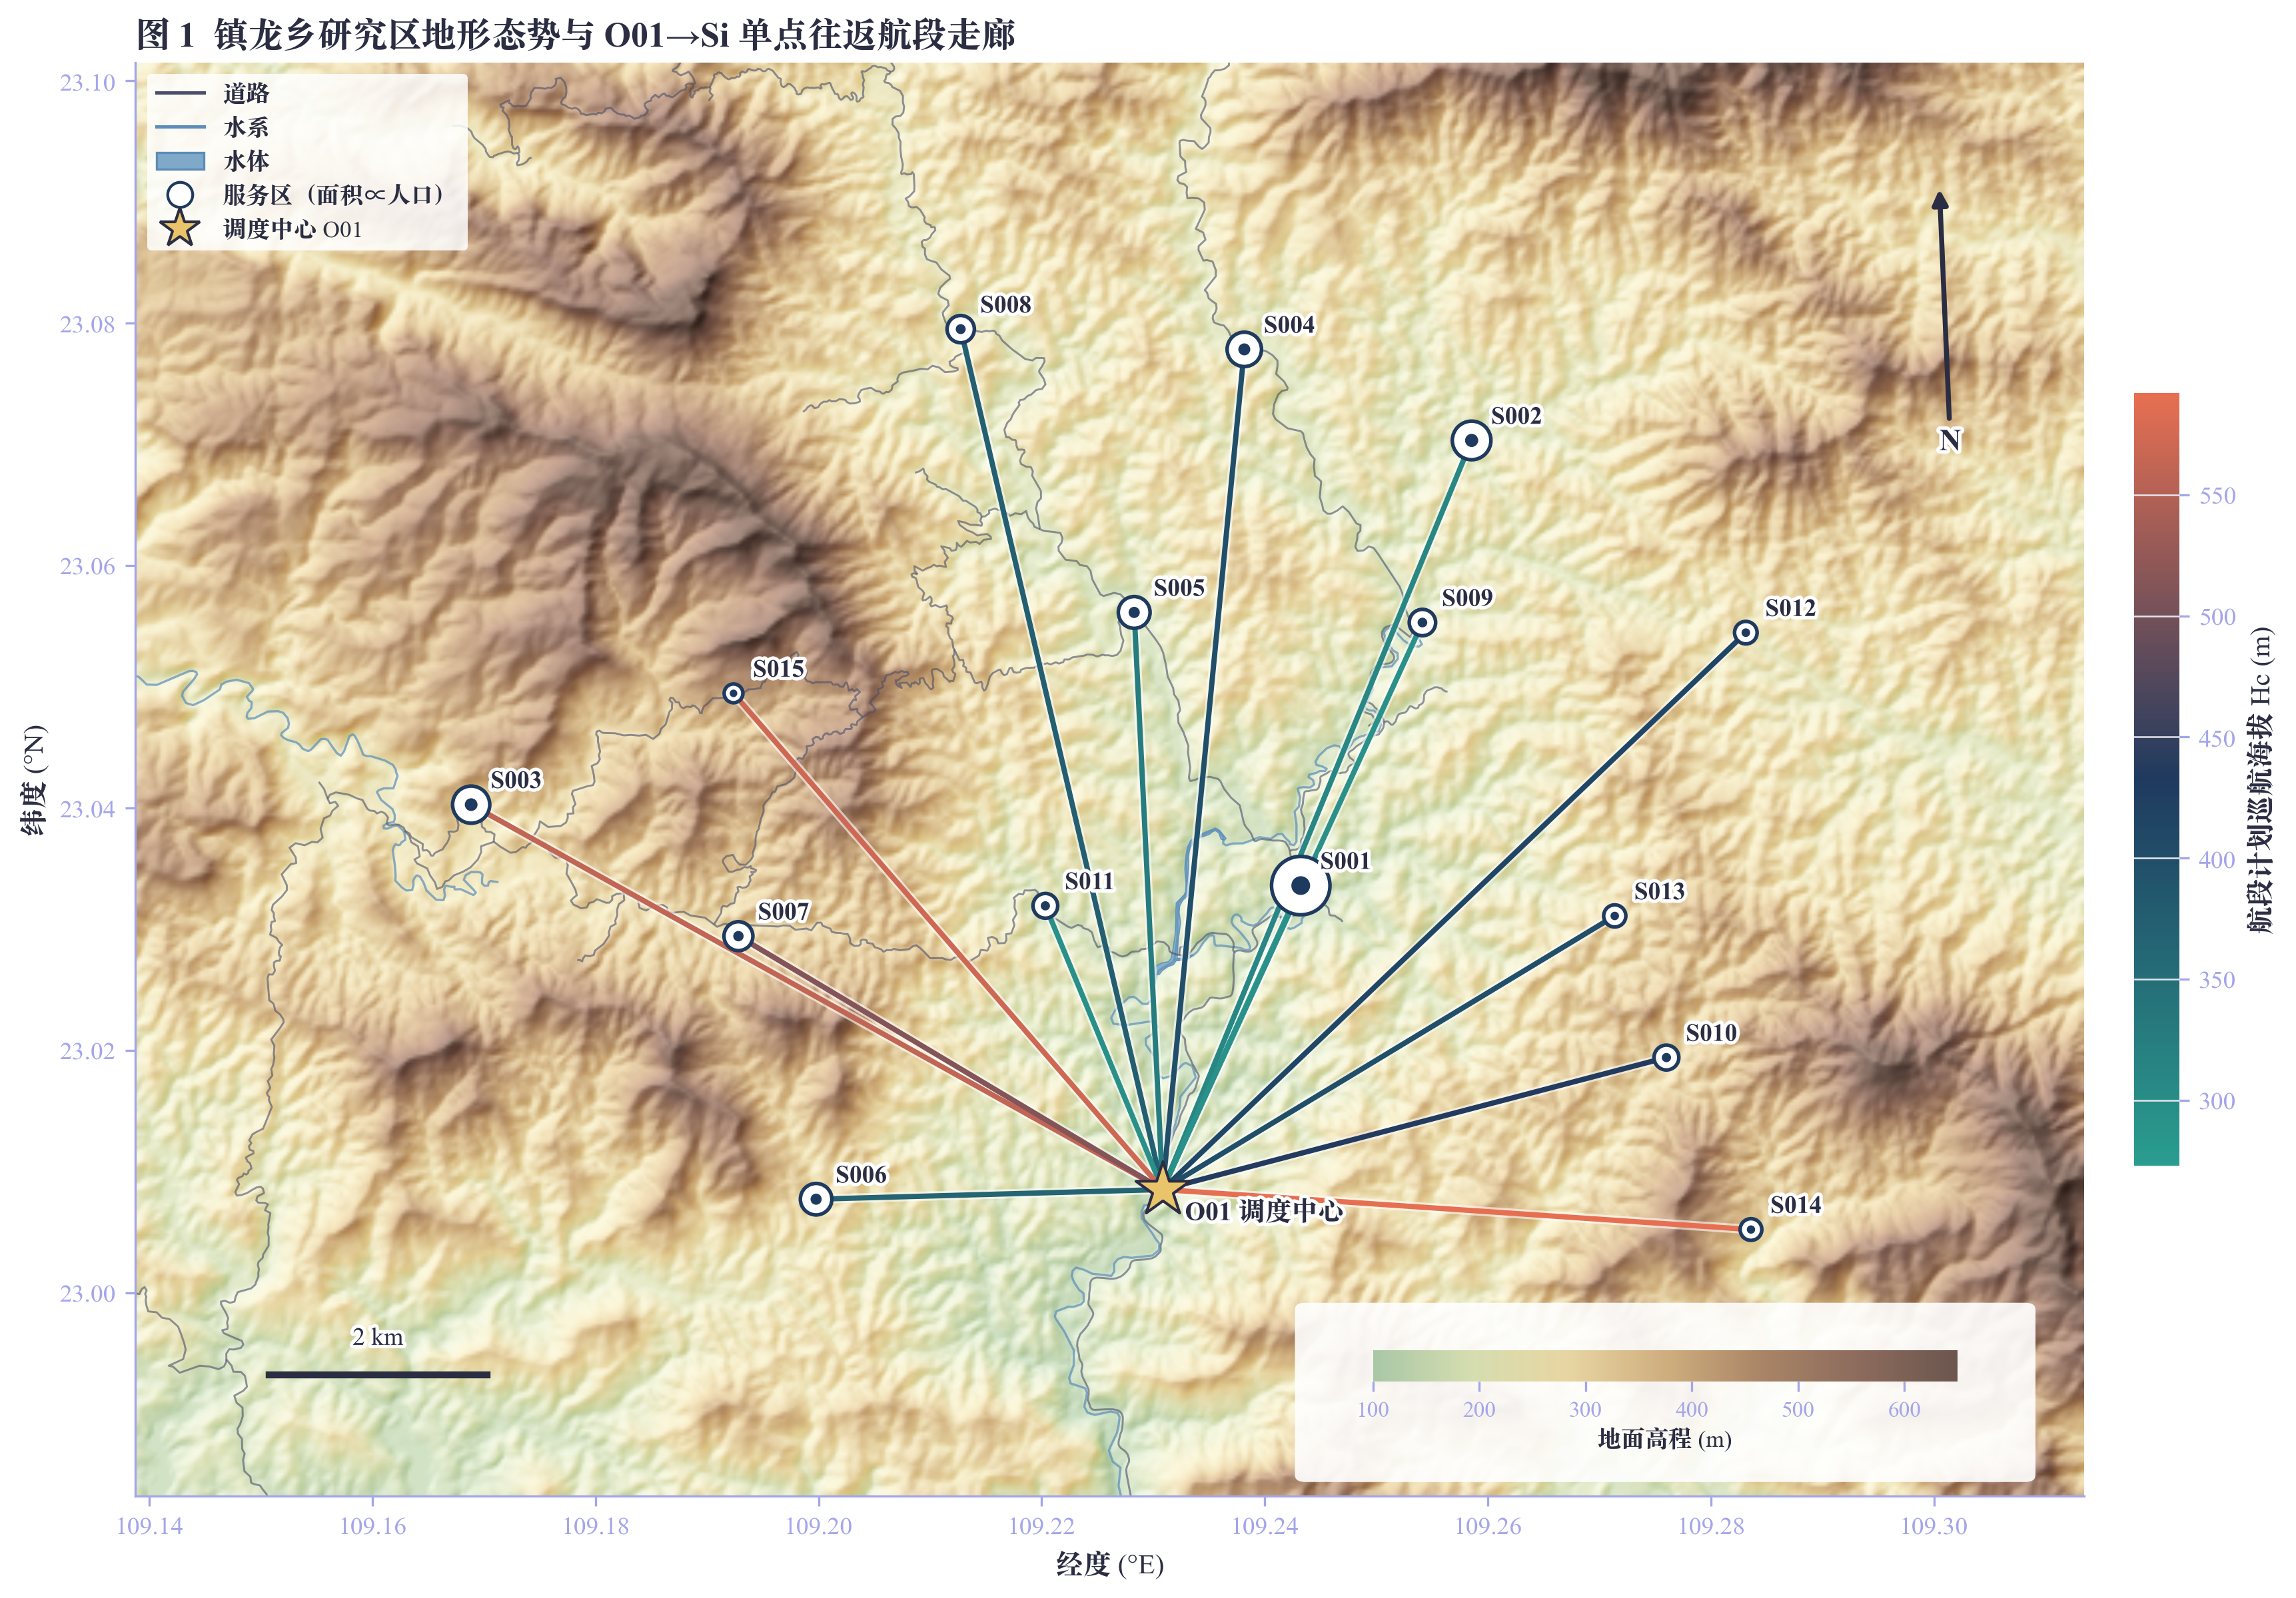
\includegraphics[width=\linewidth]{figures/Q1/图01_研究区地形态势与航段走廊.png}
    \caption{研究区高程栅格与 O01 至 15 个服务区的直线航段}
    \label{fig:q1-route-map}
\end{figure}

\begin{table}[!htbp]
\centering
\caption{O01 至各服务区的航段几何}
\label{tab:route-geometry}
\scriptsize
\setlength{\tabcolsep}{2.5pt}
\renewcommand{\arraystretch}{1.15}
\begin{tabularx}{\textwidth}{
  >{\centering\arraybackslash}p{0.065\textwidth}
  >{\centering\arraybackslash}X
  >{\centering\arraybackslash}p{0.08\textwidth}
  >{\centering\arraybackslash}p{0.07\textwidth}
  >{\centering\arraybackslash}p{0.105\textwidth}
  >{\centering\arraybackslash}p{0.09\textwidth}
  >{\centering\arraybackslash}p{0.10\textwidth}
  >{\centering\arraybackslash}p{0.10\textwidth}
  >{\centering\arraybackslash}p{0.09\textwidth}
}
\toprule
服务区 & 名称
& \shortstack{水平距离\\(km)}
& \shortstack{对应像元\\数}
& \shortstack{沿线最高地面\\(m)}
& \shortstack{巡航海拔\\(m)}
& \shortstack{去程爬升\\(m)}
& \shortstack{去程下降\\(m)}
& \shortstack{服务区海拔\\(m)} \\
\midrule
S001 & 平旺、那龙、镇龙乡 & 3.05 & 136 & 223.06 & 273.06 & 145.36 & 89.06 & 154.00 \\
S002 & 上良 & 7.41 & 323 & 258.95 & 308.95 & 181.25 & 89.45 & 189.50 \\
S003 & 六造、那旭、都长 & 7.26 & 338 & 511.80 & 561.80 & 434.10 & 223.30 & 308.50 \\
S004 & 大站 & 7.71 & 276 & 348.24 & 398.24 & 270.54 & 169.94 & 198.30 \\
S005 & 上良、古律、那麓 & 5.28 & 181 & 276.41 & 326.41 & 198.71 & 131.41 & 165.00 \\
S006 & 六昌、木路 & 3.19 & 116 & 316.10 & 366.10 & 238.40 & 51.30 & 284.80 \\
S007 & 佛子、那桑、银坑 & 4.53 & 213 & 461.97 & 511.97 & 384.27 & 163.47 & 318.50 \\
S008 & 古麻、大站 & 8.08 & 321 & 322.91 & 372.91 & 245.21 & 102.01 & 240.90 \\
S009 & 那龙 & 5.71 & 253 & 243.23 & 293.23 & 165.53 & 63.23 & 200.00 \\
S010 & 镇龙乡 & 4.78 & 203 & 385.64 & 435.64 & 307.94 & 84.04 & 321.60 \\
S011 & 那从 & 2.81 & 123 & 245.36 & 295.36 & 167.66 & 83.26 & 182.10 \\
S012 & 镇龙乡 & 7.39 & 354 & 363.30 & 413.30 & 285.60 & 133.50 & 249.80 \\
S013 & 镇龙乡 & 4.85 & 228 & 349.18 & 399.18 & 271.48 & 47.48 & 321.70 \\
S014 & 镇龙乡 & 5.42 & 203 & 541.95 & 591.95 & 464.25 & 240.95 & 321.00 \\
S015 & 六造、那托、那旭 & 6.01 & 286 & 521.80 & 571.80 & 444.10 & 97.30 & 444.50 \\
\bottomrule
\end{tabularx}
\end{table}

\begin{figure}[H]
\centering
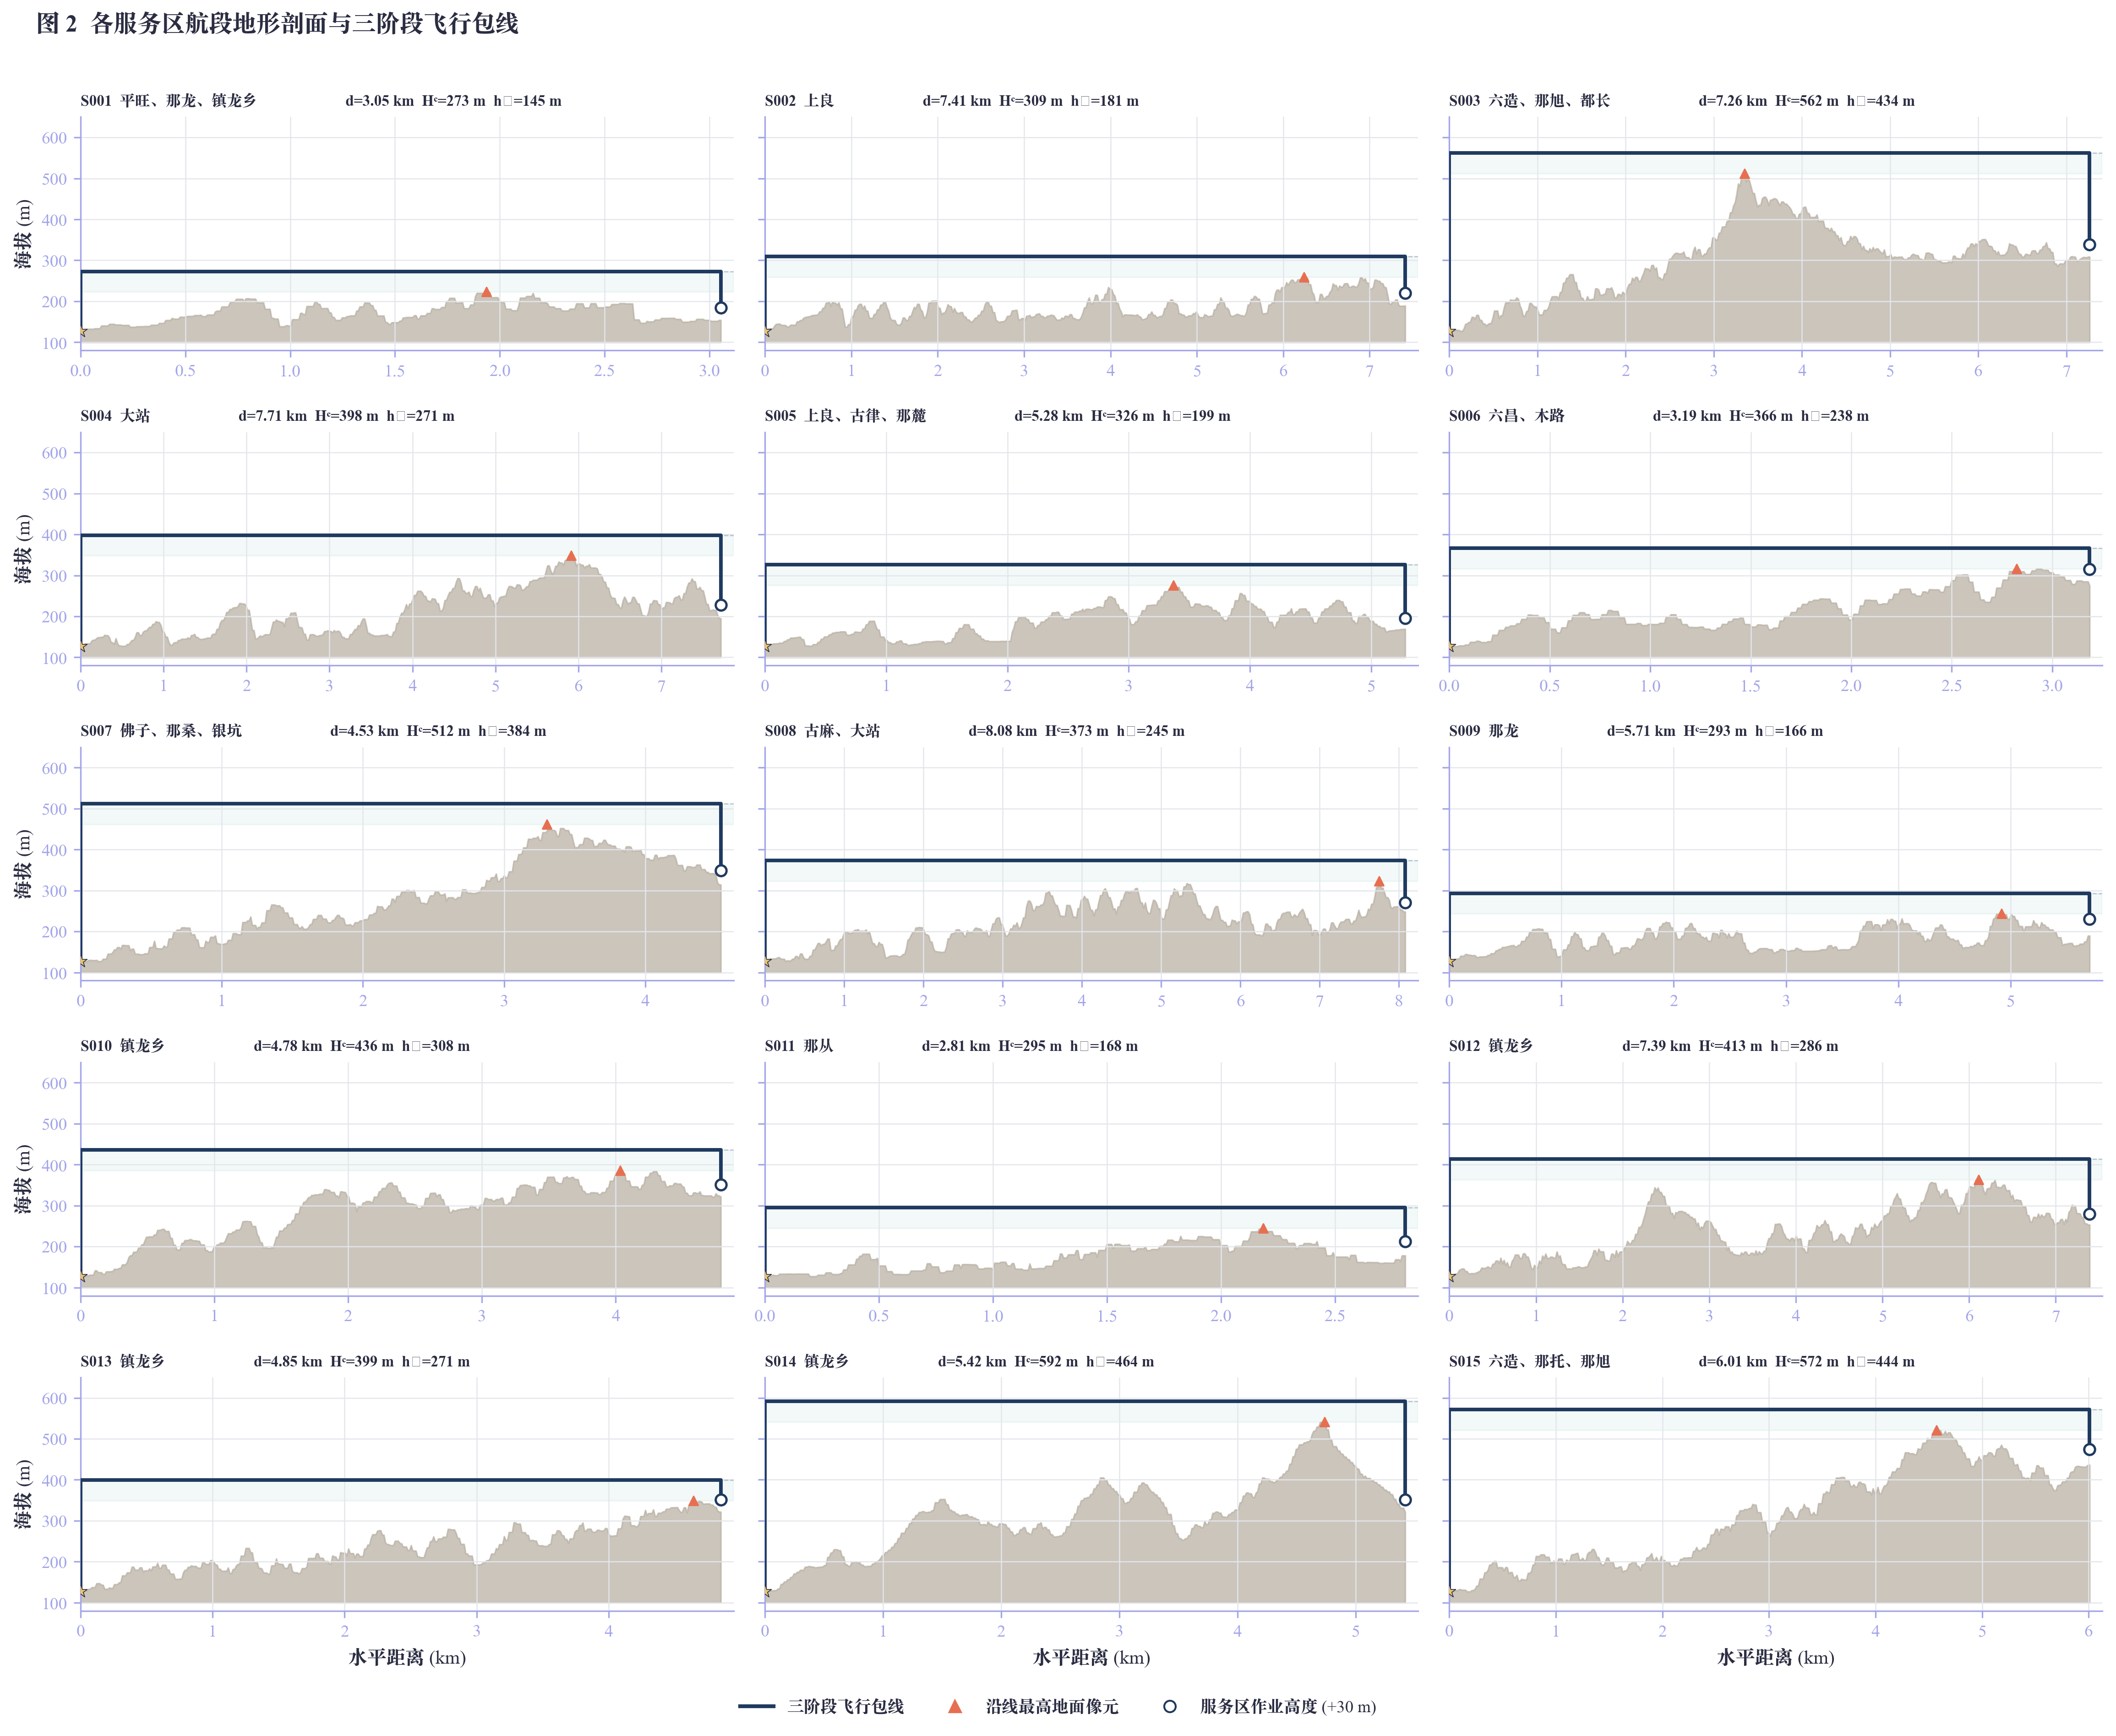
\includegraphics[width=\linewidth]{figures/Q1/图02_航段地形剖面与飞行包线.png}
\caption{15 个服务区航段地形剖面与三阶段飞行包线}
\label{fig:q1-route-profile}
\end{figure}

\begin{figure}[H]
\centering
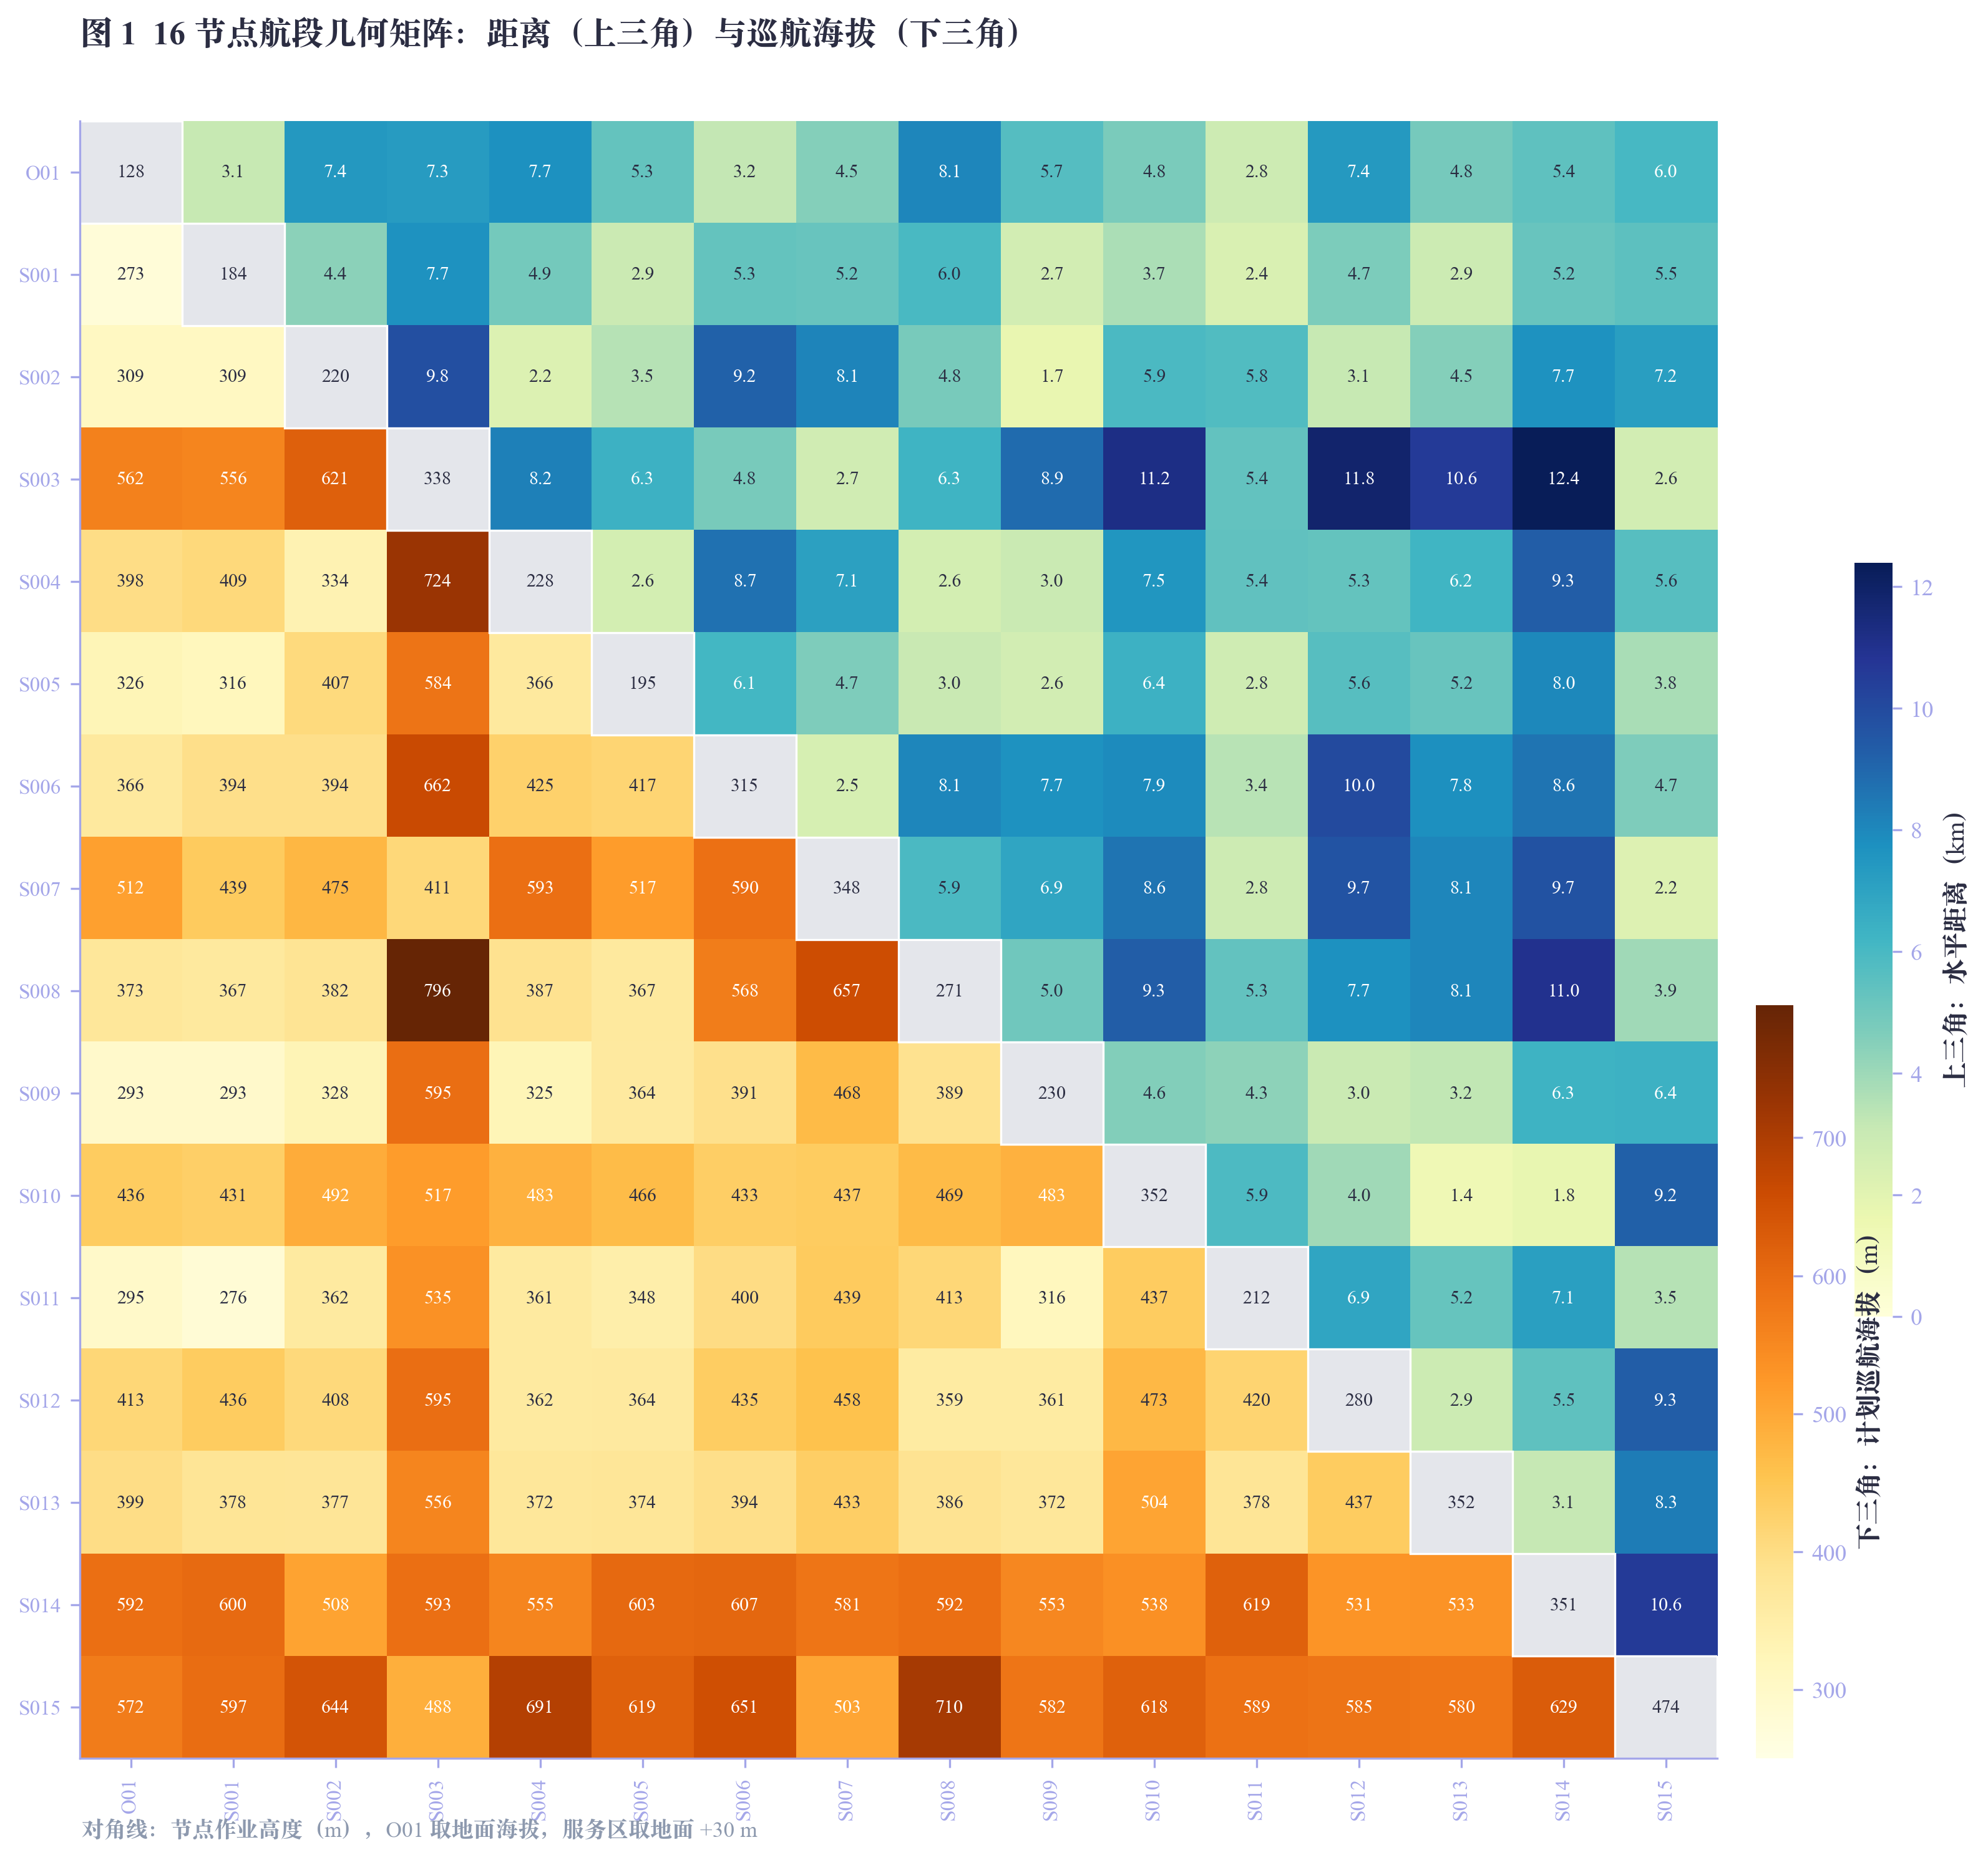
\includegraphics[width=\linewidth]{figures/Q2/图01_航段几何矩阵.png}
\caption{问题二节点间航段距离与巡航海拔矩阵}
\label{fig:q2-geometry}
\end{figure}

\subsection{需求与配送时限结构}

表~\ref{tab:q1-deadlines}汇总期望送达时刻、货箱数及首批截止时刻分布。80 箱中有 30 箱属于首批保障货箱。问题一只用首批标记安排箱号，不把时间窗作为组批约束；问题二则将医疗物资的期望送达时刻和首批货箱的截止时刻作为硬时限，对重合货箱按一个货箱计共 31 箱。其余货箱的期望送达时刻进入及时性指标，并由应急优先系数加权。图~\ref{fig:q2-demand}按服务区展示逐箱需求及两类时限的分布。

\begin{table}[!htbp]
\centering
\caption{逐箱需求的期望送达时刻分布}
\label{tab:q1-deadlines}
\small
\begin{tabular}{@{}cccr@{}}
\toprule
期望送达时刻 & 货箱数 & 总质量（kg） & 首批截止时刻落在该档的货箱数 \\
\midrule
1\,h（3600\,s） & 28 & 315 & 16 \\
2\,h（7200\,s） & 26 & 232 & 7 \\
3\,h（10800\,s） & 18 & 155 & 7 \\
4\,h（14400\,s） & 7 & 50 & 0 \\
5\,h（18000\,s） & 1 & 6 & 0 \\
\midrule
合计 & 80 & 758 & 30 \\
\bottomrule
\end{tabular}
\end{table}

\begin{figure}[H]
\centering
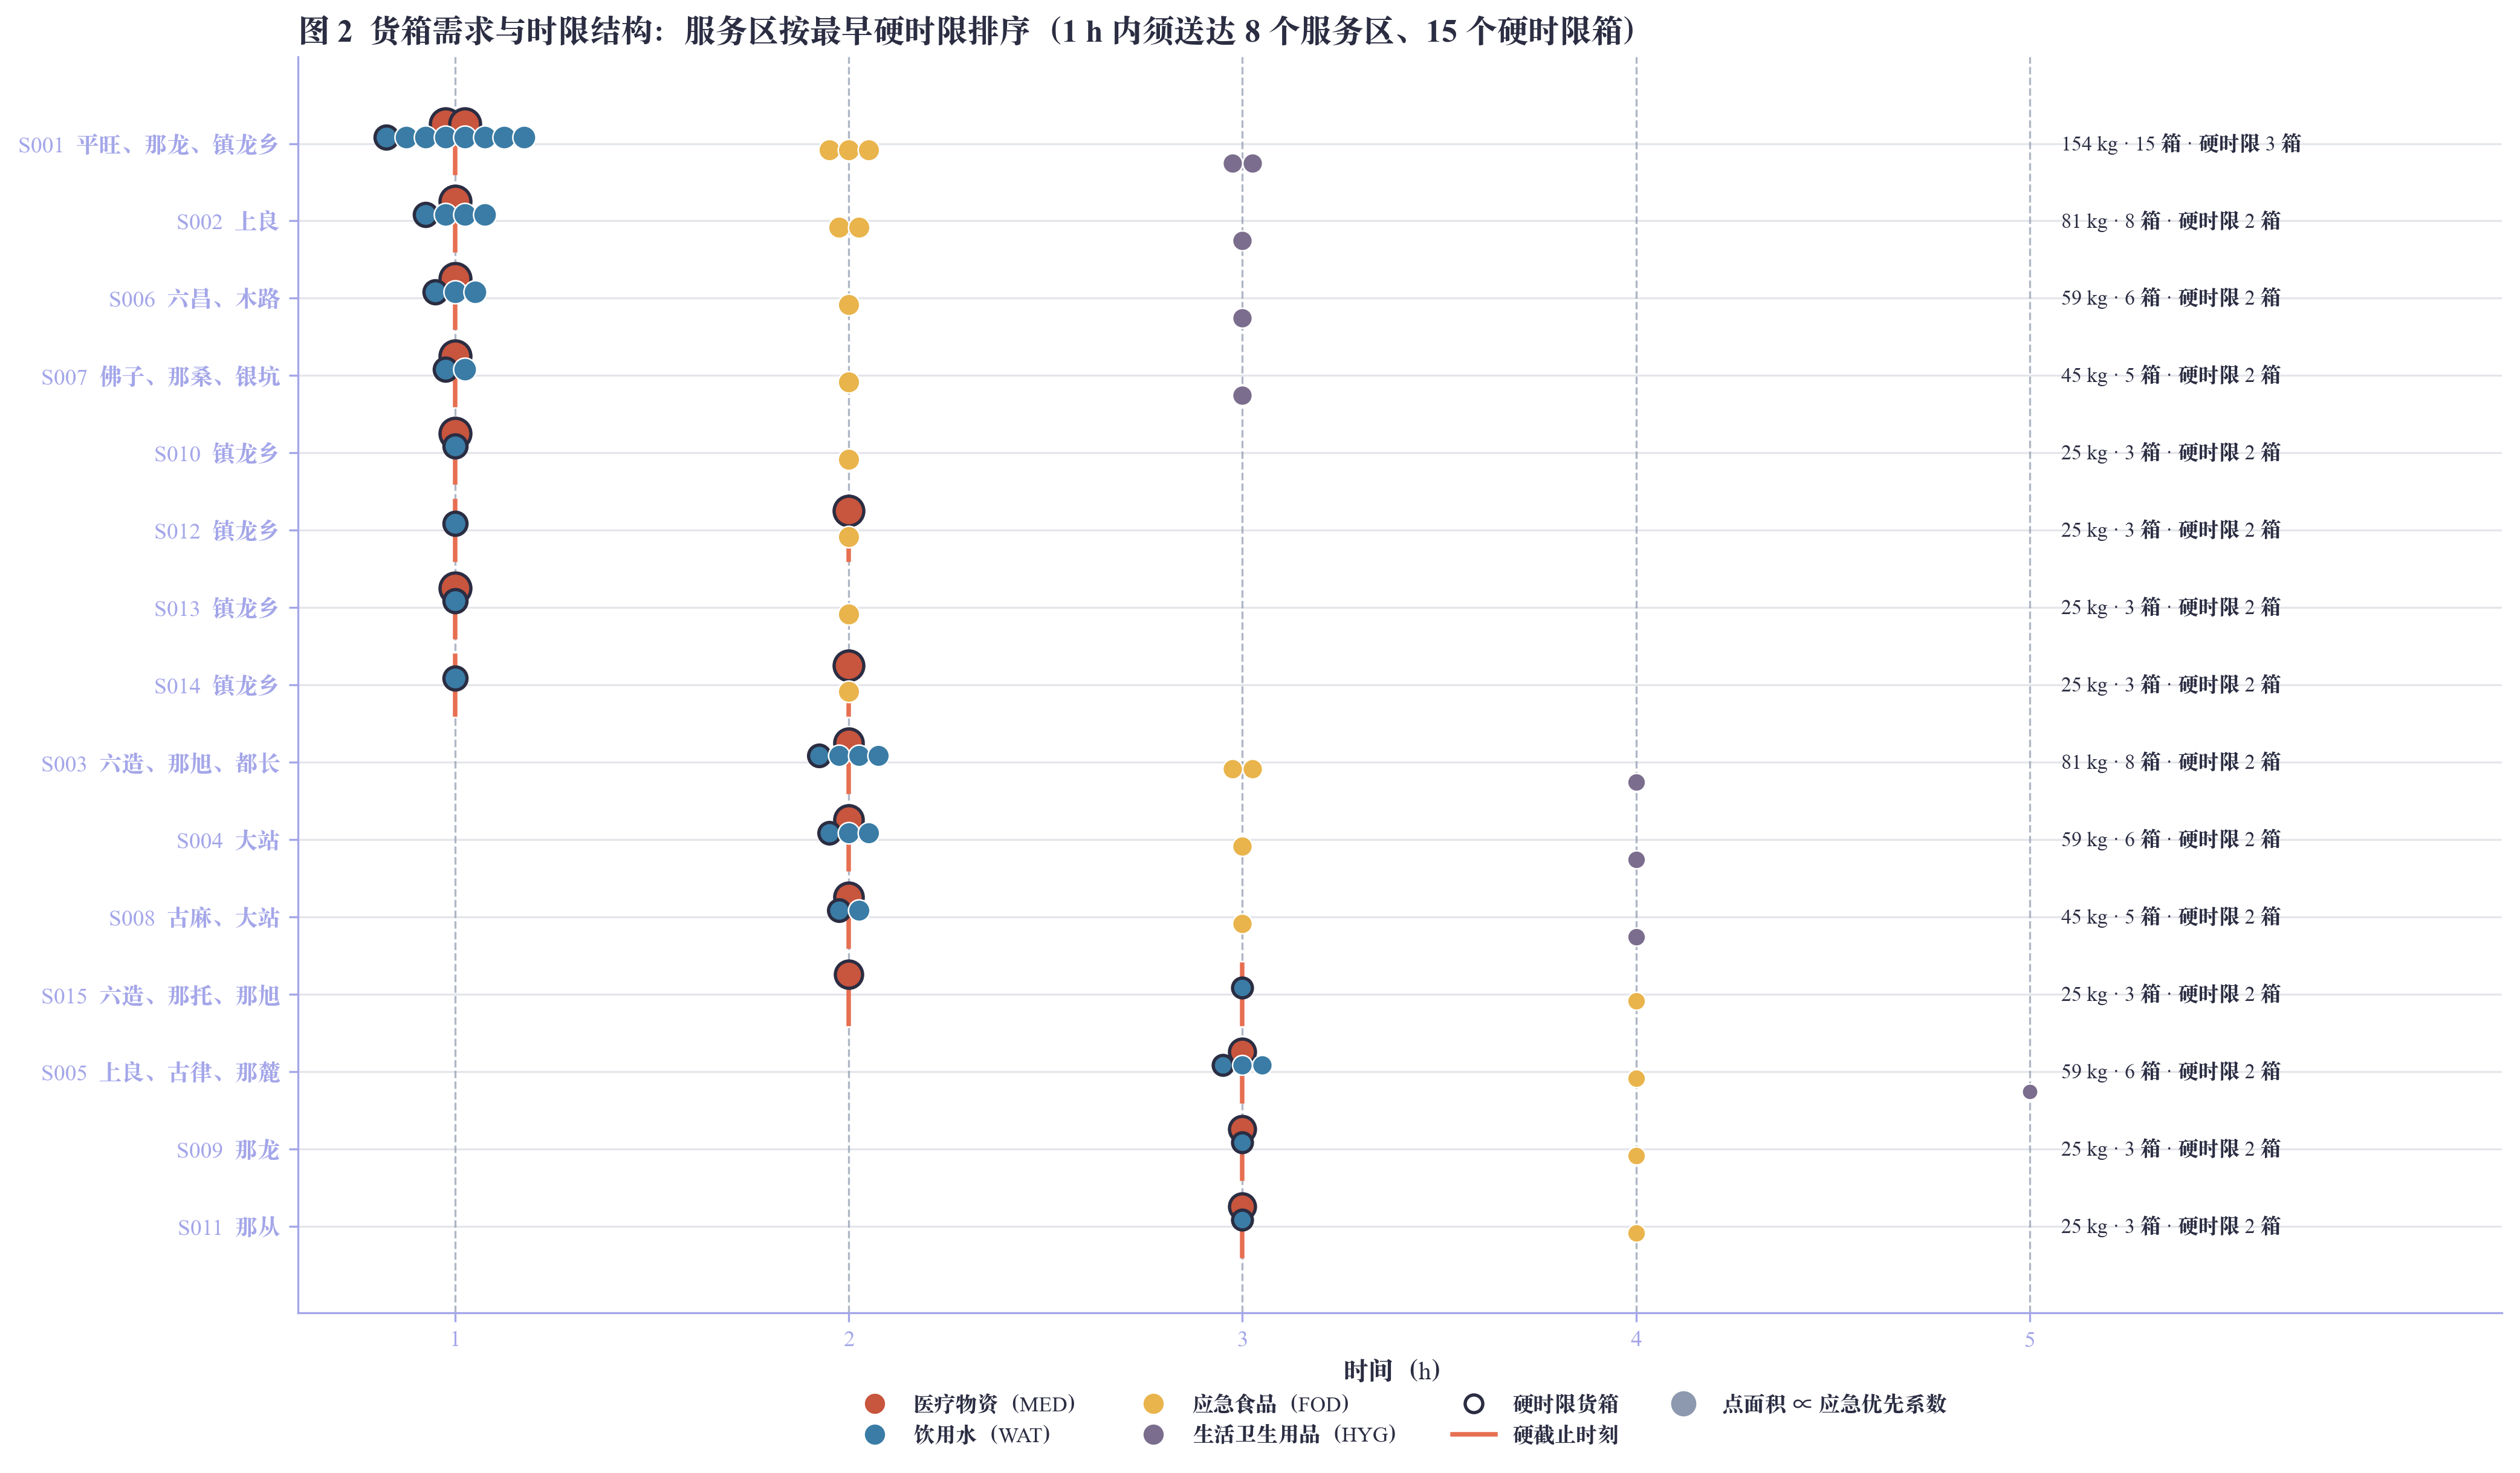
\includegraphics[width=\linewidth]{figures/Q2/图02_需求时限结构图.png}
\caption{服务区逐箱需求、期望送达时刻与首批截止结构}
\label{fig:q2-demand}
\end{figure}

问题二的实体资源为 A 型 4 架、B 型 2 架、C 型 2 架运输无人机，并配有 6、4、4 组对应机型电池；电池从完全放电到充满的等效时间分别为 $1800$、$2400$、$3000\,\mathrm{s}$。表~\ref{tab:q2-resources}列出资源库存，供第七章调度模型使用。

\begin{table}[!htbp]
\centering
\caption{问题二的实体无人机与共享电池库存}
\label{tab:q2-resources}
\small
\begin{tabular}{@{}cccc@{}}
\toprule
机型 & 无人机数量（架） & 电池数量（组） & 完全充电时间（s） \\
\midrule
A & 4 & 6 & 1800 \\
B & 2 & 4 & 2400 \\
C & 2 & 4 & 3000 \\
\bottomrule
\end{tabular}
\end{table}

% 第6章
\vspace{\baselineskip}
\section{问题一：单点往返运输能力与货箱组批模型}

\subsection{问题分析}

问题一要求计算三类机型在 15 个服务区的最大安全载荷，并在货箱不可拆分、不跨服务区组批的条件下，完成全部 80 箱的分批方案。模型分别满足质量、体积和返航能量约束，并比较架次数、总能耗与累计作业时间。实体无人机数量、电池周转和硬时限在问题二中处理。

\subsection{三阶段飞行时间与能耗模型}

设机型为 $g$，服务区为 $i$，单程距离为 $d_i$，去程载荷为 $q$，空载含电池质量为 $m_g^0$。题目给定的载荷—航程关系为
\begin{equation}
L_g(q)=L_g^0-(L_g^0-L_g^F)\left(\frac{q}{Q_g}\right)^{3/2},
\qquad 0\le q\le Q_g .
\label{eq:q1-equivalent-range}
\end{equation}
沿线巡航高度和四段爬升、下降高度由式~\eqref{eq:cruise-altitude}及表~\ref{tab:route-geometry}给出。水平巡航能耗按等效航程折算，爬升能耗按重力势能及爬升效率计算；下降能耗效率为零，因此不另计下降附加能耗。单点往返架次的总能耗为
\begin{equation}
E_{gi}(q)
=
\frac{d_iE_g^{\mathrm{use}}}{L_g(q)}
+\frac{d_iE_g^{\mathrm{use}}}{L_g(0)}
+\frac{(m_g^0+q)g_0h_{i,\mathrm{out}}^+
      +m_g^0g_0h_{i,\mathrm{ret}}^+}
{\eta_g^\uparrow\,3.6\times10^6},
\qquad g_0=9.81\,\mathrm{m/s^2}.
\label{eq:q1-sortie-energy}
\end{equation}
两项水平能耗分别对应载货去程和空载返程，两项爬升使用各自起飞时的质量。载有 $n$ 箱时，飞行时间和总作业时间为
\begin{align}
t_{gi}^{\mathrm{fly}}
&=\frac{h_{i,\mathrm{out}}^+}{v_g^\uparrow}
+\frac{d_i}{v_g^c}
+\frac{h_{i,\mathrm{out}}^-}{v_g^\downarrow}
+\frac{h_{i,\mathrm{ret}}^+}{v_g^\uparrow}
+\frac{d_i}{v_g^c}
+\frac{h_{i,\mathrm{ret}}^-}{v_g^\downarrow},\\
T_{gi}(n)
&=t_g^{\mathrm{prep}}+nt_g^{\mathrm{load}}
+t_{gi}^{\mathrm{fly}}+t_g^{\mathrm{hand}}+nt_g^{\mathrm{box}} .
\label{eq:q1-sortie-time}
\end{align}
其中 $t_g^{\mathrm{prep}}$、$t_g^{\mathrm{load}}$、$t_g^{\mathrm{hand}}$ 和 $t_g^{\mathrm{box}}$ 分别为固定准备、单箱装载、基础交接和单箱交接时间。本问的累计作业时间为各架次时间之和，不含多机并行及电池周转，因而不等于问题二的完工时间。无人机参数见表~\ref{tab:q1-uav-parameters}。

\begin{table}[!htbp]
\centering
\caption{运输无人机模型的主要参数}
\label{tab:q1-uav-parameters}
\footnotesize
\setlength{\tabcolsep}{3pt}
\renewcommand{\arraystretch}{1.1}
\begin{tabular}{@{}cccccccc@{}}
\toprule
机型
& $m_0$（kg）
& \shortstack{$Q_g$（kg）\\$V_g$（m$^3$)}
& $v_g^c$（m/s）
& $L_g^0/L_g^F$（m）
& $E_g^{\mathrm{use}}/\rho$（kWh/\%）
& \shortstack{$v_g^\uparrow/v_g^\downarrow$\\$\eta_g^\uparrow$}
& \shortstack{$t_g^{\mathrm{prep}}/t_g^{\mathrm{load}}$\\$t_g^{\mathrm{hand}}/t_g^{\mathrm{box}}$（s）} \\
\midrule
A & 70.0 & 25/0.060 & 12 & 25000/20000 & 4.5/20 & 3/2.5/0.72 & 300/30/150/30 \\
B & 65.0 & 30/0.073 & 15 & 28000/16000 & 4.0/20 & 3/2.5/0.72 & 300/30/150/30 \\
C & 69.9 & 80/0.250 & 15 & 26000/12000 & 8.0/20 & 2.5/2/0.72 & 300/30/180/36 \\
\bottomrule
\end{tabular}
\end{table}

图~\ref{fig:q1-energy-budget}预留各机型能耗预算曲线与载荷拆分示意。

\begin{figure}[H]
\centering
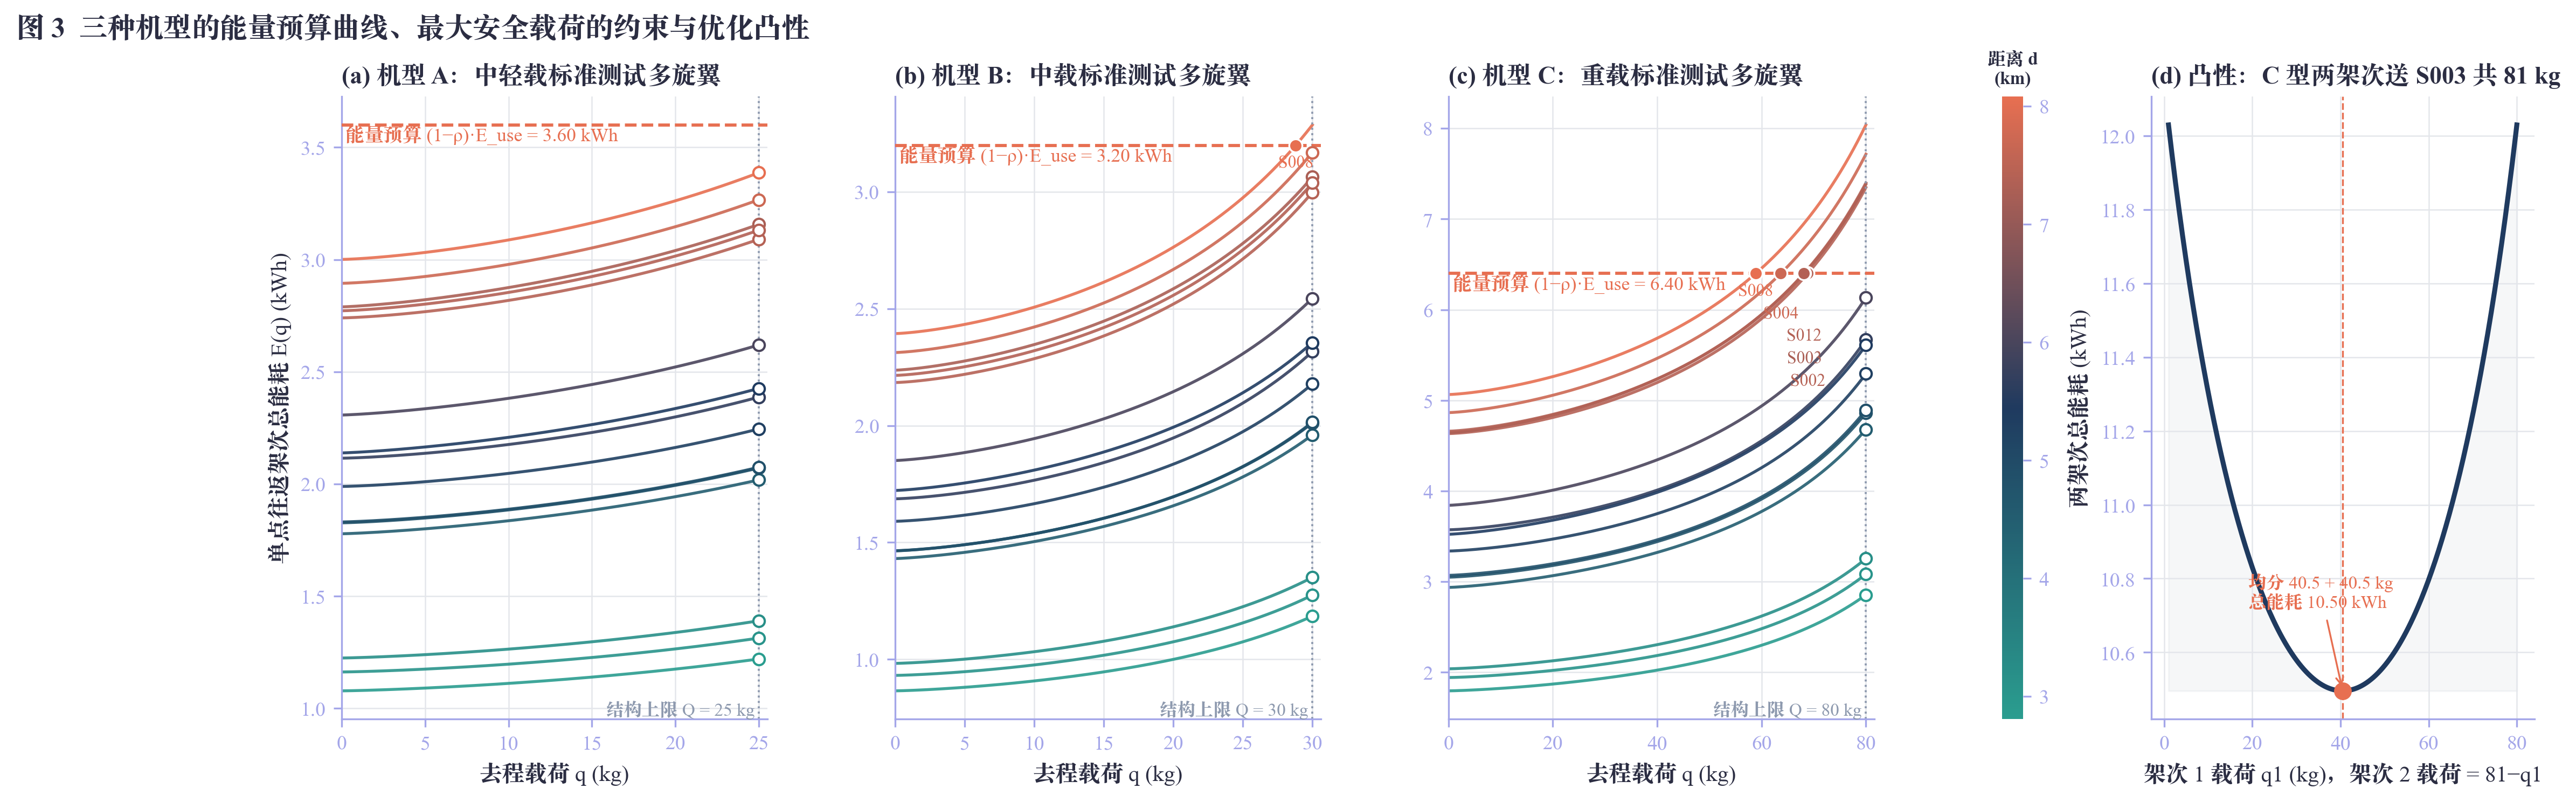
\includegraphics[width=\linewidth]{figures/Q1/图03_能量预算曲线.png}
\caption{三种机型的往返能耗预算曲线与 S003 两架次载荷拆分}
\label{fig:q1-energy-budget}
\end{figure}

\subsection{最大安全载荷}

对机型 $g$ 和服务区 $i$，最大安全载荷为满足返航余量的最大去程载荷：
\begin{equation}
q_{gi}^{\max}
=
\max\left\{q\in[0,Q_g]:
E_{gi}(q)\le(1-\rho_g)E_g^{\mathrm{use}}\right\}.
\label{eq:q1-qmax}
\end{equation}
$E_{gi}(q)$ 随 $q$ 单调递增：若结构满载可行，则 $q_{gi}^{\max}=Q_g$；若空载往返超出预算，则该组合不可行；其余情形用 60 次二分搜索求根。基准返航余量为 $\rho_g=0.20$，结果见表~\ref{tab:q1-qmax}。

\begin{table}[!htbp]
\centering
\caption{基准返航安全余量下各服务区的最大安全载荷（kg）}
\label{tab:q1-qmax}
\small
\begin{tabular}{@{}cccc@{}}
\toprule
服务区 & 机型 A & 机型 B & 机型 C \\
\midrule
S001 & 25.00 & 30.00 & 80.00 \\
S002 & 25.00 & 30.00 & 68.86 \\
S003 & 25.00 & 30.00 & 68.21 \\
S004 & 25.00 & 30.00 & 63.70 \\
S005 & 25.00 & 30.00 & 80.00 \\
S006 & 25.00 & 30.00 & 80.00 \\
S007 & 25.00 & 30.00 & 80.00 \\
S008 & 25.00 & 28.80 & 58.90 \\
S009 & 25.00 & 30.00 & 80.00 \\
S010 & 25.00 & 30.00 & 80.00 \\
S011 & 25.00 & 30.00 & 80.00 \\
S012 & 25.00 & 30.00 & 68.12 \\
S013 & 25.00 & 30.00 & 80.00 \\
S014 & 25.00 & 30.00 & 80.00 \\
S015 & 25.00 & 30.00 & 80.00 \\
\bottomrule
\end{tabular}
\end{table}

机型 A 在 15 个服务区均受 $25\,\mathrm{kg}$ 结构上限约束；机型 B 仅在 S008 受能量约束；机型 C 在 S002、S003、S004、S008 和 S012 的能量约束先于 $80\,\mathrm{kg}$ 结构上限生效。图~\ref{fig:q1-payload}预留最大安全载荷与距离的对照。

\begin{figure}[H]
\centering
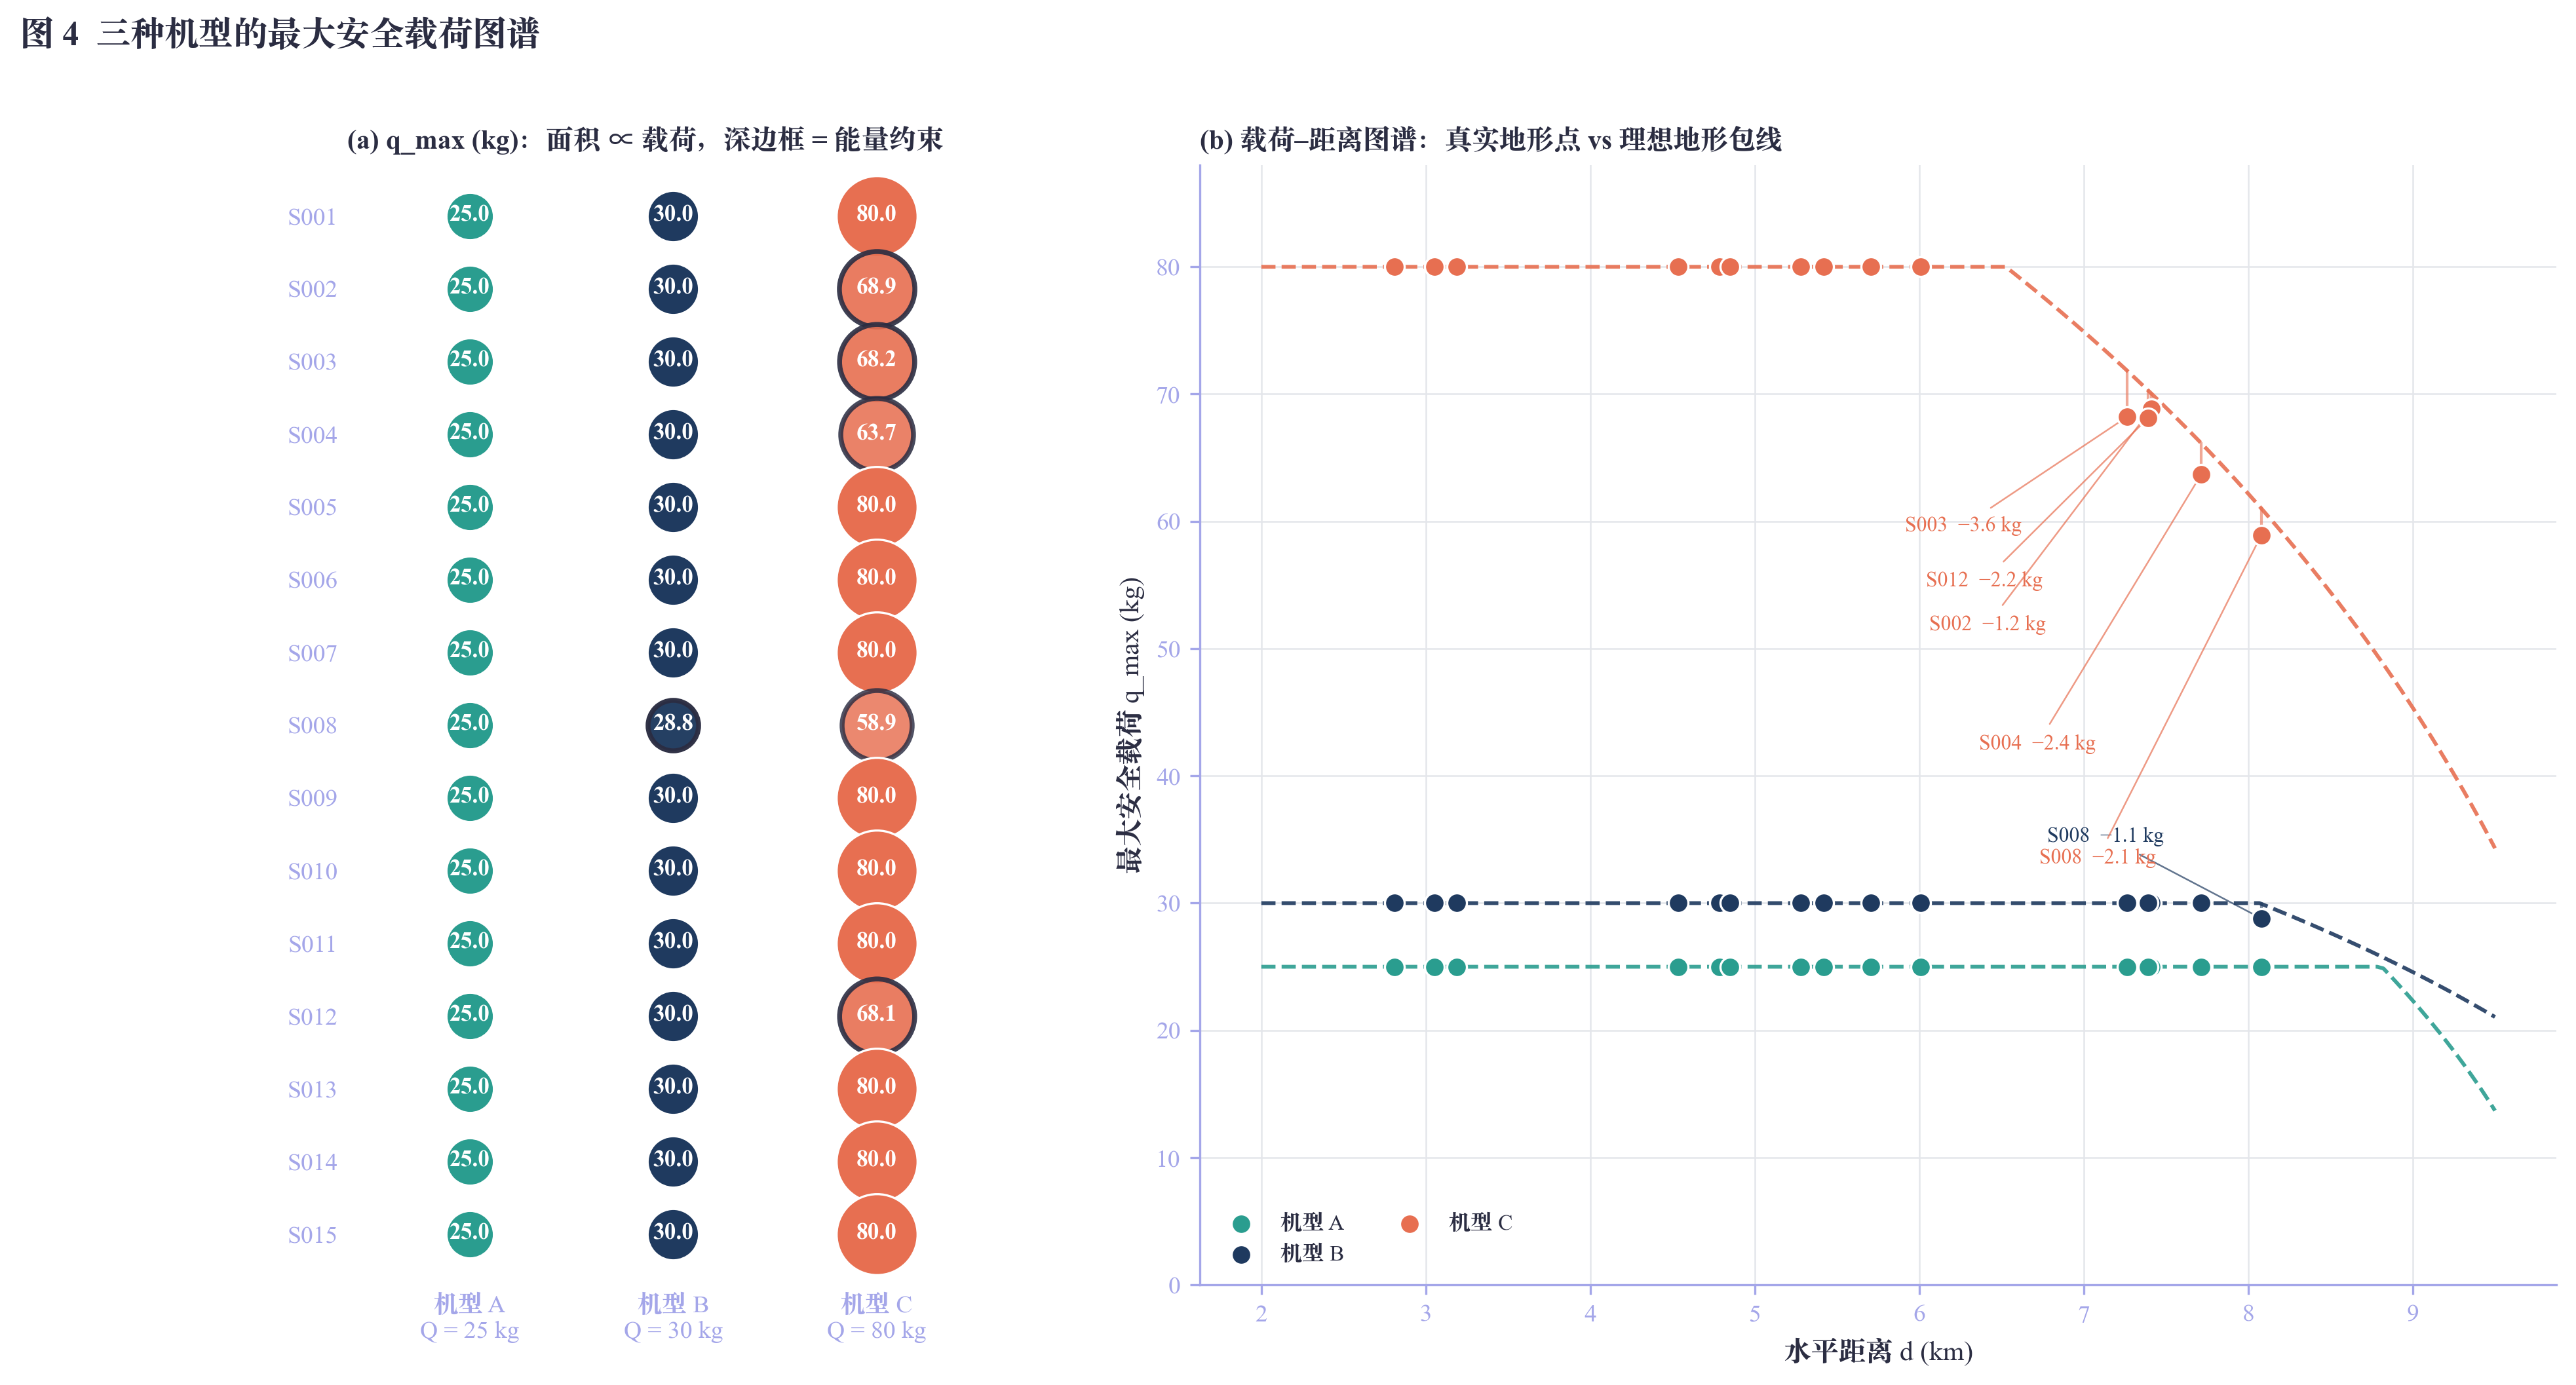
\includegraphics[width=\linewidth]{figures/Q1/图04_最大安全载荷图谱.png}
\caption{各服务区最大安全载荷随水平距离的变化及结构上限}
\label{fig:q1-payload}
\end{figure}

\subsection{货箱组批的精确多目标动态规划}

同一服务区内同类货箱的质量、体积相同，因此一个架次可用四类货箱的箱数向量 $\boldsymbol n=(n_k)_{k=1}^4$ 表示。设服务区 $i$ 的剩余需求为 $\boldsymbol r_i$，装载模式 $p=(g,\boldsymbol n_p)$ 可行当且仅当
\[
\boldsymbol 0\ne\boldsymbol n_p\le\boldsymbol r_i,\qquad
\sum_k n_{pk}m_k\le q_{gi}^{\max},\qquad
\sum_k n_{pk}v_k\le V_g .
\]
对应的三指标代价为
\[
\boldsymbol c_p=
\left(1,\ E_{gi}\!\left(\sum_k n_{pk}m_k\right),\
T_{gi}\!\left(\sum_k n_{pk}\right)\right).
\]
在剩余需求状态上递推并保留非支配解：
\begin{equation}
\mathcal F_i(\boldsymbol r)
=
\operatorname{Pareto}\left\{
\boldsymbol c_p+\boldsymbol f:
\boldsymbol n_p\le\boldsymbol r,\quad
\boldsymbol f\in\mathcal F_i(\boldsymbol r-\boldsymbol n_p)
\right\},
\quad
\mathcal F_i(\boldsymbol 0)=\{(0,0,0)\}.
\label{eq:q1-pareto-dp}
\end{equation}
若解的架次、能耗和时间均不优于另一解且至少一项严格较差，则将其删除。每个服务区的需求状态有限，模式代价可加，故动态规划给出该离散模式集合下的精确 Pareto 前沿；服务区之间无资源耦合，全局前沿由各区前沿逐项相加后再筛除支配解得到。

\subsection{组批结果与三指标权衡}

在全局前沿上比较四种决策规则：R1 按架次、能耗、时间作字典序优先；R2 按能耗、架次、时间优先；R3 按累计时间、架次、能耗优先；R4 将各指标除以其理想值后等权求和。结果见表~\ref{tab:q1-rules}。全局精确前沿有两个方案：架次优先方案为 18 架次、$59.131\,\mathrm{kWh}$、$9.104\,\mathrm{h}$；能耗优先方案为 19 架次、$59.034\,\mathrm{kWh}$、$9.567\,\mathrm{h}$。因此节省 $0.097\,\mathrm{kWh}$ 的代价是增加 1 架次和 $0.463\,\mathrm{h}$ 累计作业时间。

\begin{table}[!htbp]
\centering
\caption{不同决策规则选出的全局组批方案}
\label{tab:q1-rules}
\small
\begin{tabular}{@{}lccccc@{}}
\toprule
规则 & 优先顺序 & 架次 $N$ & 能耗 $E$（kWh） & 时间 $T$（h） & 机型（A/B/C） \\
\midrule
R1 架次优先 & $N\to E\to T$ & 18 & 59.131 & 9.104 & 0/9/9 \\
R2 能耗优先 & $E\to N\to T$ & 19 & 59.034 & 9.567 & 0/11/8 \\
R3 时间优先 & $T\to N\to E$ & 18 & 59.131 & 9.104 & 0/9/9 \\
R4 均衡折中 & 理想值归一后等权 & 18 & 59.131 & 9.104 & 0/9/9 \\
\bottomrule
\end{tabular}
\end{table}

R1 方案中 S001、S002、S003 各分为两架次，其余服务区各一架次；80 箱均分配一次，且各架次满足质量、体积和能量约束。表~\ref{tab:q1-fleet-policy}比较不同机型可用集合：加入 C 型机后，架次数由仅 B 型的 35 次降至 18 次，总能耗降至 $59.131\,\mathrm{kWh}$。

\begin{table}[!htbp]
\centering
\caption{不同机型可用集合下的组批指标}
\label{tab:q1-fleet-policy}
\small
\begin{tabular*}{0.90\textwidth}{@{\extracolsep{\fill}}lccc@{}}
\toprule
机型集合 & 架次 $N$ & 能耗 $E$（kWh） & 累计时间 $T$（h） \\
\midrule
仅 A & 52 & 112.180 & 24.813 \\
仅 B & 35 & 68.351 & 15.460 \\
仅 C & 18 & 73.935 & 9.400 \\
A+B & 35 & 68.351 & 15.460 \\
A+B+C（R1） & 18 & 59.131 & 9.104 \\
\bottomrule
\end{tabular*}
\end{table}

图~\ref{fig:q1-batch-plan}预留逐箱组批方案，图~\ref{fig:q1-indicator-tradeoffs}预留机型策略比较。R1 方案去程水平巡航能耗为 $33.94\,\mathrm{kWh}$，返程为 $22.63\,\mathrm{kWh}$，合计约占总能耗的 $95.7\%$；爬升能耗约占 $4.3\%$。

累计作业时间为 $9.104\,\mathrm{h}$，其中飞行约 $5.36\,\mathrm{h}$，地面准备、装载和交接约 $3.75\,\mathrm{h}$。减少架次会同步减少地面作业时间，但累计作业时间不等于并行调度的完工时间。图~\ref{fig:q1-energy-time}预留分区能耗与时间构成。

\begin{figure}[H]
\centering
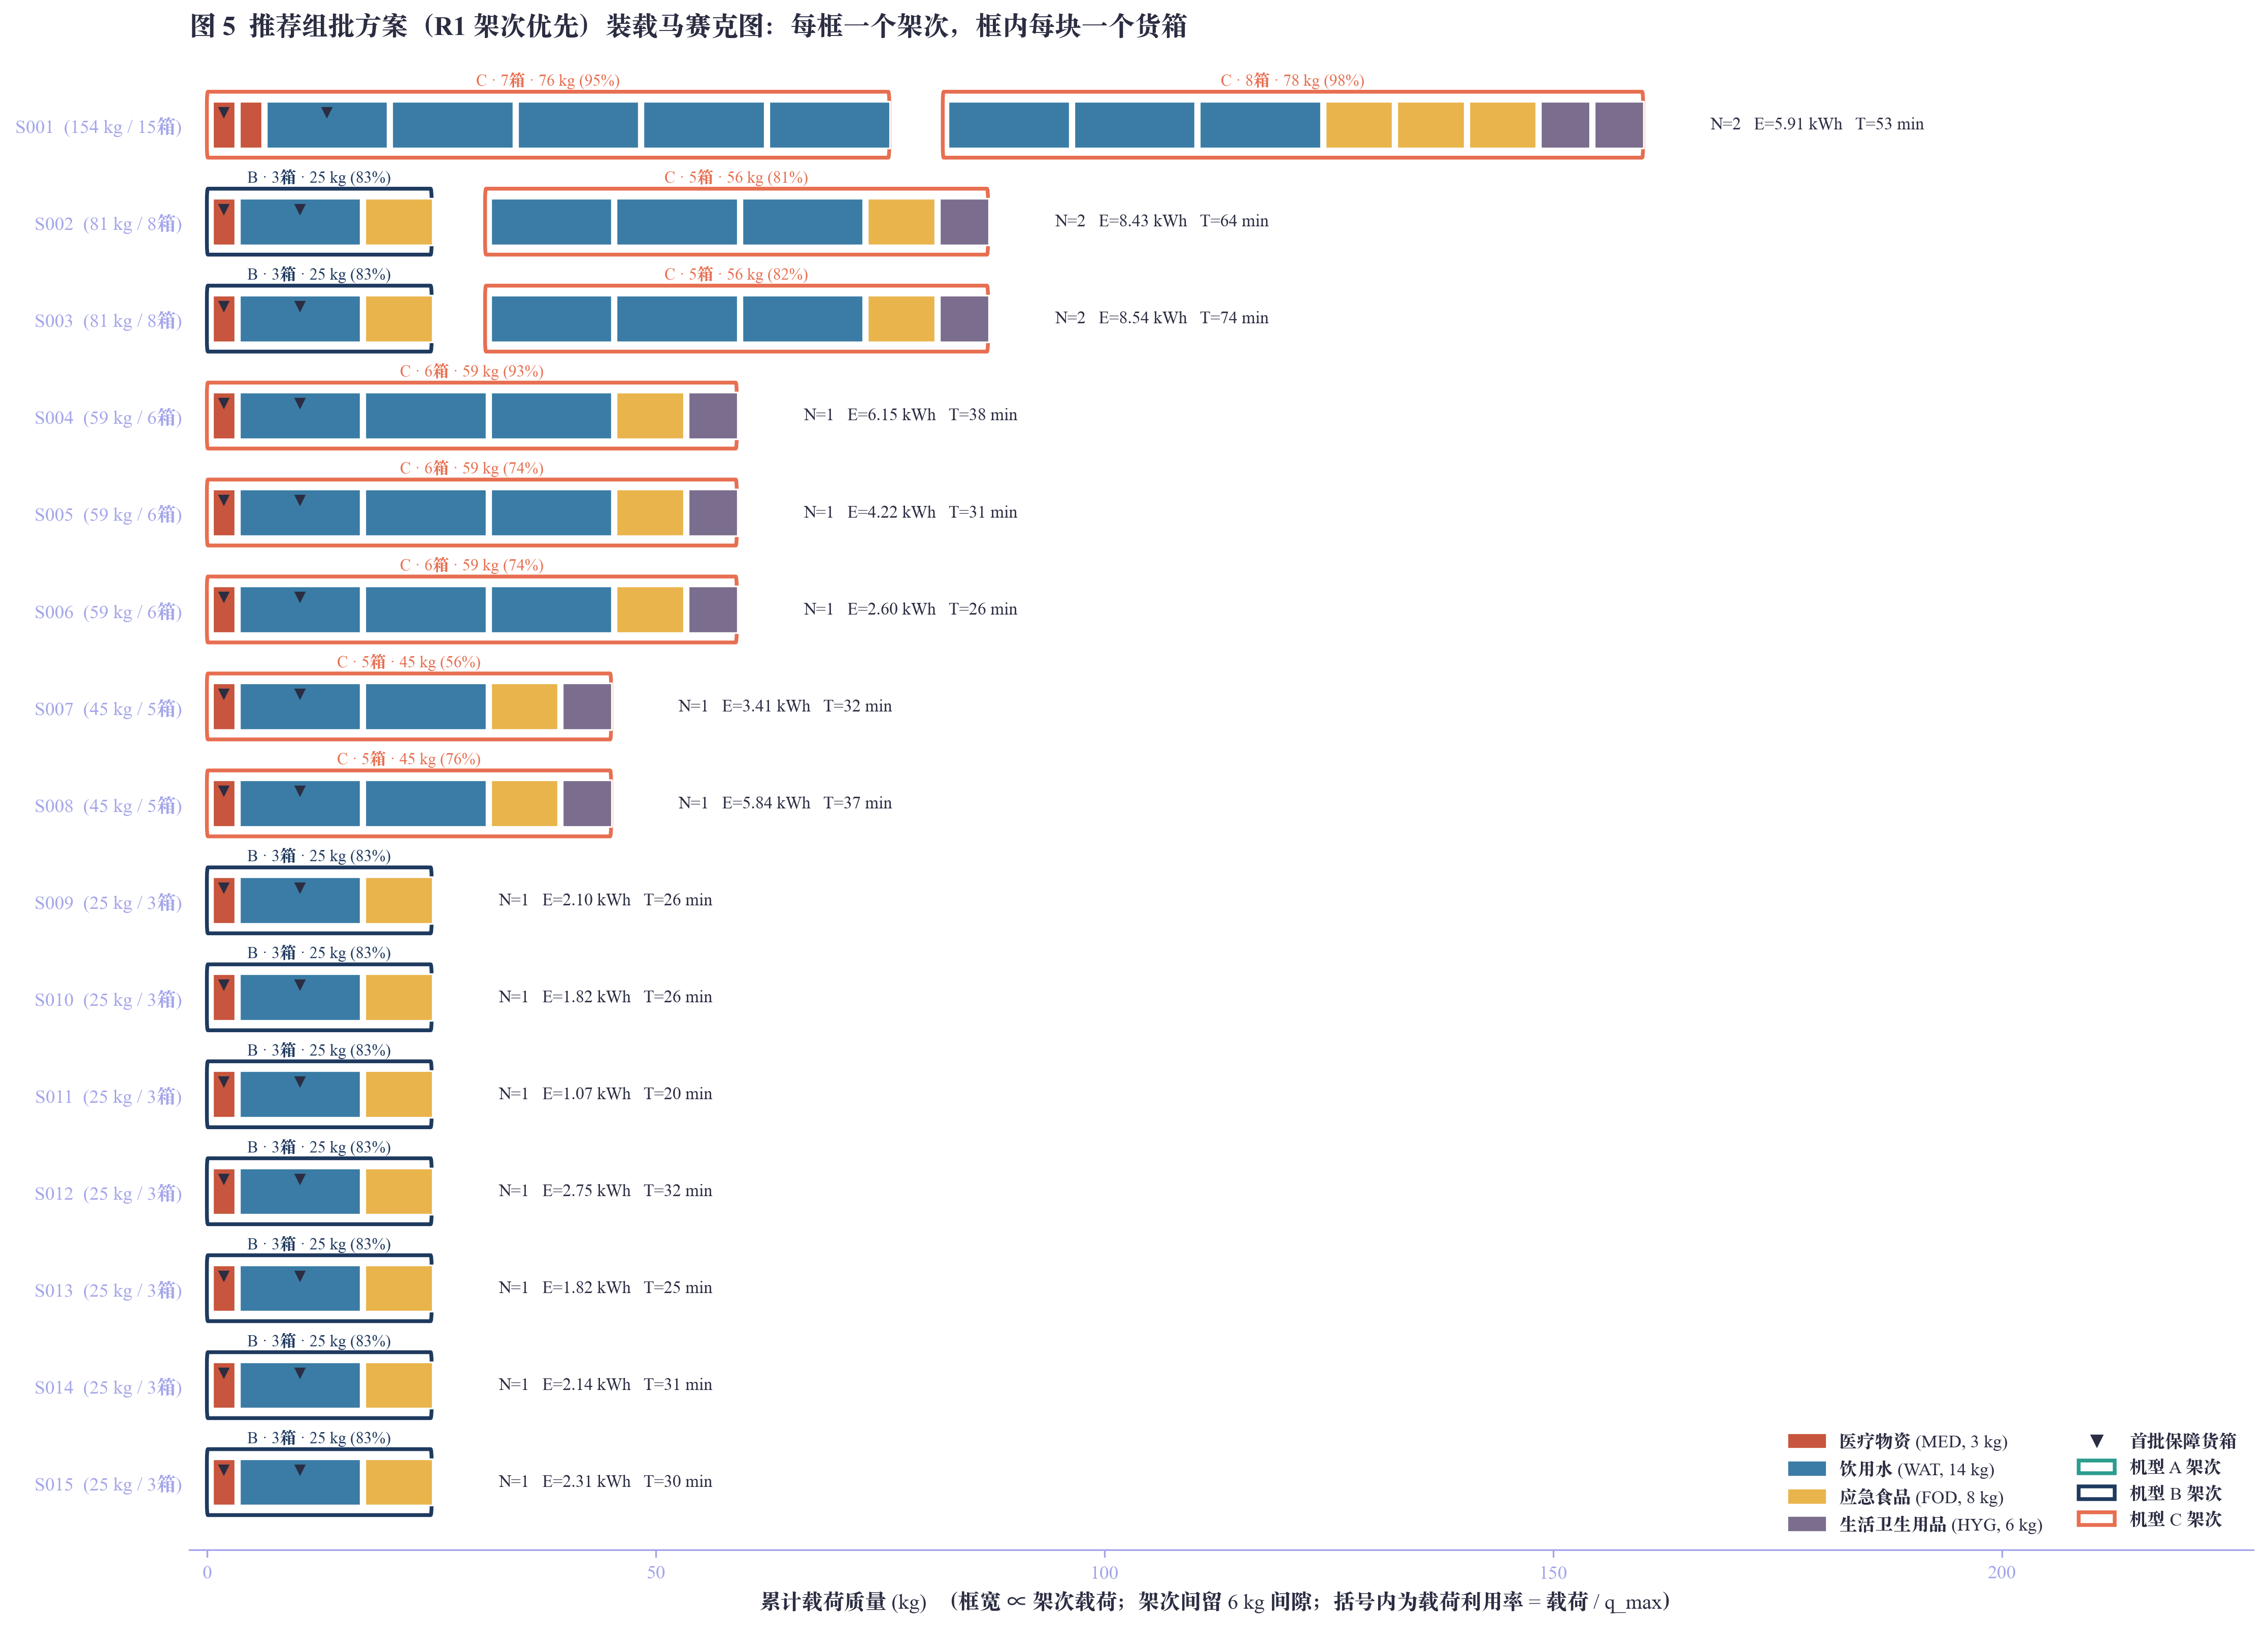
\includegraphics[width=\linewidth]{figures/Q1/图05_组批方案装载马赛克图.png}
\caption{R1 规则下各服务区逐箱组批方案}
\label{fig:q1-batch-plan}
\end{figure}

\begin{figure}[H]
\centering
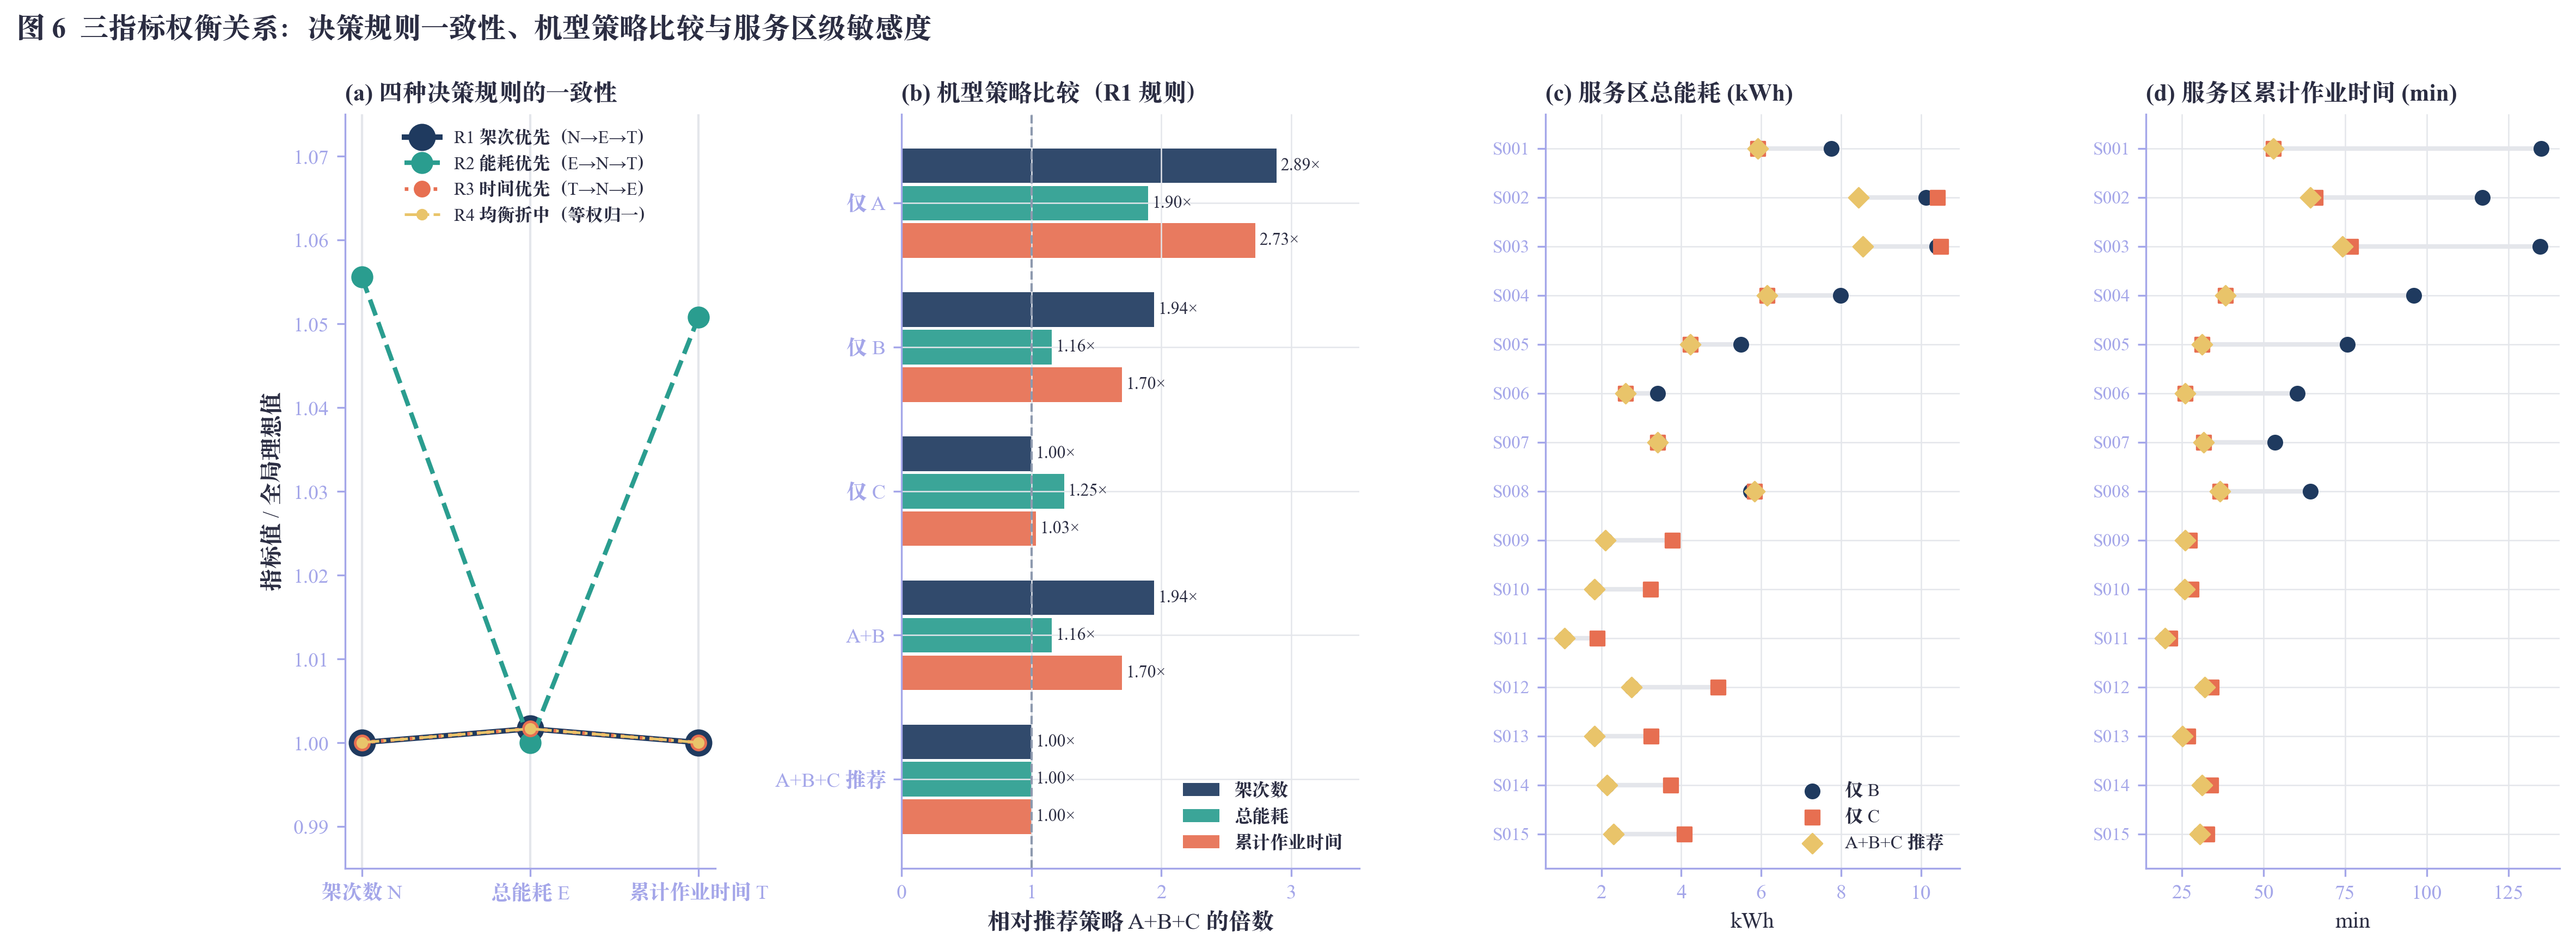
\includegraphics[width=\linewidth]{figures/Q1/图06_指标权衡与机型策略.png}
\caption{三指标权衡、决策规则一致性与机型策略比较}
\label{fig:q1-indicator-tradeoffs}
\end{figure}

\begin{figure}[H]
\centering
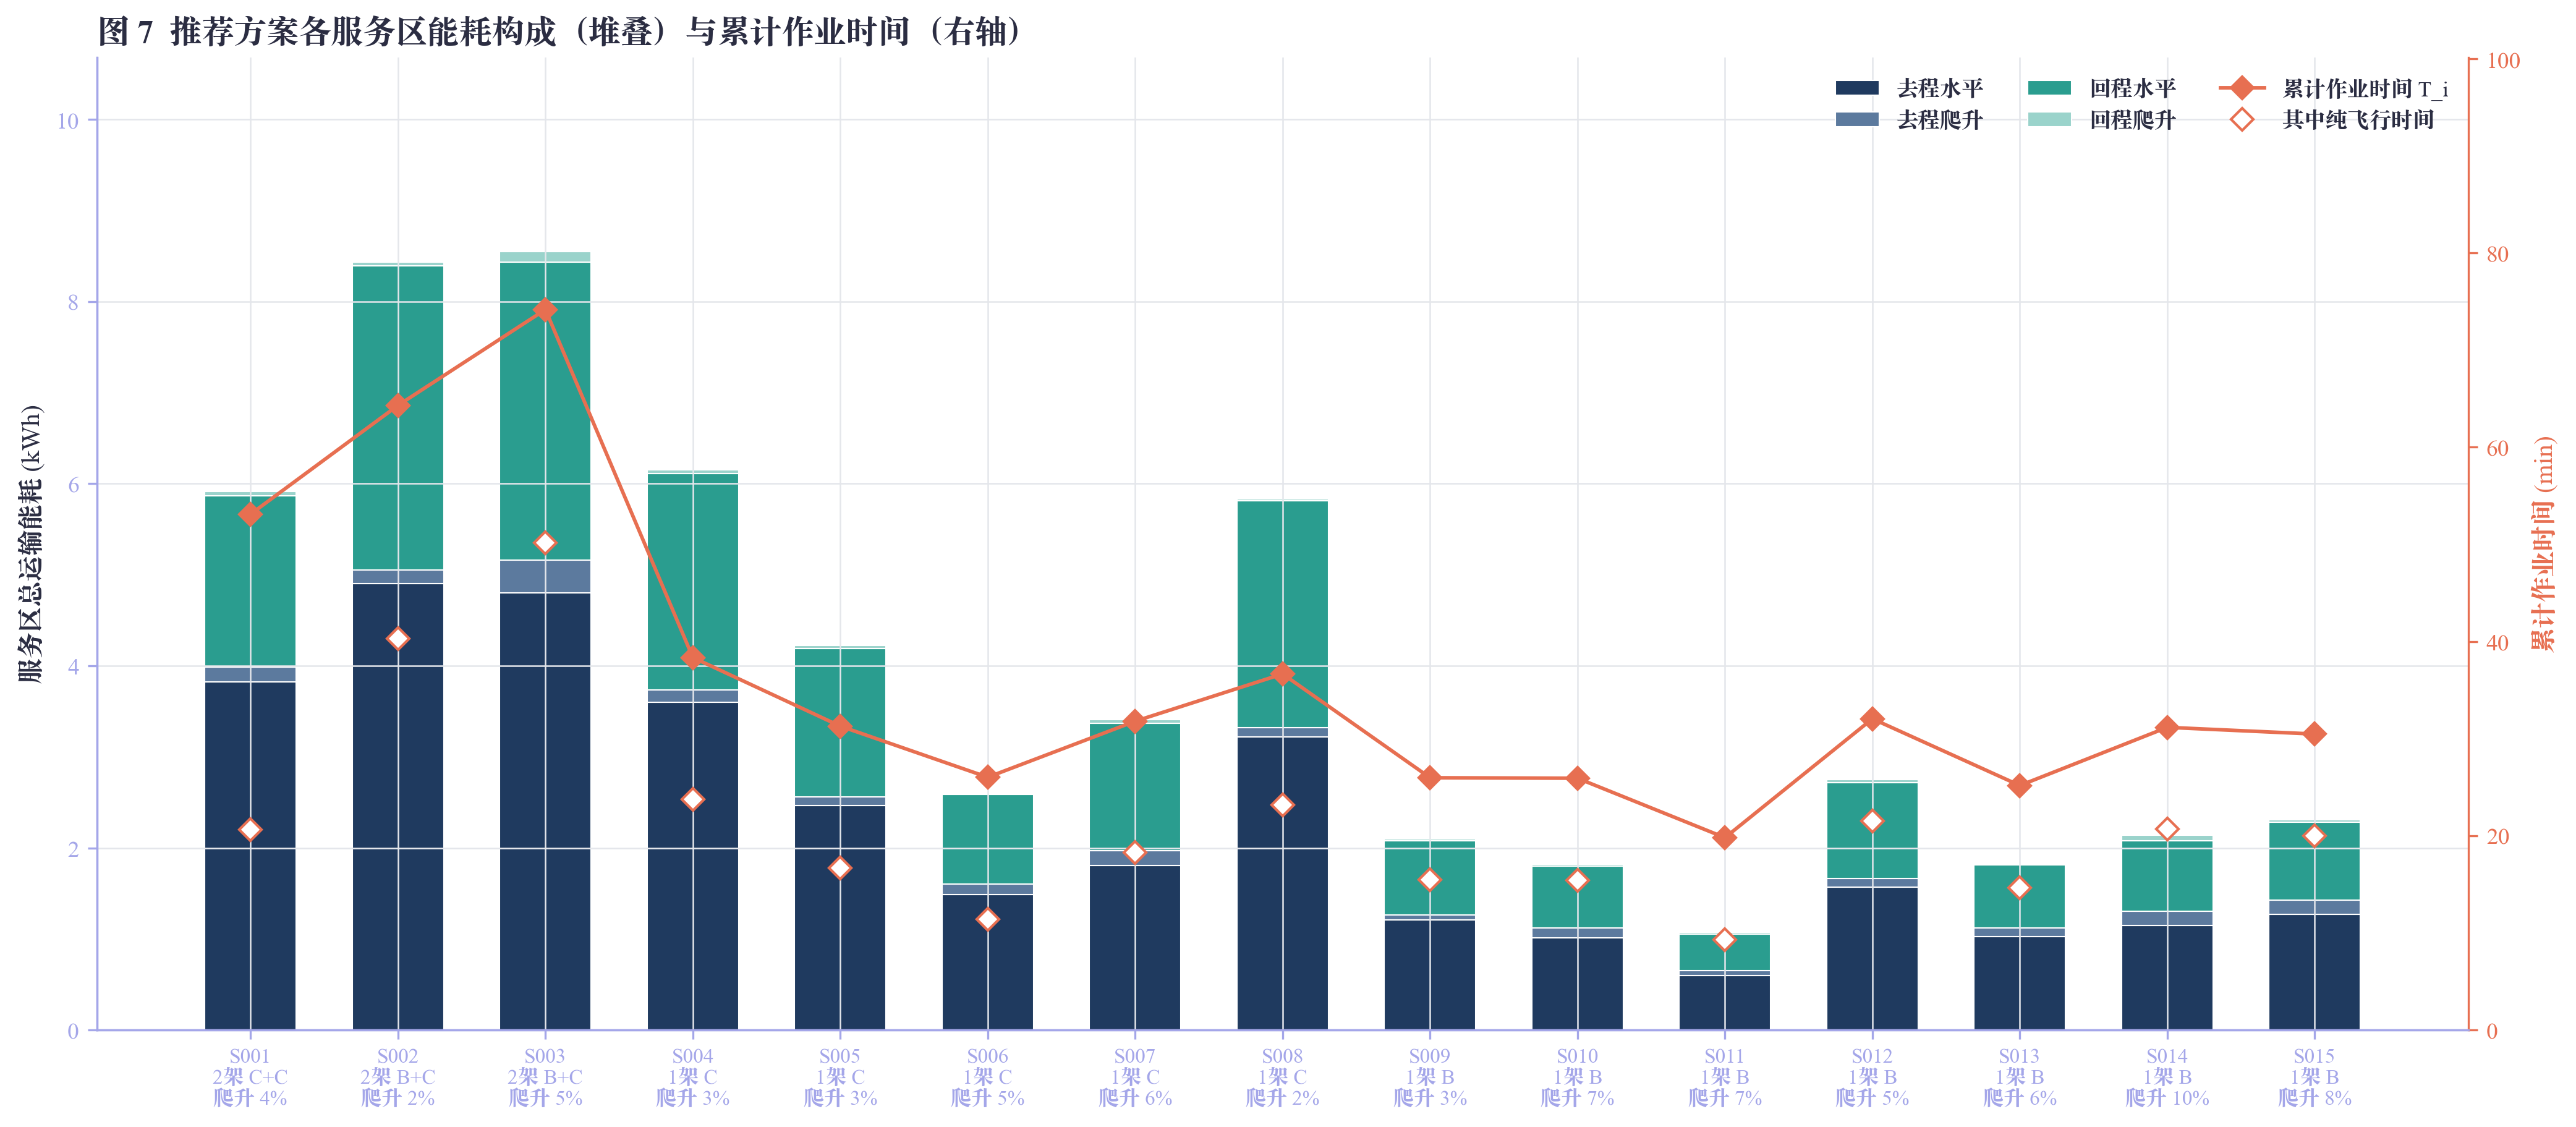
\includegraphics[width=\linewidth]{figures/Q1/图07_能耗构成与作业时间.png}
\caption{推荐组批方案的分区能耗构成与累计作业时间}
\label{fig:q1-energy-time}
\end{figure}

\subsection{返航安全余量的敏感性分析}

将三种机型的返航安全余量统一设为 $\rho\in[0.05,0.45]$，以 $0.01$ 为步长；每个取值下重新计算最大安全载荷并求解组批。表~\ref{tab:q1-rho-summary}列出基准点及代表值。扫描网格中，完整覆盖全部服务区的最大余量为 $0.35$；$\rho=0.36$ 时 S008 首先无法完成全部配送。

\begin{table}[!htbp]
\centering
\caption{返航安全余量变化下的组批结果}
\label{tab:q1-rho-summary}
\small
\begin{tabular}{@{}ccccc@{}}
\toprule
$\rho$ & 完整覆盖 & 架次 $N$ & 能耗 $E$（kWh） & 时间 $T$（h） \\
\midrule
0.20 & 是 & 18 & 59.131 & 9.104 \\
0.25 & 是 & 19 & 61.073 & 9.602 \\
0.30 & 是 & 20 & 67.228 & 10.163 \\
0.35 & 是 & 25 & 75.608 & 12.607 \\
0.36 & 否，S008 未覆盖 & -- & -- & -- \\
\bottomrule
\end{tabular}
\end{table}

定义能量约束开始限制结构载荷的余量阈值及空载往返失效阈值为
\[
\rho_{gi}^{\mathrm{cap}}=1-\frac{E_{gi}(Q_g)}{E_g^{\mathrm{use}}},
\qquad
\rho_{gi}^{\mathrm{inf}}=1-\frac{E_{gi}(0)}{E_g^{\mathrm{use}}}.
\]
当 $\rho\le\rho_{gi}^{\mathrm{cap}}$ 时结构满载可行；当 $\rho_{gi}^{\mathrm{cap}}<\rho\le\rho_{gi}^{\mathrm{inf}}$ 时仅部分载荷可行；当 $\rho>\rho_{gi}^{\mathrm{inf}}$ 时空载往返也不可行。S008 在 $\rho=0.36$ 时，A 型空载已不可行，B、C 型最大安全载荷分别约为 $12.7\,\mathrm{kg}$ 和 $8.6\,\mathrm{kg}$，均低于单箱饮用水质量 $14\,\mathrm{kg}$，因而无法覆盖该区全部需求。该扫描只针对问题一单点往返组批，不含问题二的多机并行、电池周转及配送硬时限。图~\ref{fig:q1-rho-sensitivity}和图~\ref{fig:q1-rho-window}预留载荷、全局指标及分区架次数的敏感性结果。

\begin{figure}[H]
\centering
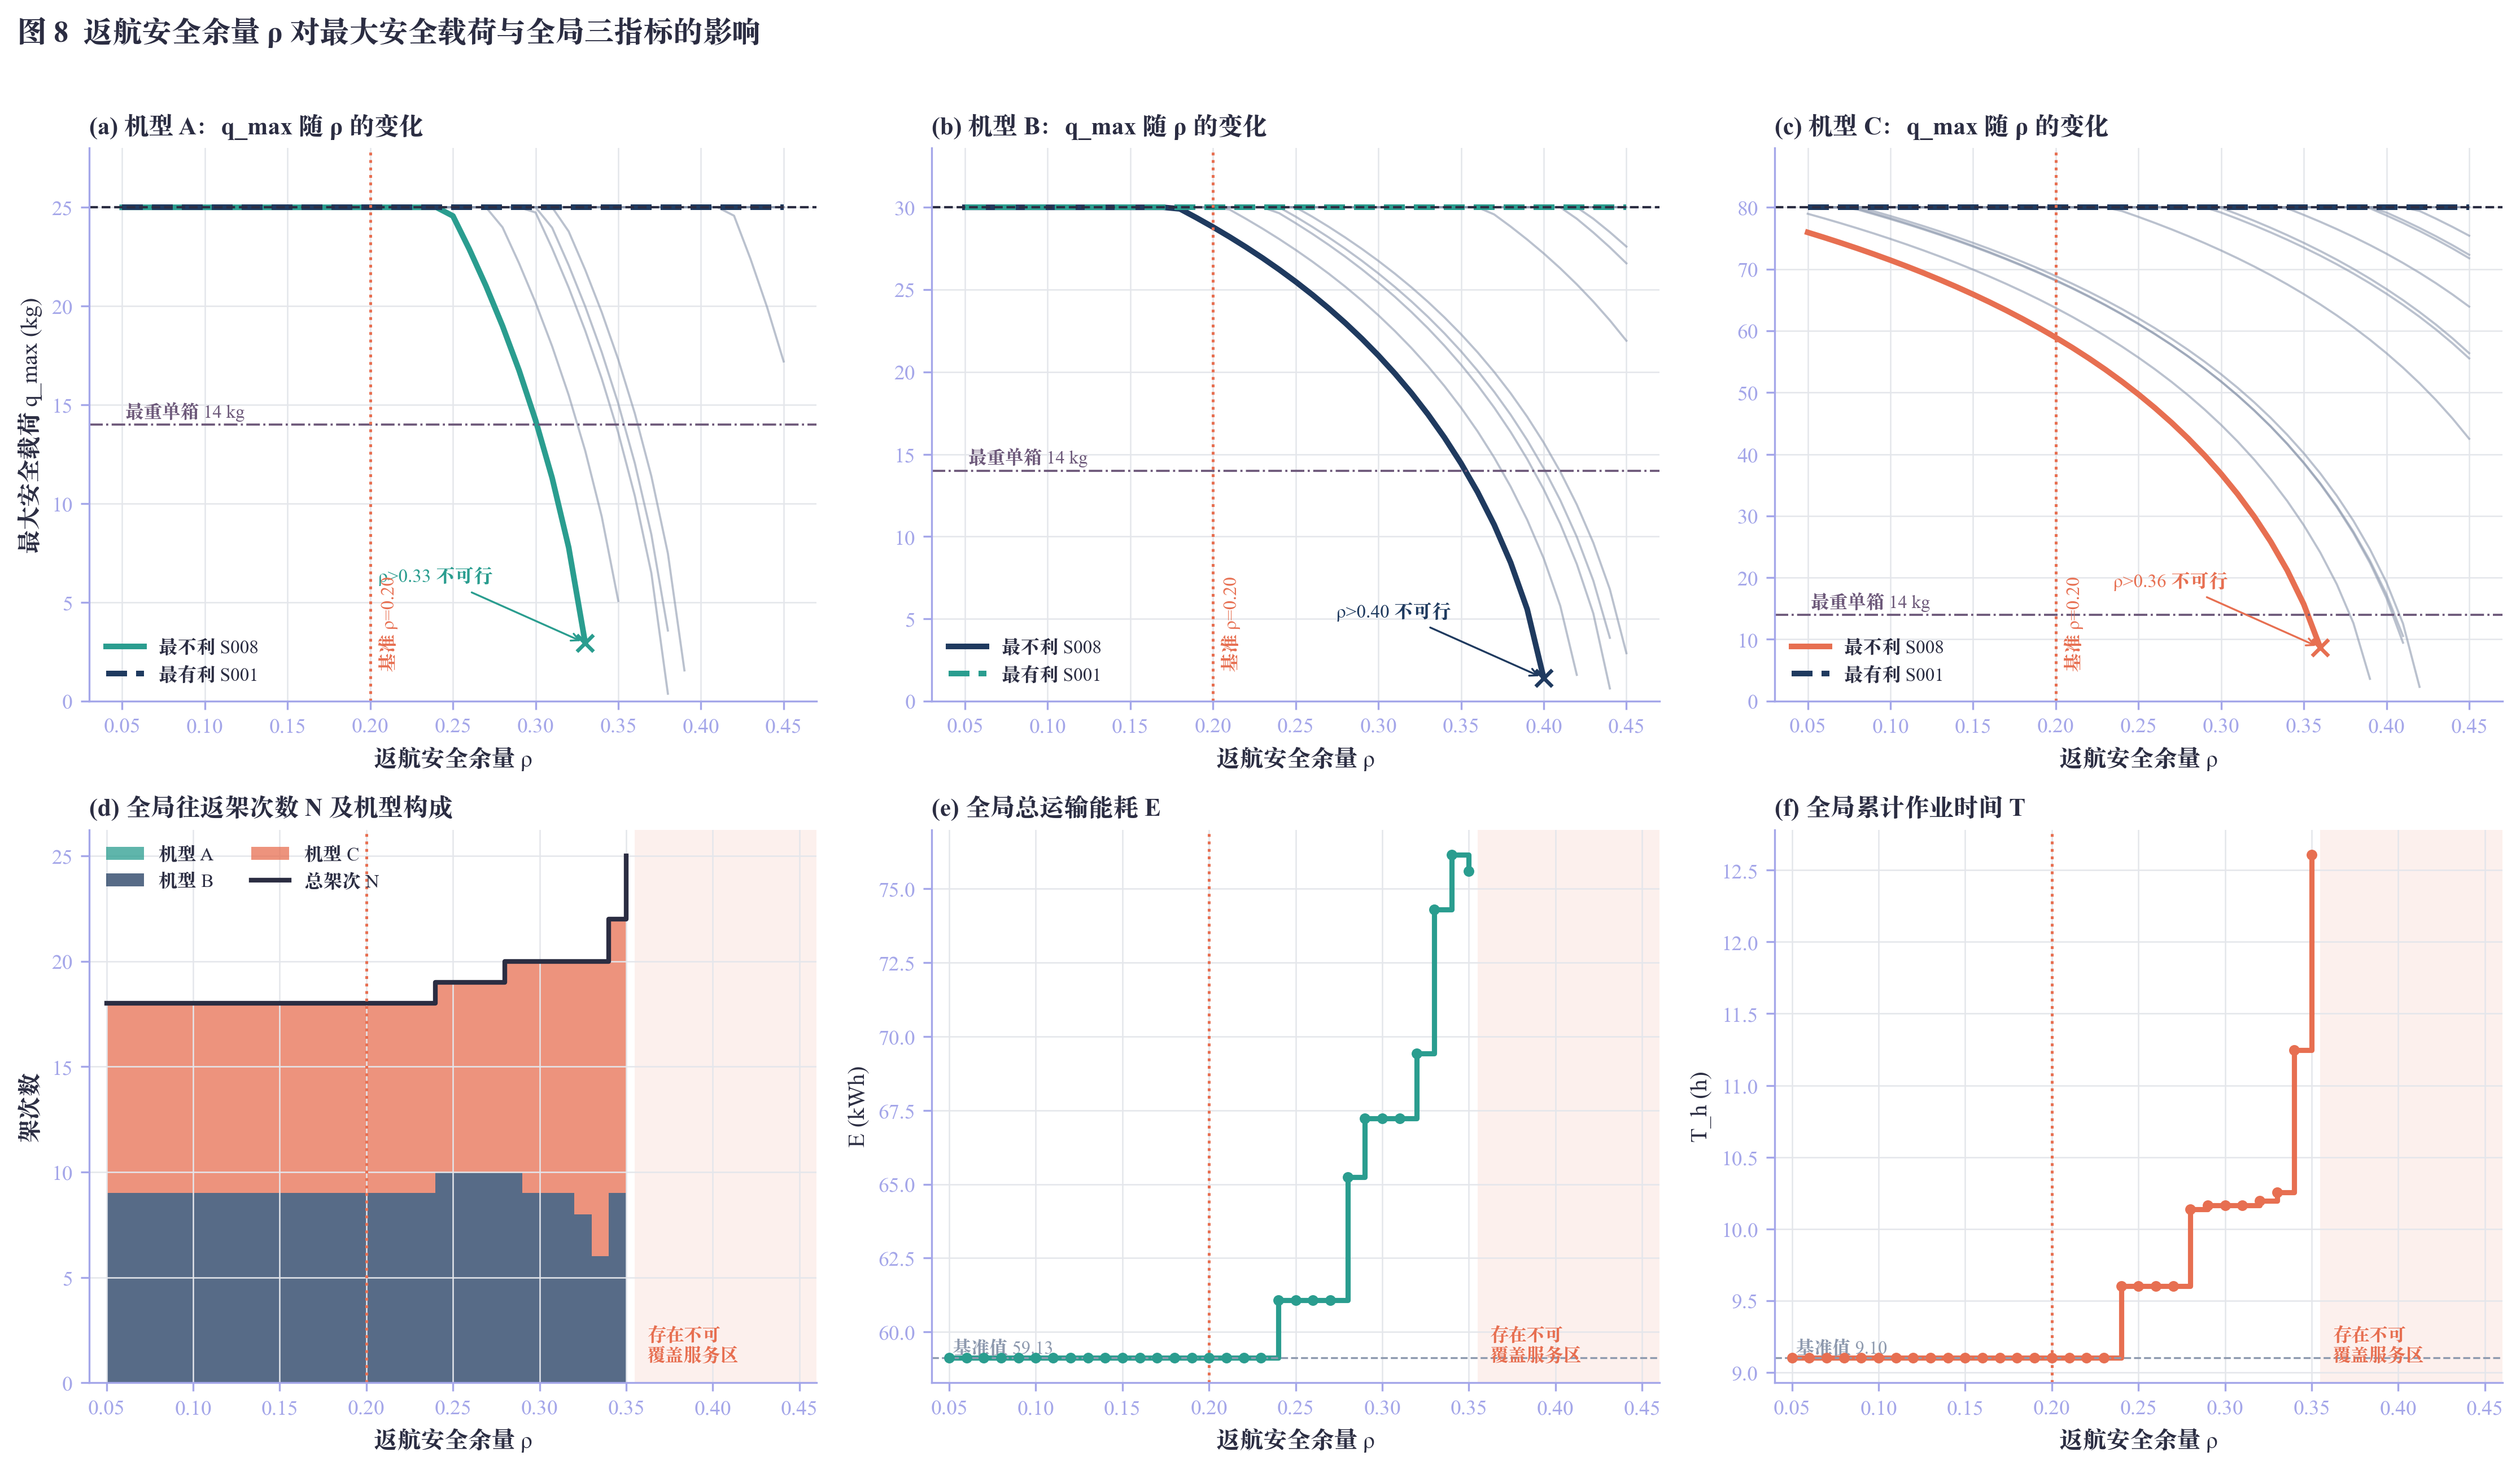
\includegraphics[width=\linewidth]{figures/Q1/图08_敏感性_载荷与三指标.png}
\caption{返航安全余量对最大安全载荷及全局架次、能耗和时间的影响}
\label{fig:q1-rho-sensitivity}
\end{figure}

\begin{figure}[H]
\centering
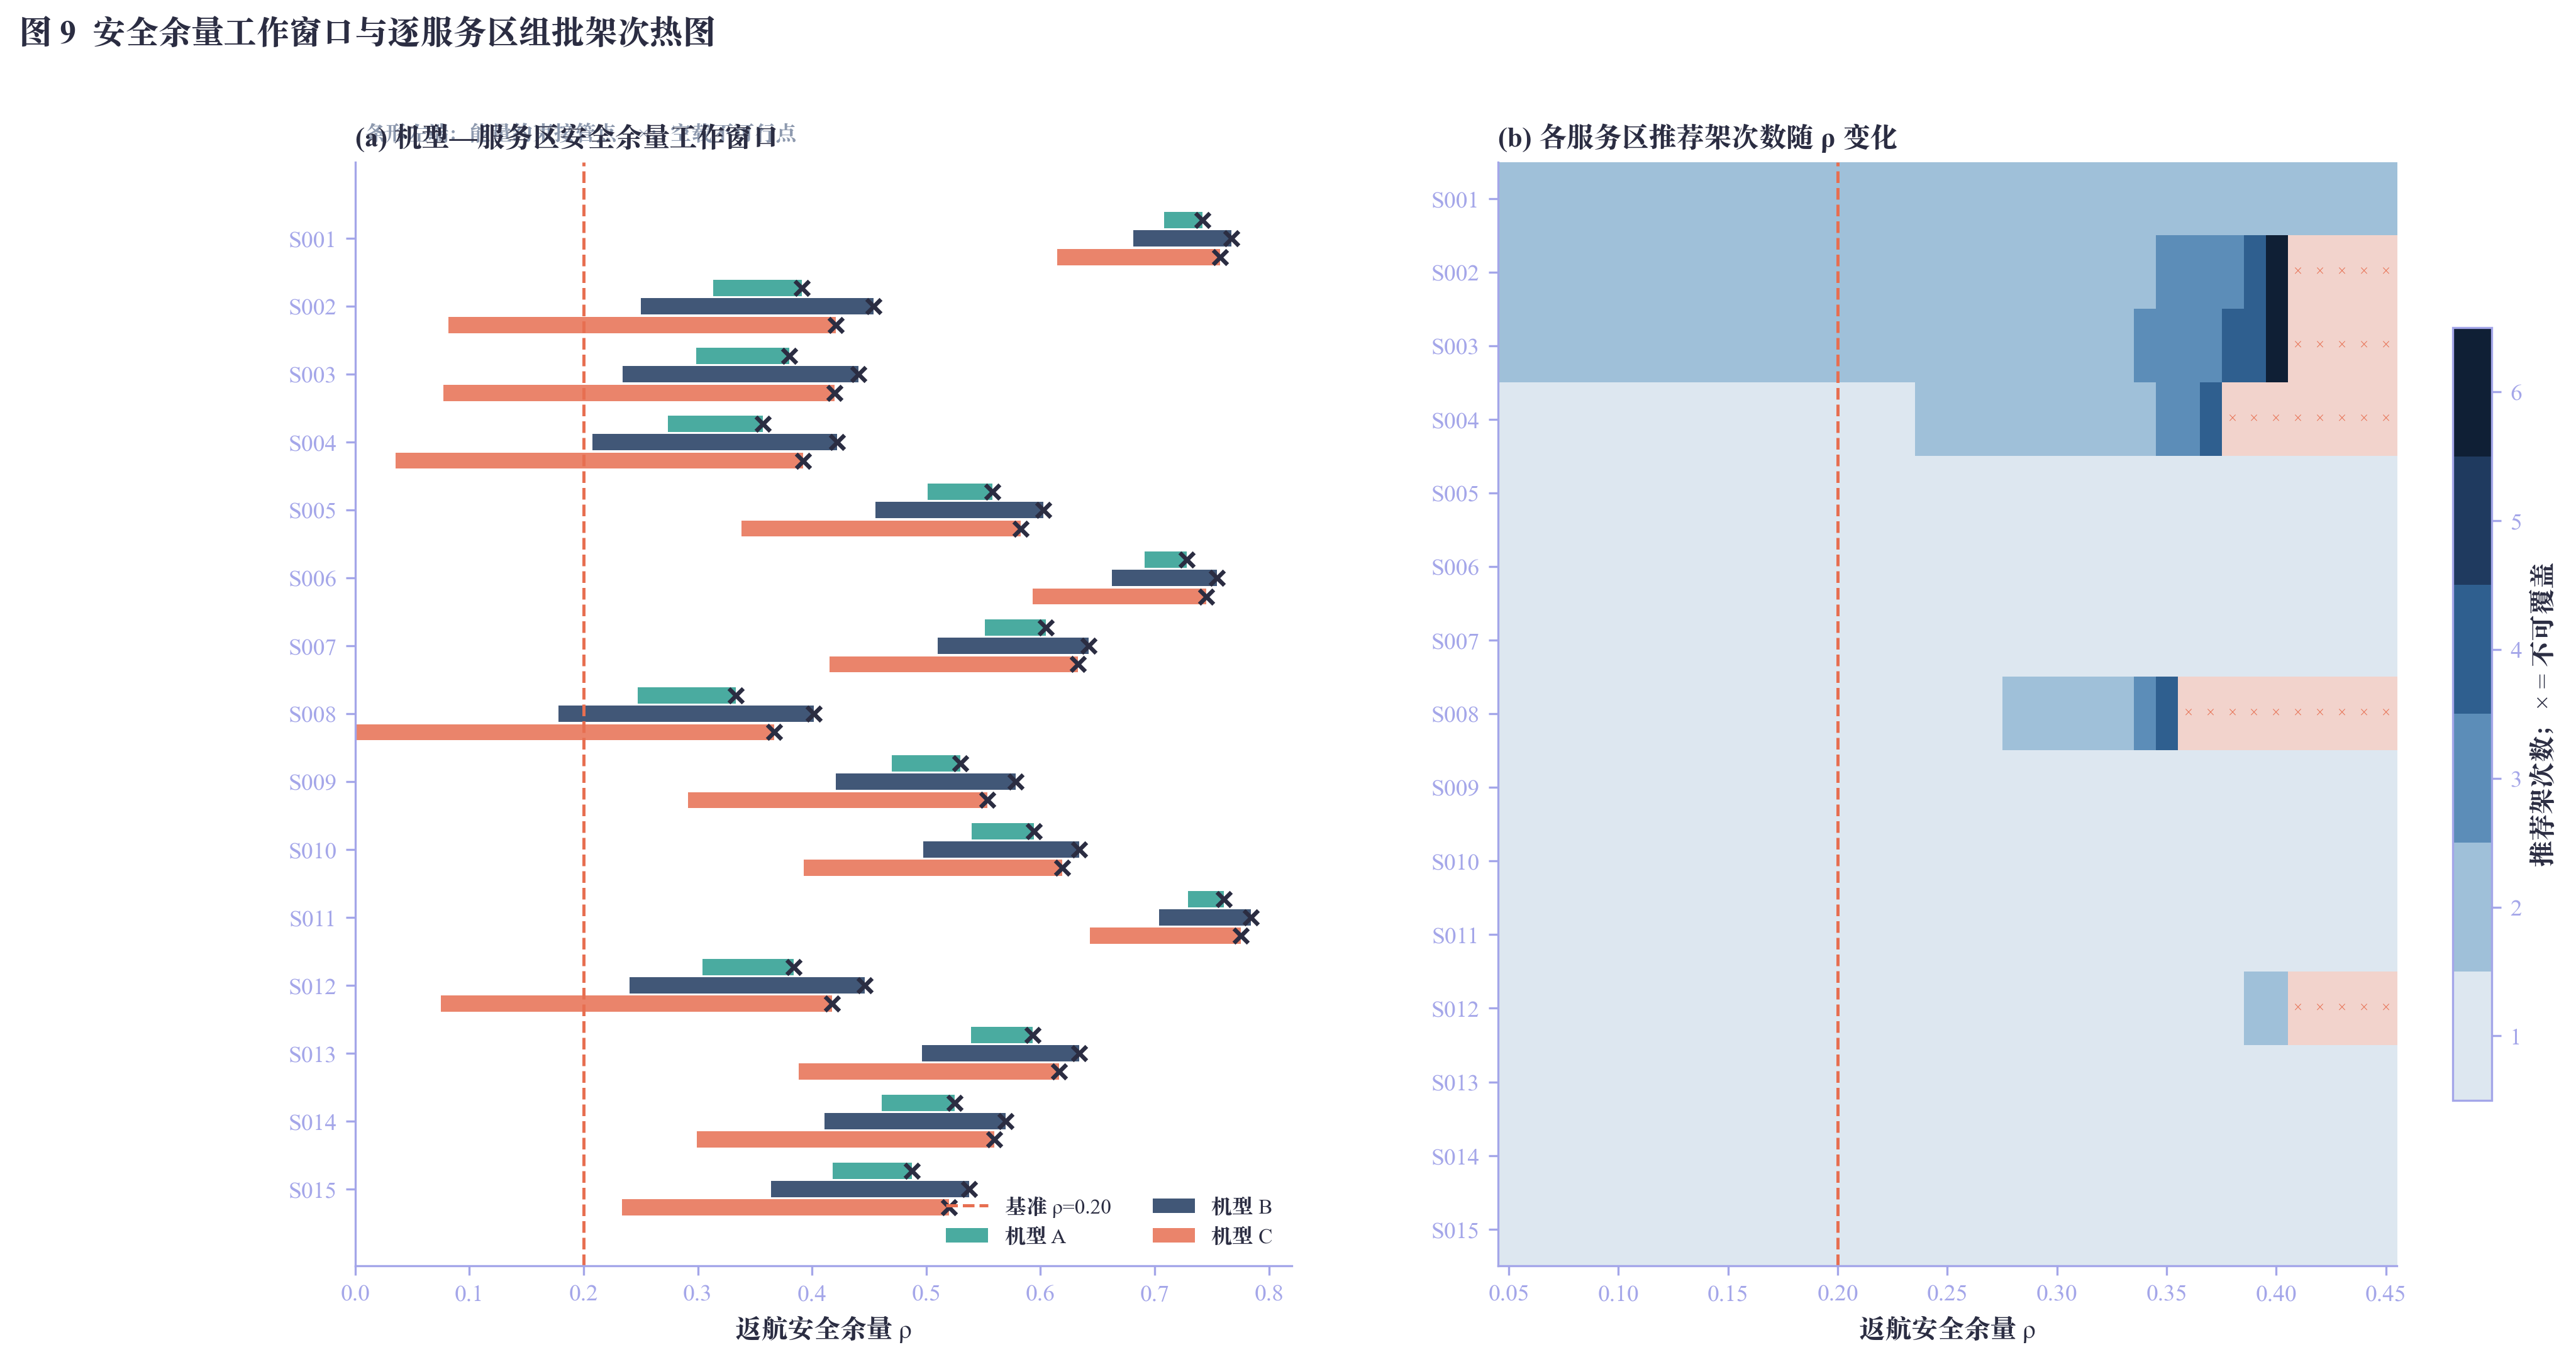
\includegraphics[width=\linewidth]{figures/Q1/图09_安全余量工作窗口与架次热图.png}
\caption{返航安全余量变化下各服务区推荐架次数}
\label{fig:q1-rho-window}
\end{figure}

% 第7章
\clearpage
\section{问题二：异构无人机多点多架次运输调度模型}

\subsection{问题分析}

问题二在问题一的航段几何、载荷—航程及能耗口径上，进一步联合决定货箱组批、服务区访问顺序、无人机与电池分配及架次开始时刻。与单点模型相比，多点架次利用服务区间直飞减少重复往返，但须同时满足逐箱时限、机体互斥和电池充满后再用等约束。本文以整数规划描述该组合优化问题，再用自适应大邻域搜索与列表调度解码器求取可行方案。

\subsection{多点架次的时间轴、送达时刻与电池周转}

设架次 $p$ 的路线为
\[
i_0=O01\to i_1\to\cdots\to i_K\to i_{K+1}=O01,
\]
其中 $i_1,\ldots,i_K$ 为互异服务区。每条航段按式~\eqref{eq:cruise-altitude}确定地形净空；机型 $g$ 在航段 $(i,j)$ 的飞行时间为
\begin{equation}
\tau_{gij}=\frac{h_{ij}^{+}}{v_g^\uparrow}
+\frac{d_{ij}}{v_g^c}
+\frac{h_{ij}^{-}}{v_g^\downarrow}.
\label{eq:q2-leg-time}
\end{equation}
起飞载荷记为 $q_{p,0}$。在第 $r$ 个服务区卸下质量 $M_{p,r}$ 后，后续航段载荷递减为
\[
q_{p,r}=q_{p,r-1}-M_{p,r},\qquad r=1,\ldots,K.
\]
沿用问题一的等效航程函数，单段能耗及架次能耗为
\begin{equation}
E_{gij}(q)=\frac{d_{ij}E_g^{\mathrm{use}}}{L_g(q)}
+\frac{(m_g^0+q)g_0h_{ij}^{+}}{\eta_g^\uparrow\,3.6\times10^6},
\qquad
E_p=\sum_{r=0}^{K}E_{g,i_r i_{r+1}}(q_{p,r}),
\quad
E_p\le(1-\rho_g)E_g^{\mathrm{use}} .
\label{eq:q2-leg-energy}
\end{equation}
各架次从 O01 起飞前经历固定准备及逐箱装载；每个服务区各经历一次基础交接，每箱再增加交接时间。设 $n_p$ 为架次箱数，第 $r$ 个服务区内货箱 $b$ 的交接顺序为 $j$，则其相对架次开始时刻的送达偏移为
\begin{equation}
\delta_{bp}=t_g^{\mathrm{prep}}+n_p t_g^{\mathrm{load}}
+\sum_{\ell=1}^{r}\tau_{g,i_{\ell-1}i_\ell}
+t_g^{\mathrm{hand}}+j t_g^{\mathrm{box}} .
\label{eq:q2-delivery-offset}
\end{equation}
同一服务区内优先交付硬时限较早的货箱，其次按应急优先系数由高到低排序。架次结束时刻包含全部航段、准备、装载及交接时间。架次耗能后的电池荷电状态为 $s_p=1-E_p/E_g^{\mathrm{use}}$；共享电池再次使用前须充至 $100\%$。按题目给定的快慢充时间比例，电池从荷电状态 $s$ 充满的时间为
\begin{equation}
t_g^{\mathrm{chg}}(s)=
\begin{cases}
T_g^{\mathrm{full}}\left[0.65(0.9-s)/0.9+0.35\right],&s<0.9,\\
T_g^{\mathrm{full}}\,0.35(1-s)/0.1,&s\ge0.9.
\end{cases}
\label{eq:q2-charge-time}
\end{equation}
同型电池可在同型无人机间周转；无人机返场后可执行下一架次，电池则须完成充电后方可复用。

\subsection{及时性指标与四指标量化}

记 $t_b=t_p^{\mathrm{st}}+\delta_{bp}$ 为货箱送达时刻，$t_b^{\mathrm{exp}}$ 为期望送达时刻，$w_b$ 为应急优先系数。以优先加权平均迟到 $\bar L$ 和优先加权平均送达时刻 $\bar D$ 衡量及时性：
\begin{equation}
\bar L=\frac{\sum_b w_b(t_b-t_b^{\mathrm{exp}})_+}{\sum_b w_b},
\quad
\bar D=\frac{\sum_b w_bt_b}{\sum_b w_b},
\quad
f_T=\frac{\bar L+0.1\bar D}{3600}.
\label{eq:q2-timeliness}
\end{equation}
其中 $\bar L$ 为主要时效量，$\bar D$ 用于区分迟到程度相近或均未迟到的方案。另定义完工时间、总能耗和架次数为
\[
f_M=\frac{\max_p t_p^{\mathrm{en}}}{3600},
\qquad
f_E=\sum_pE_p,
\qquad
f_N=|P|.
\]
医疗物资须在期望送达时刻前送达，首批保障货箱须在首批截止时刻前送达；其余货箱的期望时刻只参与 $f_T$。搜索阶段使用归一化加权和，并对硬时限迟到施加罚项：
\begin{equation}
F=w_Tf_T+w_Mf_M+w_E\frac{f_E}{50}+w_N\frac{f_N}{20}
+100\sum_{b\in B^{\mathrm{hard}}}\frac{(t_b-\bar t_b)_+}{3600}
+5\sum_{b\in B^{\mathrm{hard}}}\mathbf{1}(t_b>\bar t_b).
\label{eq:q2-scalar-objective}
\end{equation}
其中 $B^{\mathrm{hard}}$ 为硬时限货箱集合，$\bar t_b$ 为其截止时刻。推荐权重为
\[
(w_T,w_M,w_E,w_N)=(3,1.5,1,0.5),
\]
体现时效优先，其次为完工时间、能耗和架次数。

\subsection{整数规划表述与求解框架}

令 $x_{bp}\in\{0,1\}$ 表示货箱 $b$ 是否装入架次 $p$，$y_{pij}\in\{0,1\}$ 表示架次是否经过航段 $i\to j$，$z_{pu}$ 和 $\zeta_{pk}$ 分别表示无人机 $u$ 与电池 $k$ 是否执行架次 $p$。路线从 O01 出发并回到 O01，且只访问装有对应货箱的服务区。其多目标整数规划形式为
\begin{equation}
\begin{aligned}
\min\quad &(f_T,f_M,f_E,f_N),\\
\text{s.t.}\quad
&\sum_p x_{bp}=1,\qquad \forall b,\\
&\sum_b m_bx_{bp}\le Q_{g(p)},\quad
  \sum_b v_bx_{bp}\le V_{g(p)},\qquad \forall p,\\
&E_p\le(1-\rho_{g(p)})E_{g(p)}^{\mathrm{use}},\qquad \forall p,\\
&t_b=t_p^{\mathrm{st}}+\delta_{bp},\quad
  t_b\le \bar t_b,\qquad \forall b\in B^{\mathrm{hard}},\\
&\text{同一无人机的架次不重叠；同一电池须在充满后再用},\\
&x_{bp},y_{pij},z_{pu},\zeta_{pk}\in\{0,1\}.
\end{aligned}
\label{eq:q2-integer-model}
\end{equation}
该问题同时包含组批、路线、异构资源与时间窗决策。本文不将该整数规划的形式化表述误作精确求解结果；实际求解采用下述启发式框架，并由解码器显式排定资源和检查时间窗。

\subsection{列表调度解码器与自适应大领域搜索}

给定组批和访问顺序后，先按硬时限最迟开始时刻排序；无硬时限架次再按期望送达时刻排序。解码器依次选择同型中最早可用的无人机和电池，架次开始时刻取两种资源的可用时刻较晚者；电池可用时刻更新为本架次返场并充满后的时刻。该规则保证无人机任务不重叠、电池任务与充电不重叠，初始资源均位于 O01 且电池满电。

ALNS 从问题一式的单点组批方案出发，每次迭代移除 4--12 个货箱，再用贪心或带噪声的贪心插入到已有架次、路线停靠点或新架次。五类破坏算子分别执行随机移除、最迟送达移除、同区移除、整架次移除和末班架次移除；模拟退火准则决定是否接受新解，并每 100 次迭代按算子近期表现更新其抽取权重。修复过程中只保留满足载质量、体积、能量和服务区归属约束的架次；最多五个停靠点的访问顺序通过枚举重排，并以小概率尝试更换机型。主搜索运行 8000 次迭代并作 4000 次架次顺序交换精修；随后对及时性、完工时间、能耗和架次数分别加强权重，各运行 3000 次，以比较不同偏好下的可行方案。图~\ref{fig:q2-alns}展示主搜索的目标收敛、算子权重自适应及指标变化。

\begin{figure}[H]
\centering
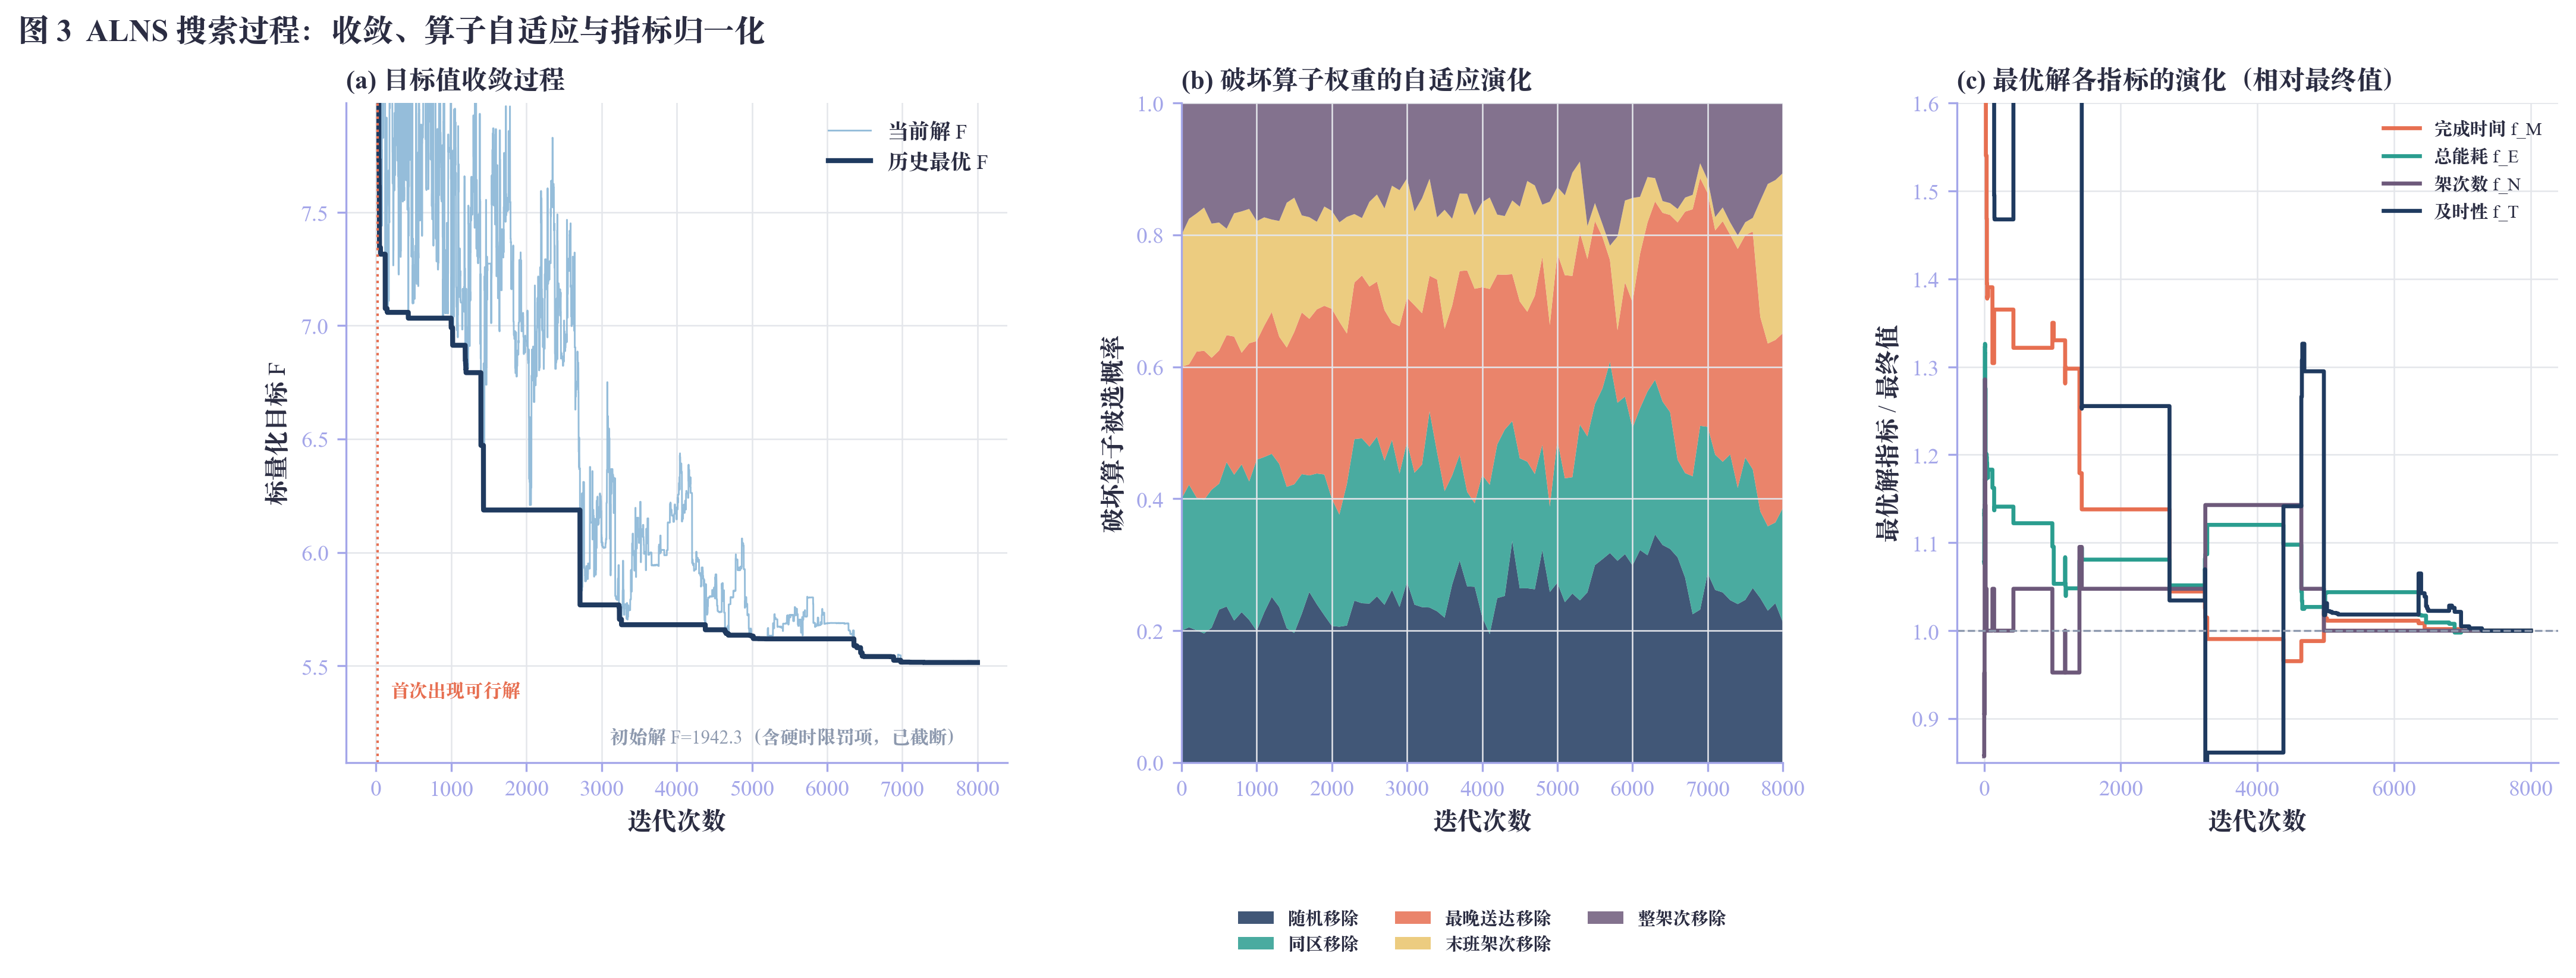
\includegraphics[width=\linewidth]{figures/Q2/图03_ALNS搜索过程.png}
\caption{ALNS 搜索收敛、算子权重自适应与指标演化}
\label{fig:q2-alns}
\end{figure}

\subsection{推荐方案与结果分析}

推荐权重下，从主搜索及四种偏好搜索记录中选择标量目标 $F$ 最小的可行候选。推荐解来自完工时间优先情景的搜索轨迹，经推荐权重重新评价后 $F=5.239$；该值仅表示已搜索候选中的最好值。方案使用 22 架次（A 型 9 次、B 型 7 次、C 型 6 次），配送 80 箱，完工时间为 $1.977\,\mathrm{h}$，总能耗为 $71.839\,\mathrm{kWh}$。其 $f_T=0.0955$，优先加权平均迟到为 $49.259\,\mathrm{s}$、优先加权平均送达时刻为 $2945.615\,\mathrm{s}$。80 箱中有 2 箱晚于期望时刻；31 箱硬时限均满足，最小提前量为 $5.5\,\mathrm{min}$。图~\ref{fig:q2-plan}给出 22 个架次的空间航线，图~\ref{fig:q2-gantt}展示无人机与共享电池的调度时序；逐箱送达时刻和电池荷电状态分别见图~\ref{fig:q2-delivery}和图~\ref{fig:q2-soc}。

\begin{figure}[H]
\centering
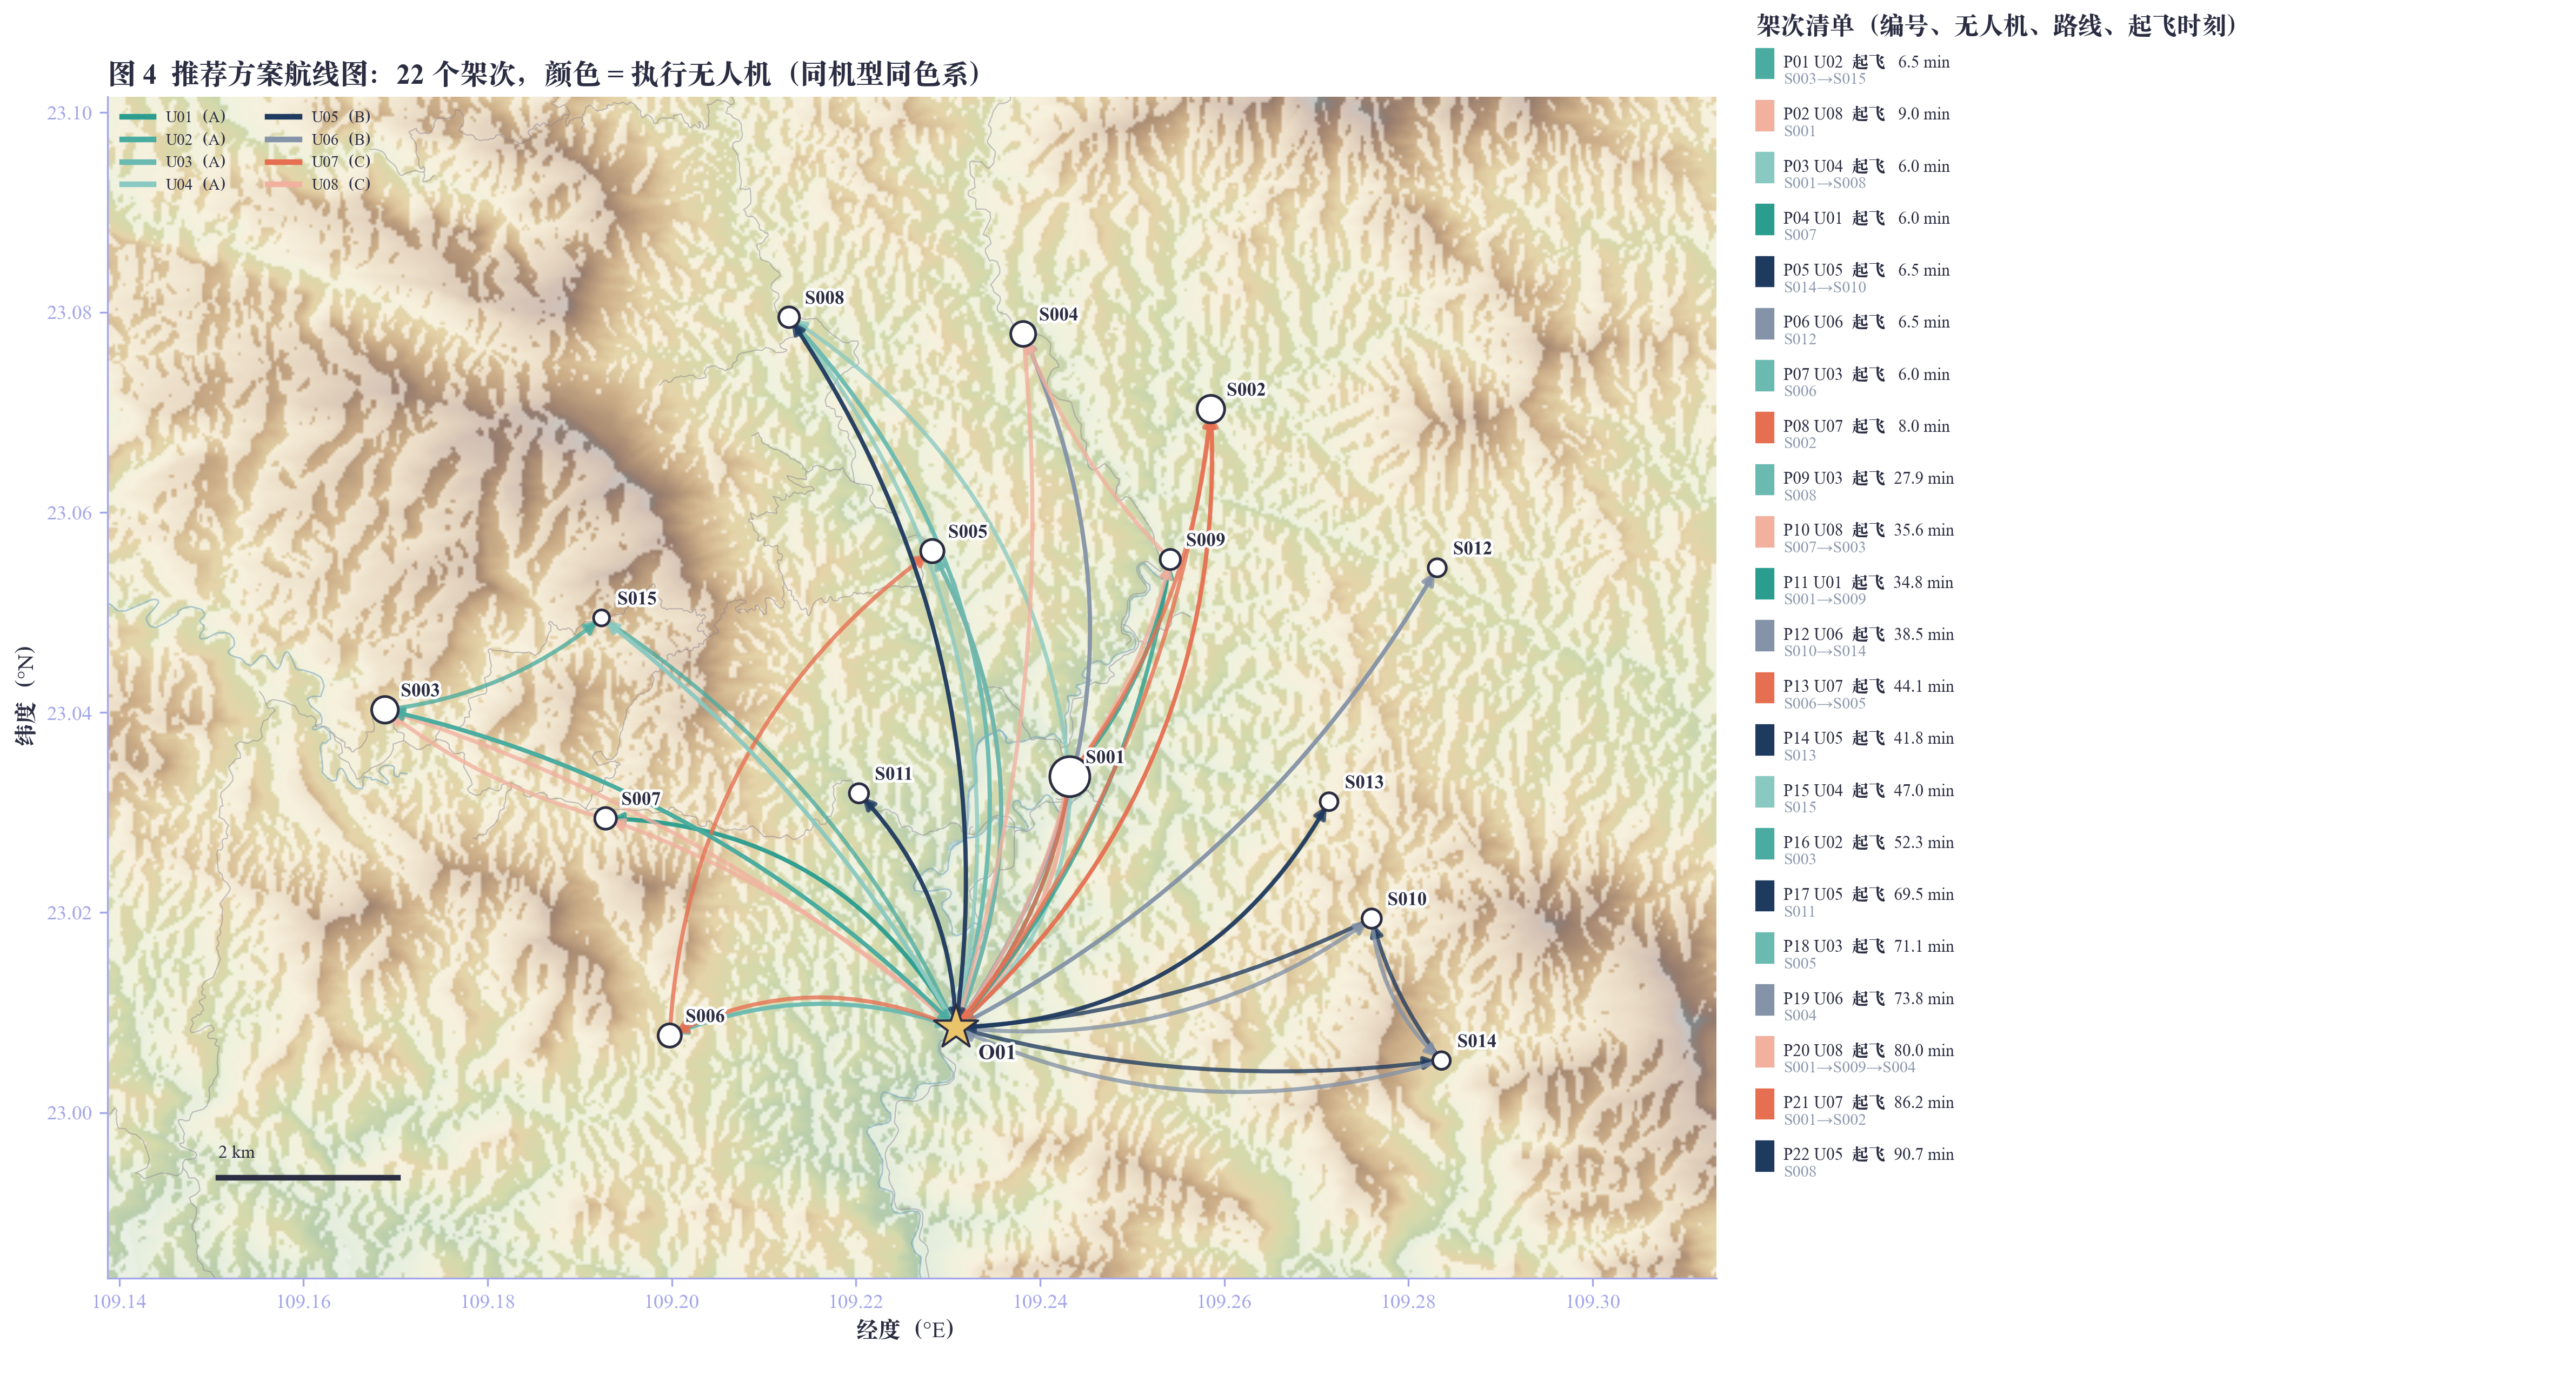
\includegraphics[width=\linewidth]{figures/Q2/图04_推荐方案航线图.png}
\caption{推荐方案的 22 架次多点运输航线}
\label{fig:q2-plan}
\end{figure}

\begin{figure}[H]
\centering
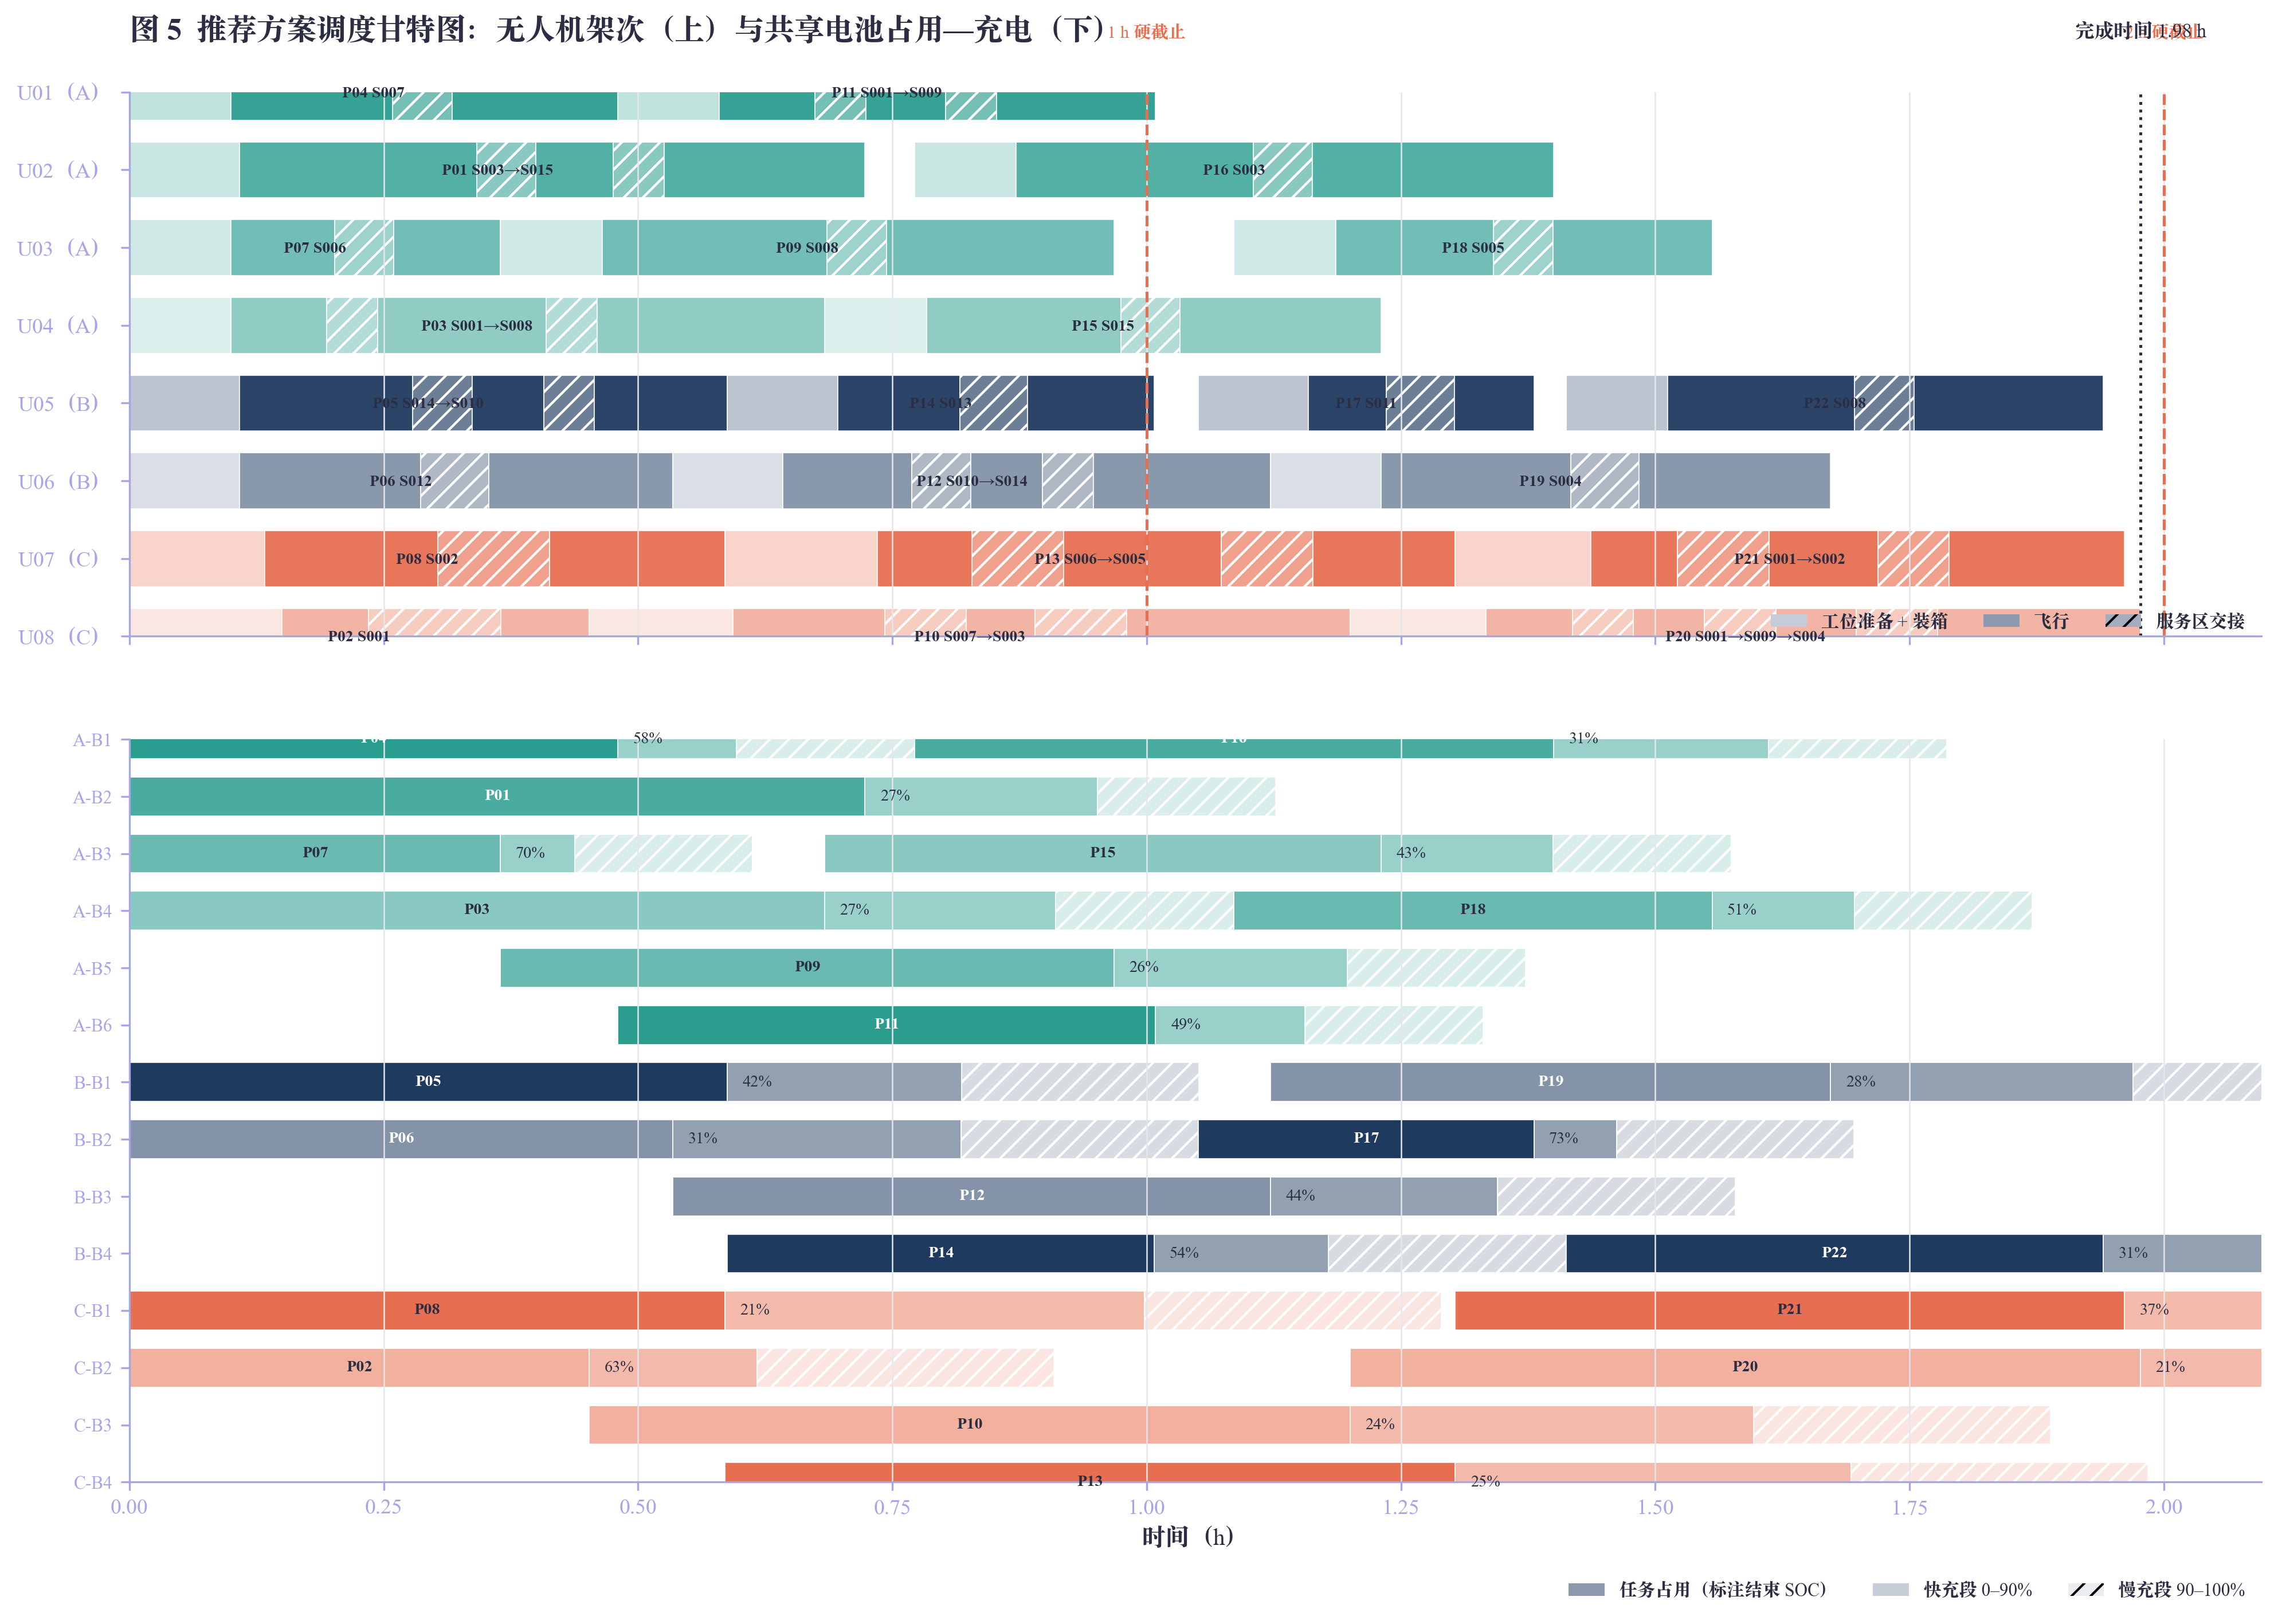
\includegraphics[width=\linewidth]{figures/Q2/图05_调度甘特图.png}
\caption{推荐方案的无人机架次与共享电池调度时序}
\label{fig:q2-gantt}
\end{figure}

\begin{figure}[H]
\centering
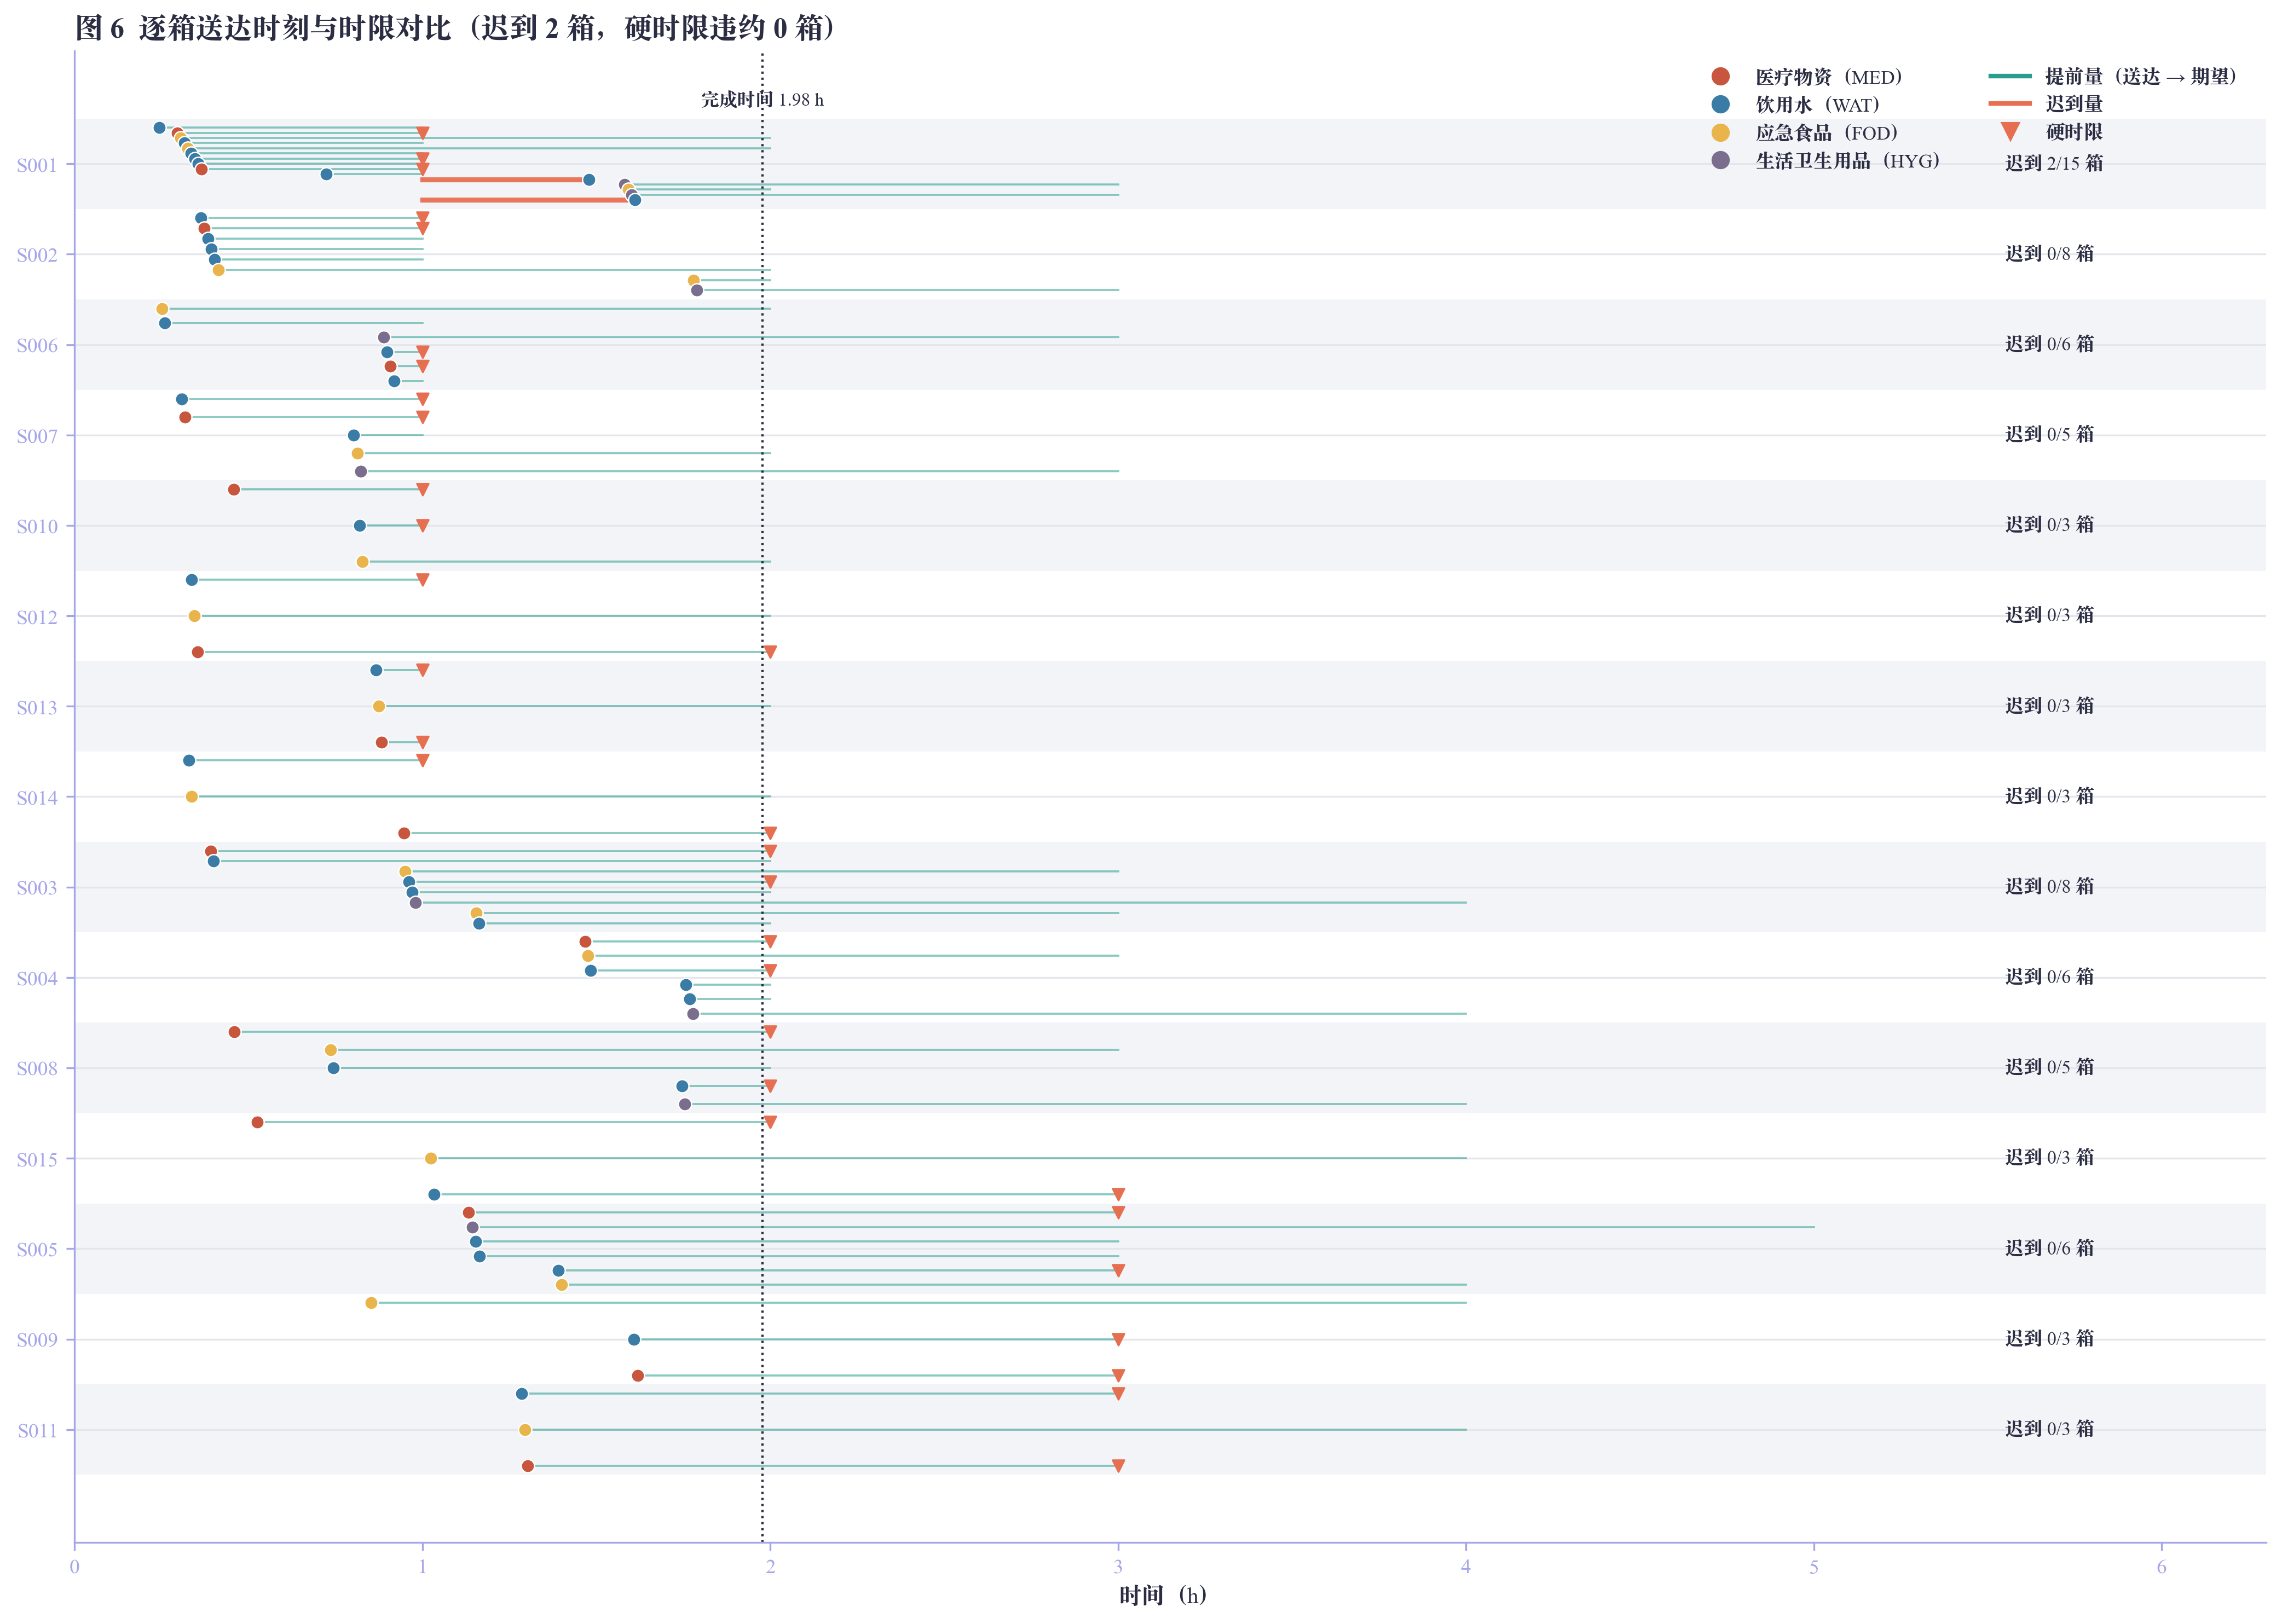
\includegraphics[width=\linewidth]{figures/Q2/图06_逐箱送达时刻.png}
\caption{逐箱送达时刻与期望时限、硬时限的对照}
\label{fig:q2-delivery}
\end{figure}

\begin{figure}[H]
\centering
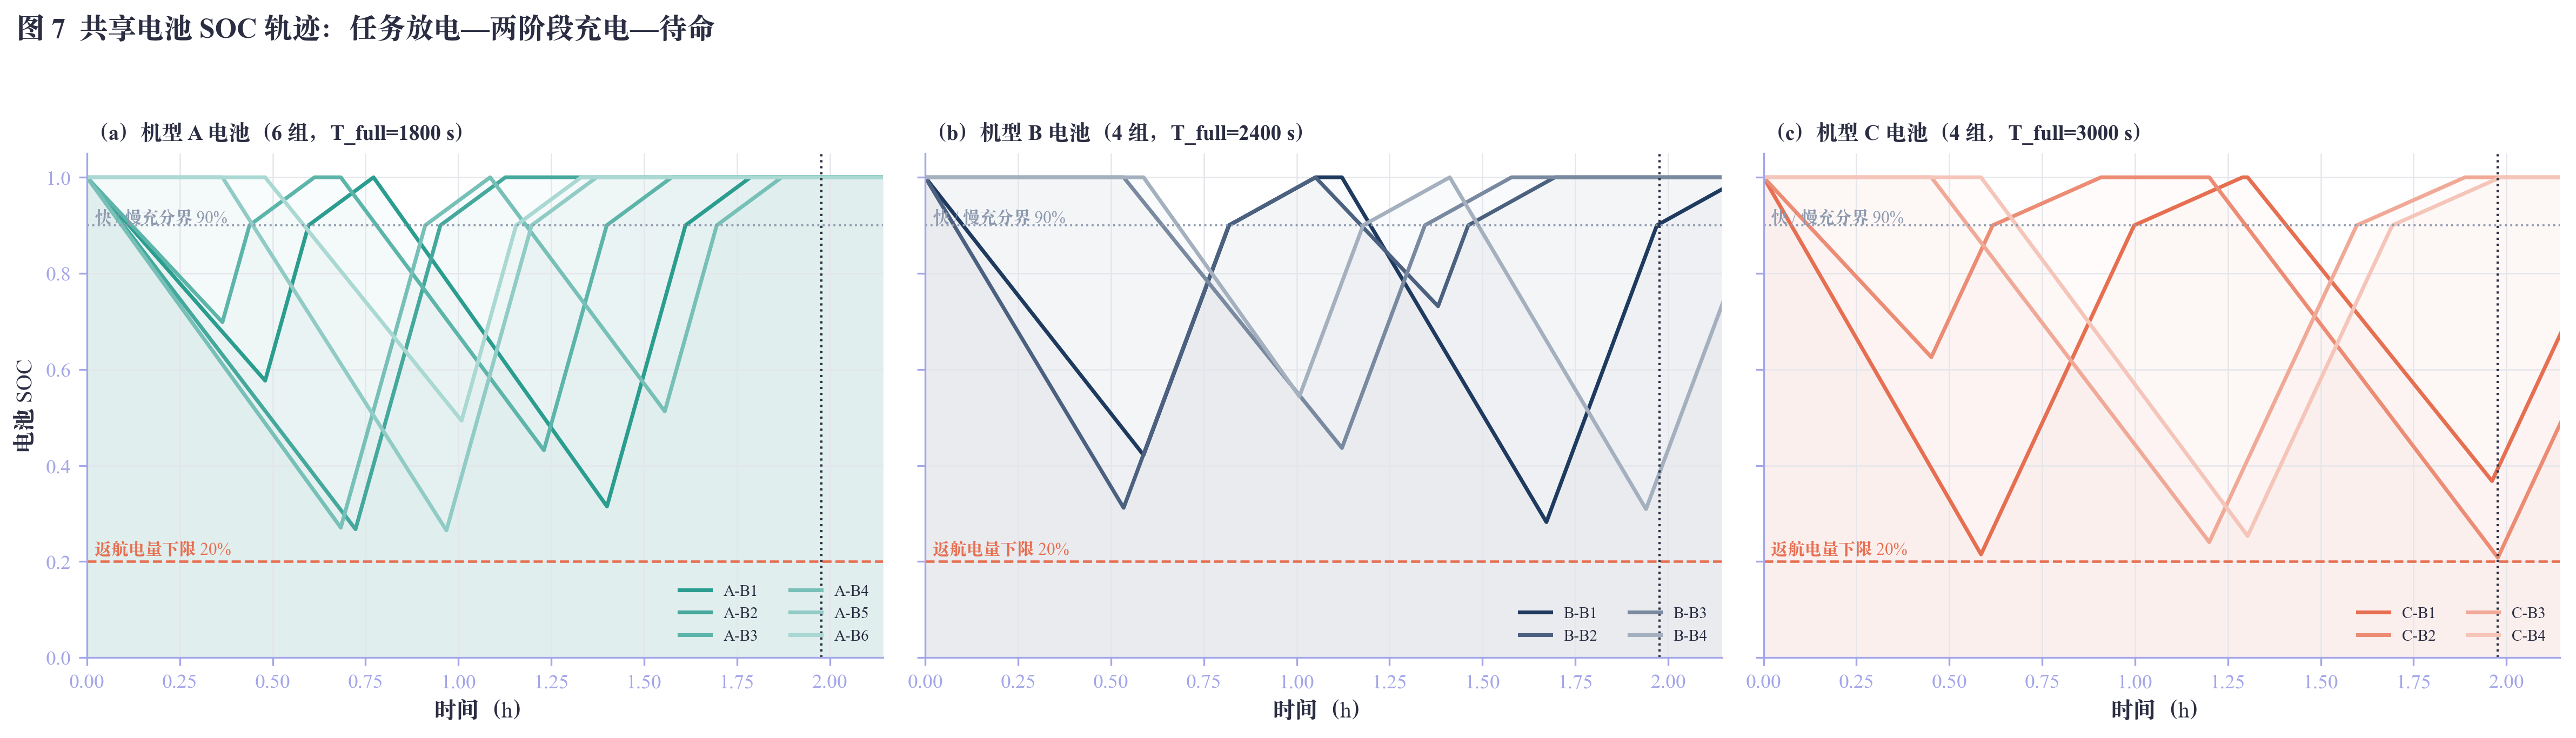
\includegraphics[width=\linewidth]{figures/Q2/图07_电池SOC轨迹.png}
\caption{共享电池任务放电、两阶段充电及待命荷电状态}
\label{fig:q2-soc}
\end{figure}

\subsection{四指标权衡与可行性检验}

表~\ref{tab:q2-tradeoff}比较推荐权重和四种偏好权重下的已搜索方案。及时性指标 $f_T$ 越小越好。能耗优先方案将能耗降至 $63.562\,\mathrm{kWh}$，但完工时间增至 $2.655\,\mathrm{h}$；架次优先方案以 17 架次完成任务，但 $f_T$ 增至 $0.228$、完工时间为 $2.938\,\mathrm{h}$。搜索记录包含 7080 个不同可行解，其中 93 个为记录集内的四指标非支配解；该记录集不是完整可行域，不能据此声称得到全局 Pareto 前沿。图~\ref{fig:q2-tradeoff}预留候选方案间的指标权衡。

\begin{table}[!htbp]
\centering
\caption{不同权重情景下的运输调度候选方案}
\label{tab:q2-tradeoff}
\scriptsize
\setlength{\tabcolsep}{4pt}
\begin{tabularx}{\textwidth}{@{}Xccccc@{}}
\toprule
情景
& $f_T\downarrow$
& $f_M$（h）$\downarrow$
& $f_E$（kWh）$\downarrow$
& $f_N\downarrow$
& 硬时限违约箱数 \\
\midrule
推荐权重（3, 1.5, 1, 0.5） & 0.096 & 1.977 & 71.839 & 22 & 0 \\
及时性优先 & 0.085 & 2.210 & 72.265 & 22 & 0 \\
完工时间优先 & 0.121 & 1.892 & 72.926 & 23 & 0 \\
能耗优先 & 0.147 & 2.655 & 63.562 & 19 & 0 \\
架次优先 & 0.228 & 2.938 & 69.697 & 17 & 0 \\
\bottomrule
\end{tabularx}
\end{table}

对推荐方案另行逐项核验：每箱恰好配送一次；质量、体积和能量约束均满足；同一无人机无重叠任务；电池充满后再使用且电池数量不超库存；所有架次返航荷电状态不低于 $20\%$；硬时限箱均按时送达；路线均从 O01 出发并返回。八项检查全部通过，最大归一化载荷、体积或能量利用率为 $99.0\%$，最低返航荷电状态为 $20.8\%$。这些结果验证了所报告候选方案的约束可行性，但 ALNS 属于启发式搜索，结果会受到权重与搜索过程影响，尚不能证明全局最优。图~\ref{fig:q2-tradeoff}展示不同权重方案及搜索记录中的非支配候选，图~\ref{fig:q2-resource}则展示无人机和电池资源的占用情况。
\begin{figure}[H]
\centering
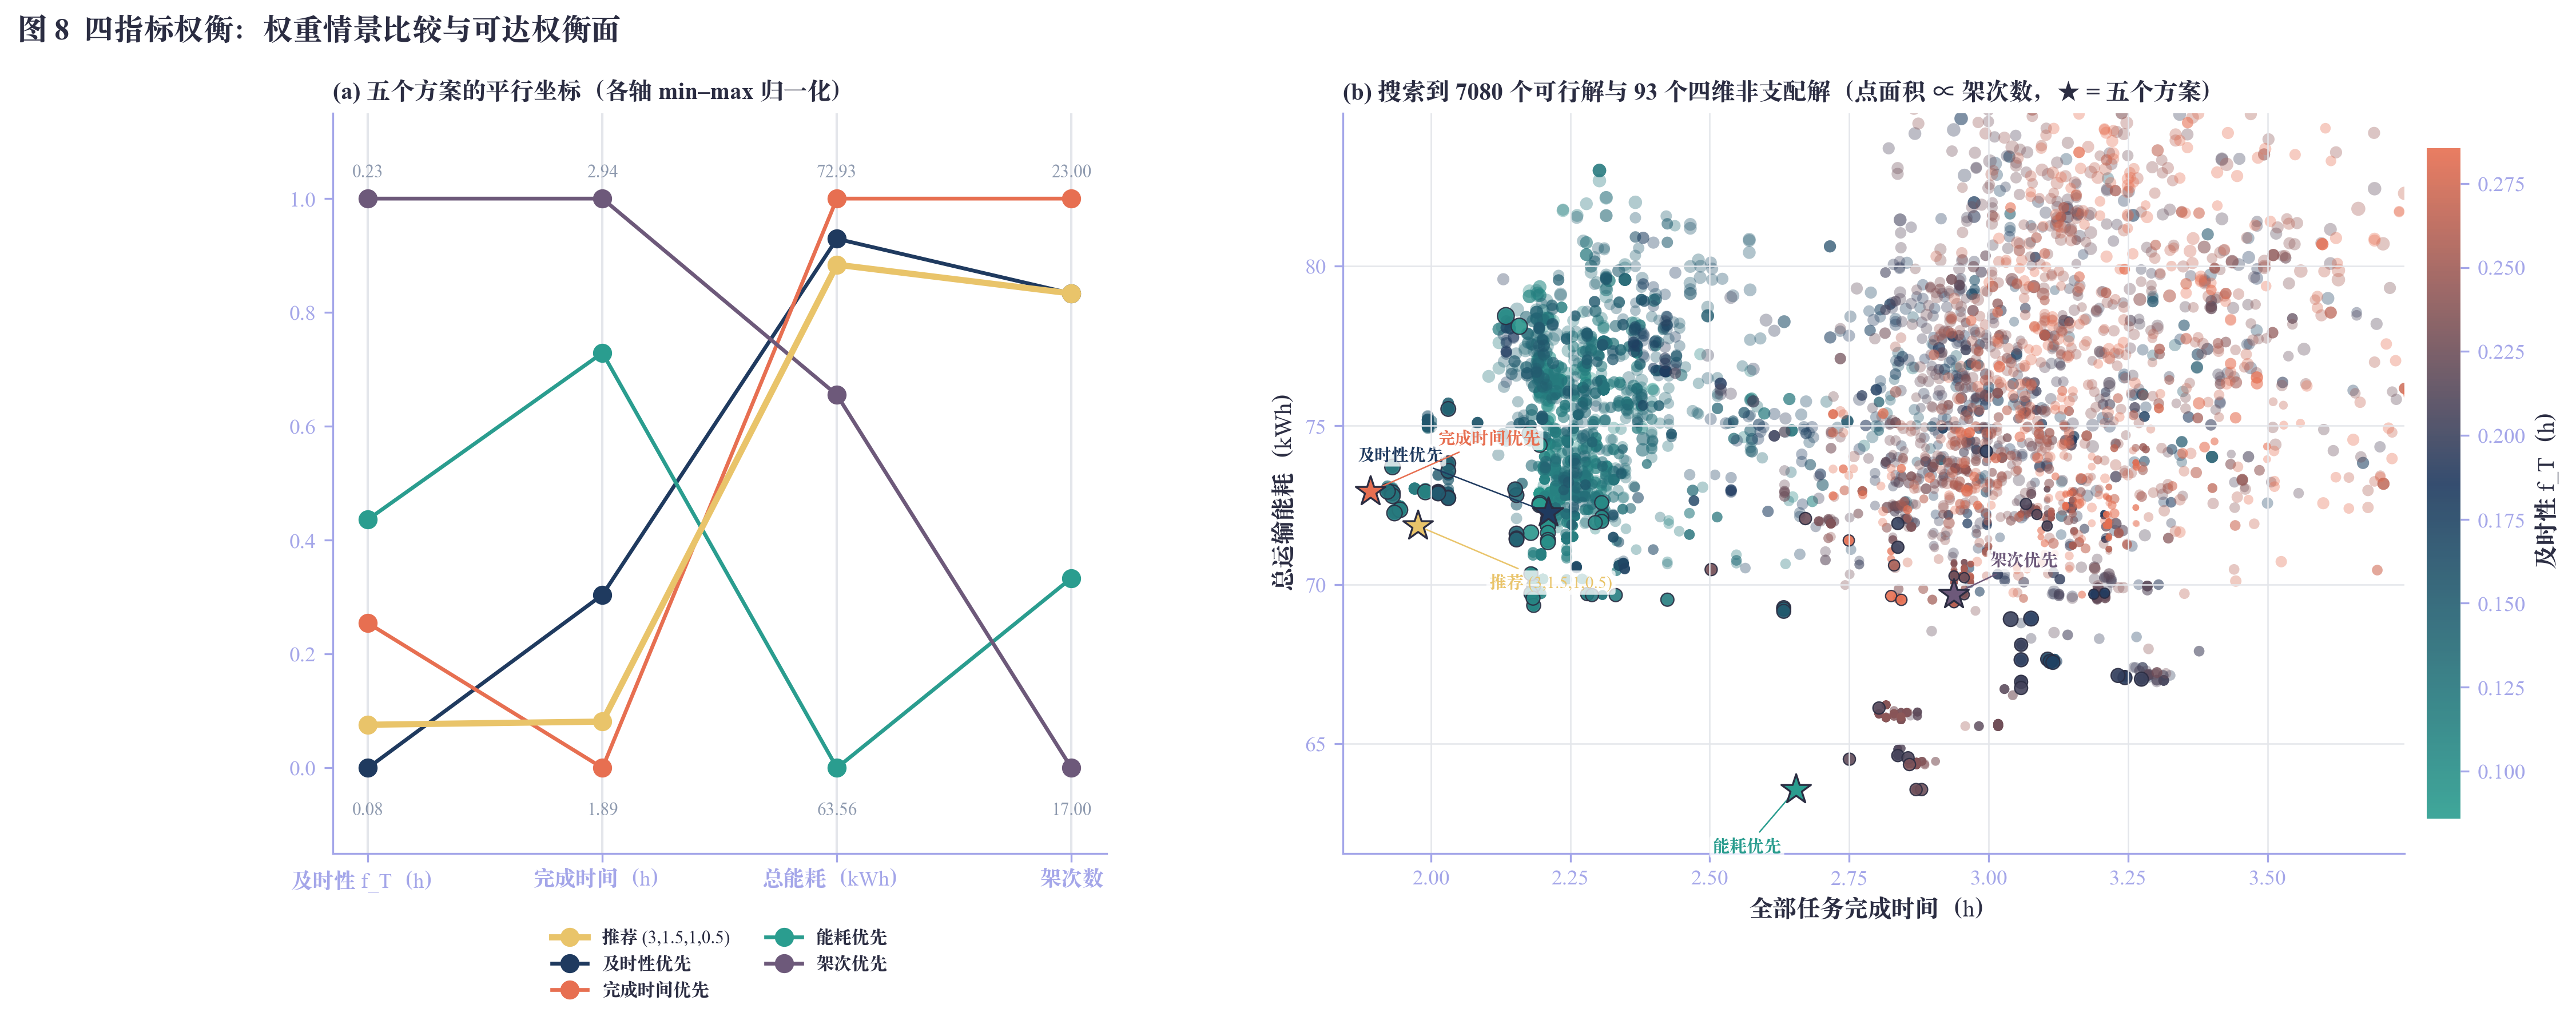
\includegraphics[width=\linewidth]{figures/Q2/图08_指标权衡.png}
\caption{推荐方案与不同偏好候选的四指标权衡}
\label{fig:q2-tradeoff}
\end{figure}

\begin{figure}[H]
\centering
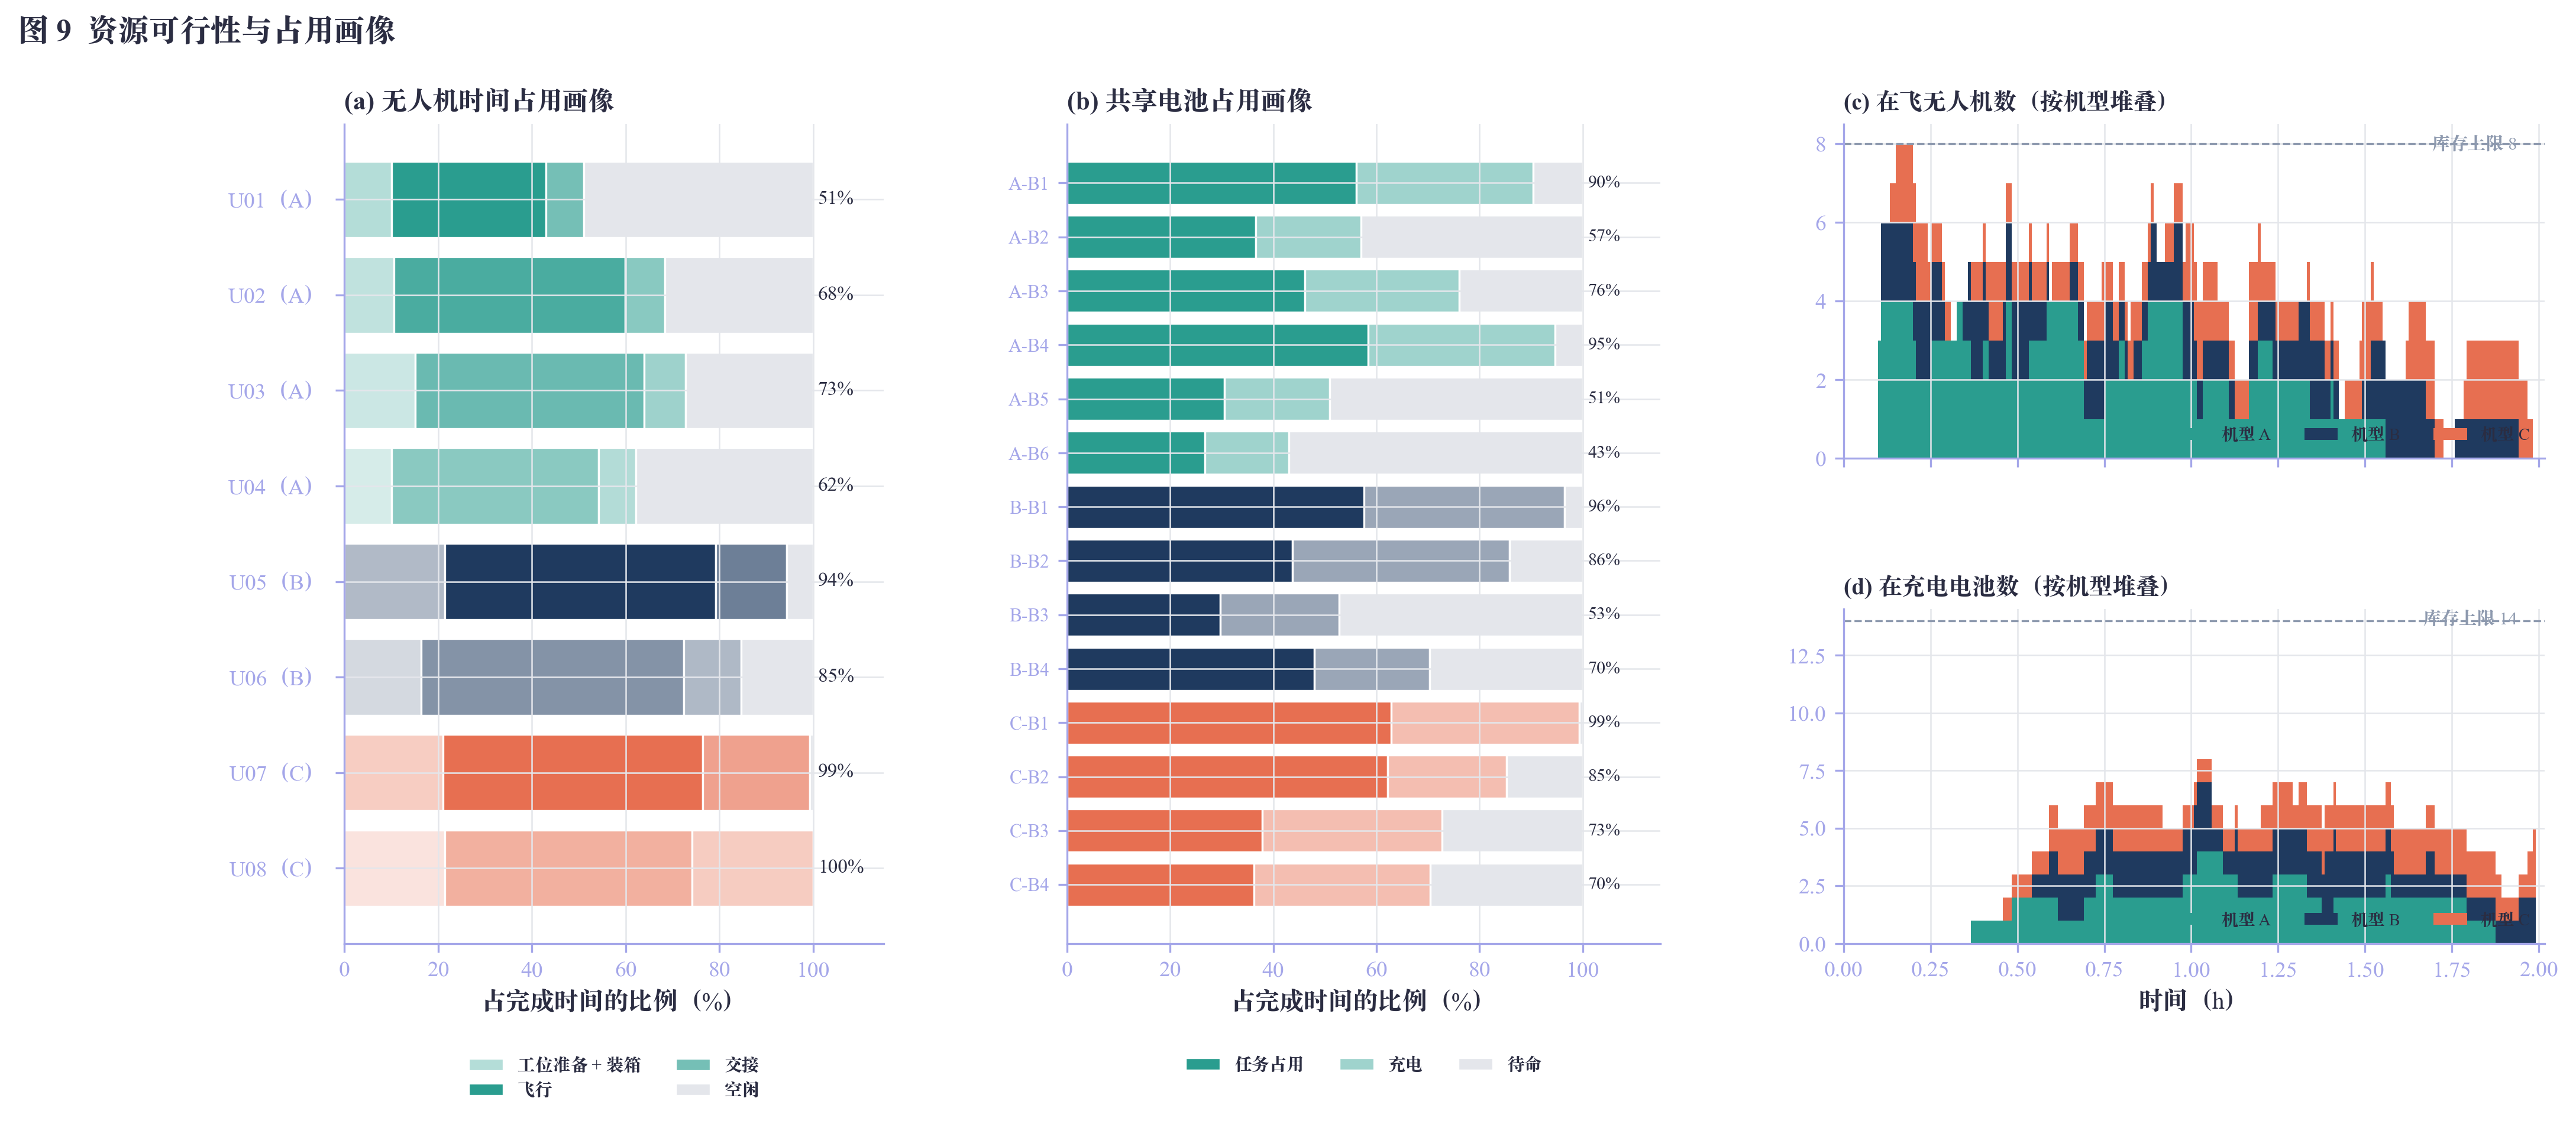
\includegraphics[width=\linewidth]{figures/Q2/图09_资源可行性画像.png}
\caption{推荐方案的无人机与共享电池资源占用画像}
\label{fig:q2-resource}
\end{figure}

% 第8章
\vspace{\baselineskip}
\section{问题三：通信约束下的运输与中继联合调度模型}

\subsection{问题分析}

问题二的运输方案仅考虑配送资源与时间窗，山区遮挡可能使无人机在飞行或服务区交接时失去与 G01 的通信。为满足问题三的全程通信要求，本文保留问题二的货箱、机型、航线、能耗、电池周转及硬时限约束，并新增通信状态、中继站位置和中继任务时序决策。

模型分为空间与时间两层：先依据链路预算和地形视线判定直连盲区，再从候选悬停点中选择能够覆盖盲区且可回传至 G01 的中继站；随后将运输航段及交接期间的中继需求转换为服务区间，与运输无人机、电池和中继无人机联合排程。通信仅允许“运输机--G01”直连或“运输机--中继机--G01”单跳中继，不考虑中继机之间转发。搜索采用问题二的 ALNS 框架，但由解码器同步安排中继资源，并剔除不能实现连续通信的方案。

\subsection{链路预算与覆盖半径}

接收灵敏度为 $-98\,\mathrm{dBm}$，再留取 $8\,\mathrm{dB}$ 链路裕度，故接收门限为 $-90\,\mathrm{dBm}$。按双向链路中较小的允许路径损耗确定可用预算。载频取 $2400\,\mathrm{MHz}$，自由空间损耗及地形遮挡后的路径损耗分别为
\begin{equation}
L_{\mathrm{FSPL}}=32.45+20\log_{10}f_{\mathrm{MHz}}
+20\log_{10}D_{\mathrm{km}}
=100.05+20\log_{10}D_{\mathrm{km}},\qquad
L_{\mathrm{path}}=L_{\mathrm{FSPL}}+10I_{\mathrm{obs}},
\label{eq:q3-path-loss}
\end{equation}
其中 $I_{\mathrm{obs}}=1$ 表示剖面视线被地形遮挡，否则为 $0$。由 $L_{\mathrm{path}}\le L_{\max}$ 得到的等效半径列于表~\ref{tab:q3-link-budget}。这些半径用于链路筛选，实际可用性还取决于地形剖面。

\begin{table}[!htbp]
\centering
\caption{通信链路预算及等效覆盖半径}
\label{tab:q3-link-budget}
\scriptsize
\setlength{\tabcolsep}{5pt}
\begin{tabularx}{\textwidth}{@{}Xccc@{}}
\toprule
链路 & 允许损耗 $L_{\max}$（dB） & 视距半径（km） & 遮挡半径（km） \\
\midrule
运输机--G01 & 122 & 12.51 & 3.96 \\
运输机--中继机 & 116 & 6.27 & 1.98 \\
中继机--G01 & 126 & 19.83 & 6.27 \\
\bottomrule
\end{tabularx}
\end{table}

图~\ref{fig:q3-link-budget}给出不同链路在视距和遮挡条件下的预算关系。G01 天线离地高度按 $20\,\mathrm{m}$ 计，中继机悬停高度不超过 $300\,\mathrm{m}$。

\begin{figure}[H]
\centering
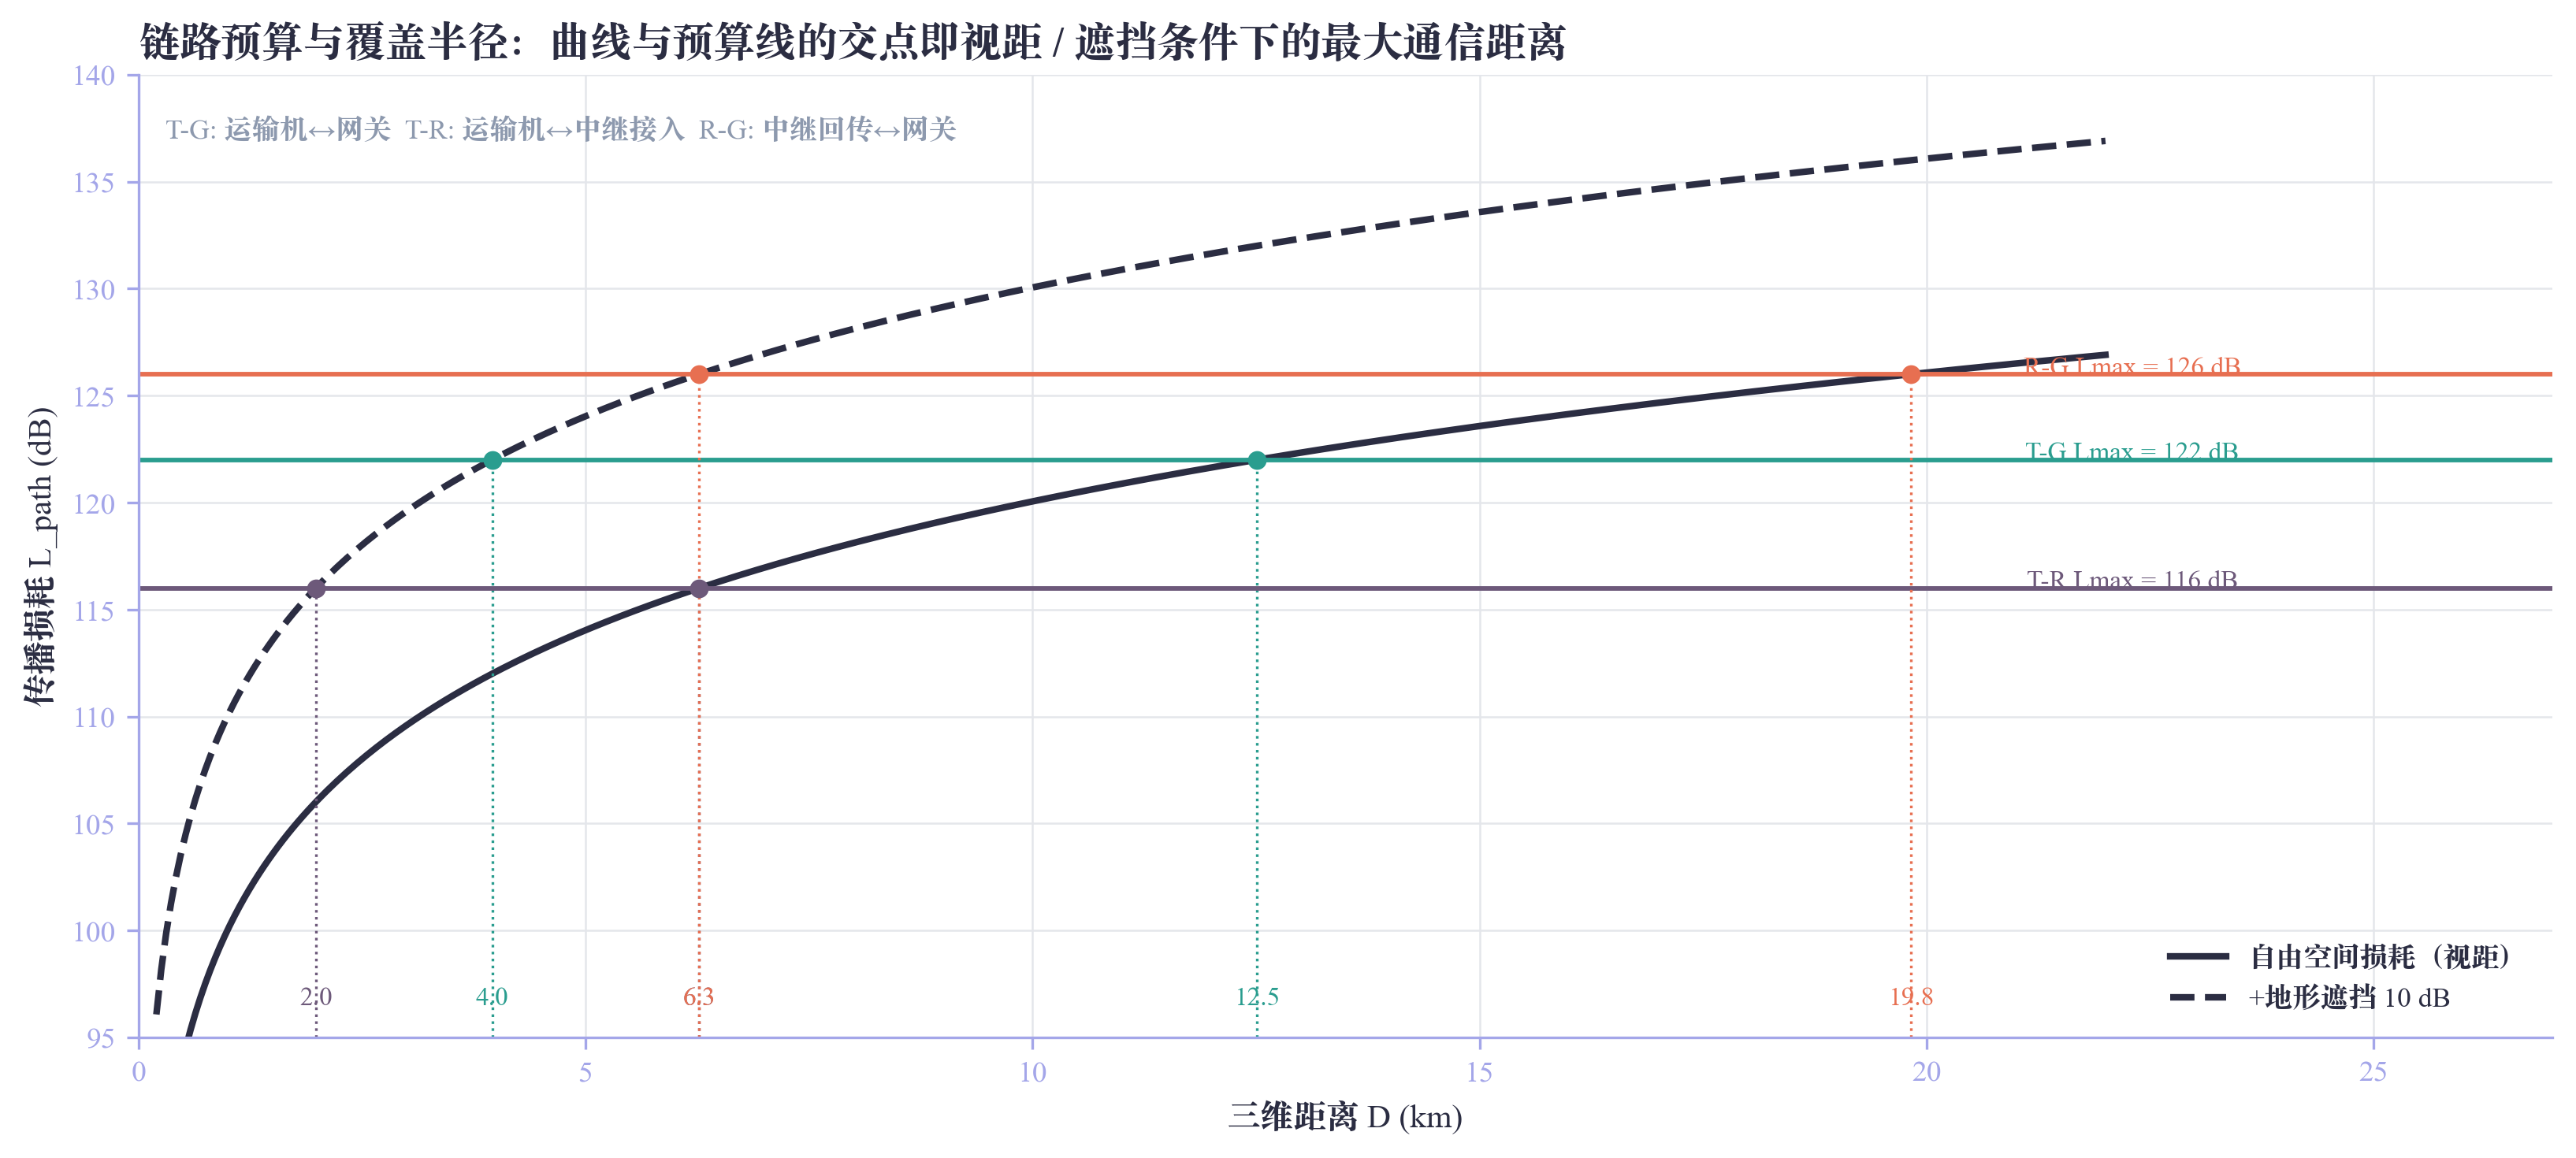
\includegraphics[width=\linewidth]{figures/Q3/图01_链路预算与覆盖半径.png}
\caption{不同通信链路的预算与等效覆盖半径}
\label{fig:q3-link-budget}
\end{figure}

\subsection{直连通性盲区分析（空间层 I）}

将 O01、15 个服务区及其间的有向航段纳入通信检查，共有 $240$ 条候选航段。沿运输机爬升、巡航和下降轨迹采样，并以 DEM 剖面判断视线遮挡；直连仅在路径损耗不超过运输机--G01 链路预算时判为可用。共检查 $56{,}648$ 个航迹采样点，其中 $27{,}950$ 个不能直连，占 $49.3\%$；15 个服务区中有 12 个无法由 G01 直接覆盖。研究区网格评估中，运输机离地高度为 $30\,\mathrm{m}$ 和 $300\,\mathrm{m}$ 时的直连覆盖率分别为 $20.5\%$ 和 $40.5\%$，表明仅提高飞行高度仍不足以消除山区通信盲区。

图~\ref{fig:q3-direct-shadow}展示航段采样点的直连状态。典型航段 O01--S002 的剖面中，直连通信中断占航段时间的 $45.3\%$；其地形与链路损耗变化见图~\ref{fig:q3-profile}。

\begin{figure}[H]
\centering
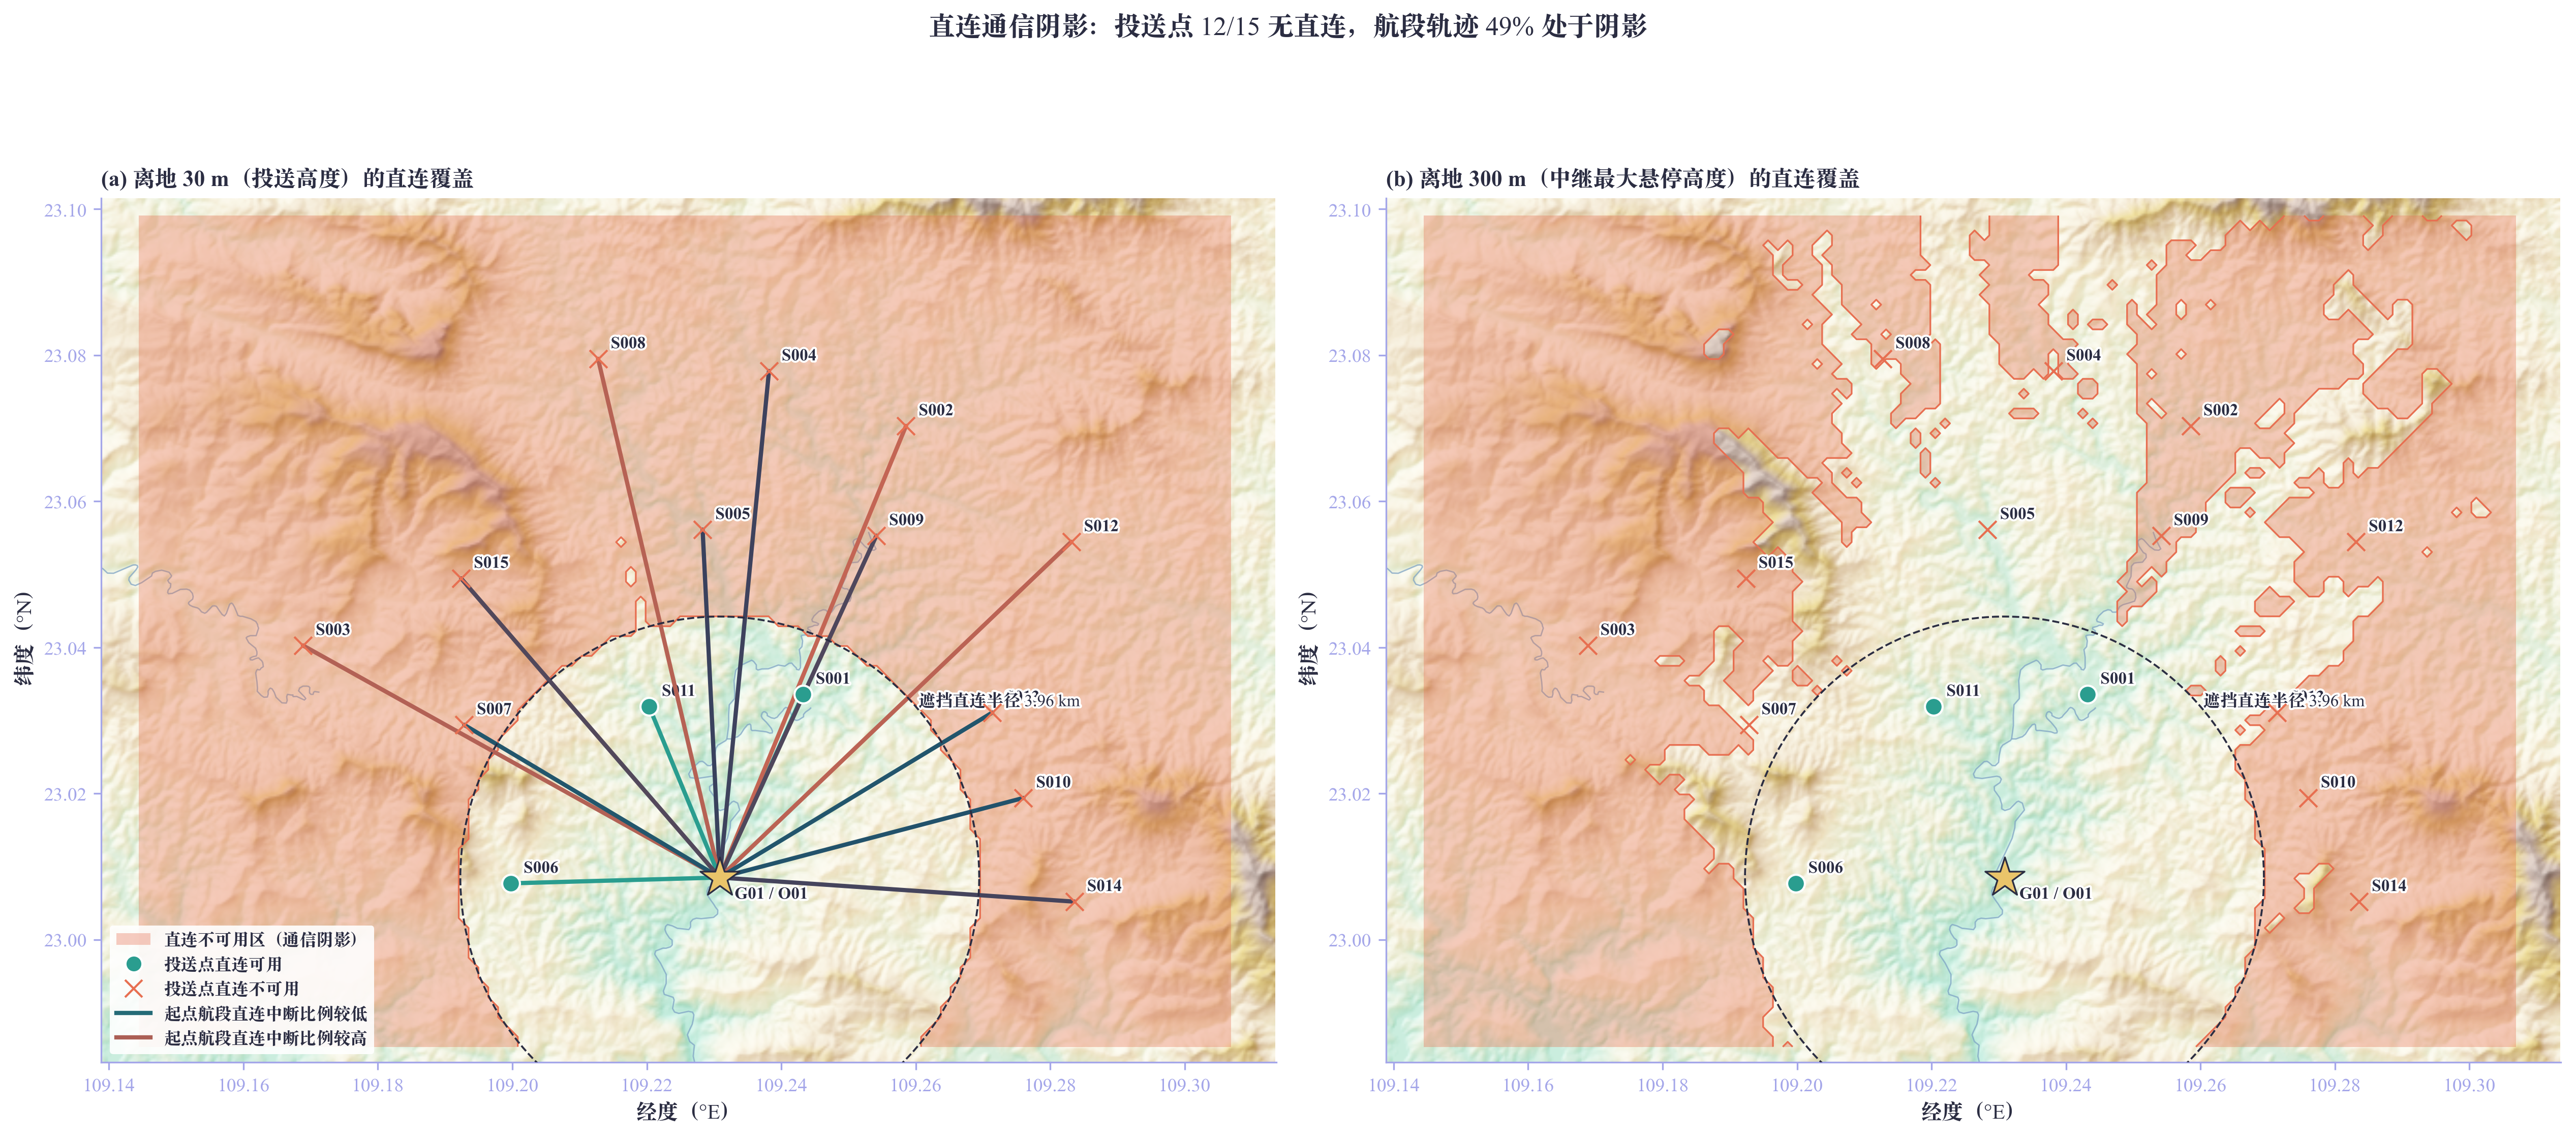
\includegraphics[width=\linewidth]{figures/Q3/图02_直连通信阴影图.png}
\caption{运输航段的直连通信状态与地形阴影分布}
\label{fig:q3-direct-shadow}
\end{figure}

\subsection{中继站选址（空间层 II）}

在研究区内按 $400\,\mathrm{m}$ 网格生成候选悬停点，并向 DEM 边界外扩 $1.5\,\mathrm{km}$；候选点均取离地 $300\,\mathrm{m}$。候选点须先满足中继机--G01 回传链路预算，生成的 $1{,}073$ 个候选点中有 $656$ 个通过该筛选。对运输轨迹直连盲区按 $150\,\mathrm{m}\times150\,\mathrm{m}\times40\,\mathrm{m}$ 空间体素归并，得到 $2{,}048$ 个代表点；12 个直连不可用的服务区交接点另赋较高权重。随后采用贪心最大覆盖，逐次选择新增覆盖权重最大的站点。

算法选出三个固定悬停位置 RS1--RS3，累计覆盖全部代表盲区点，并使 15 个服务区交接点均有中继覆盖。表~\ref{tab:q3-sites}列出其坐标、回传链路与累计覆盖率。这里的“三个站点”是空间位置数；时间层由两架中继无人机 R01、R02 在不同任务时段轮换服务。

\begin{table}[!htbp]
\centering
\caption{中继站位置与盲区覆盖结果}
\label{tab:q3-sites}
\scriptsize
\setlength{\tabcolsep}{3pt}
\begin{tabularx}{\textwidth}{@{}lccccccX@{}}
\toprule
站点 & 经度 & 纬度 & 地面海拔（m） & 悬停海拔（m） & 距 G01（km） & 回传损耗（dB） & 累计覆盖率 \\
\midrule
RS1 & 109.205 & 23.046 & 459 & 759 & 4.952 & 113.949 & 71.7\% \\
RS2 & 109.283 & 23.017 & 446 & 746 & 5.459 & 124.796 & 99.9\% \\
RS3 & 109.189 & 23.068 & 719 & 1019 & 7.847 & 117.948 & 100.0\% \\
\bottomrule
\end{tabularx}
\end{table}

RS2 的回传损耗最接近 $126\,\mathrm{dB}$ 预算，但仍通过筛选。图~\ref{fig:q3-stations}展示候选盲区及站点覆盖；典型航段的地形剖面和链路损耗对比如图~\ref{fig:q3-profile}所示。

\begin{figure}[H]
\centering
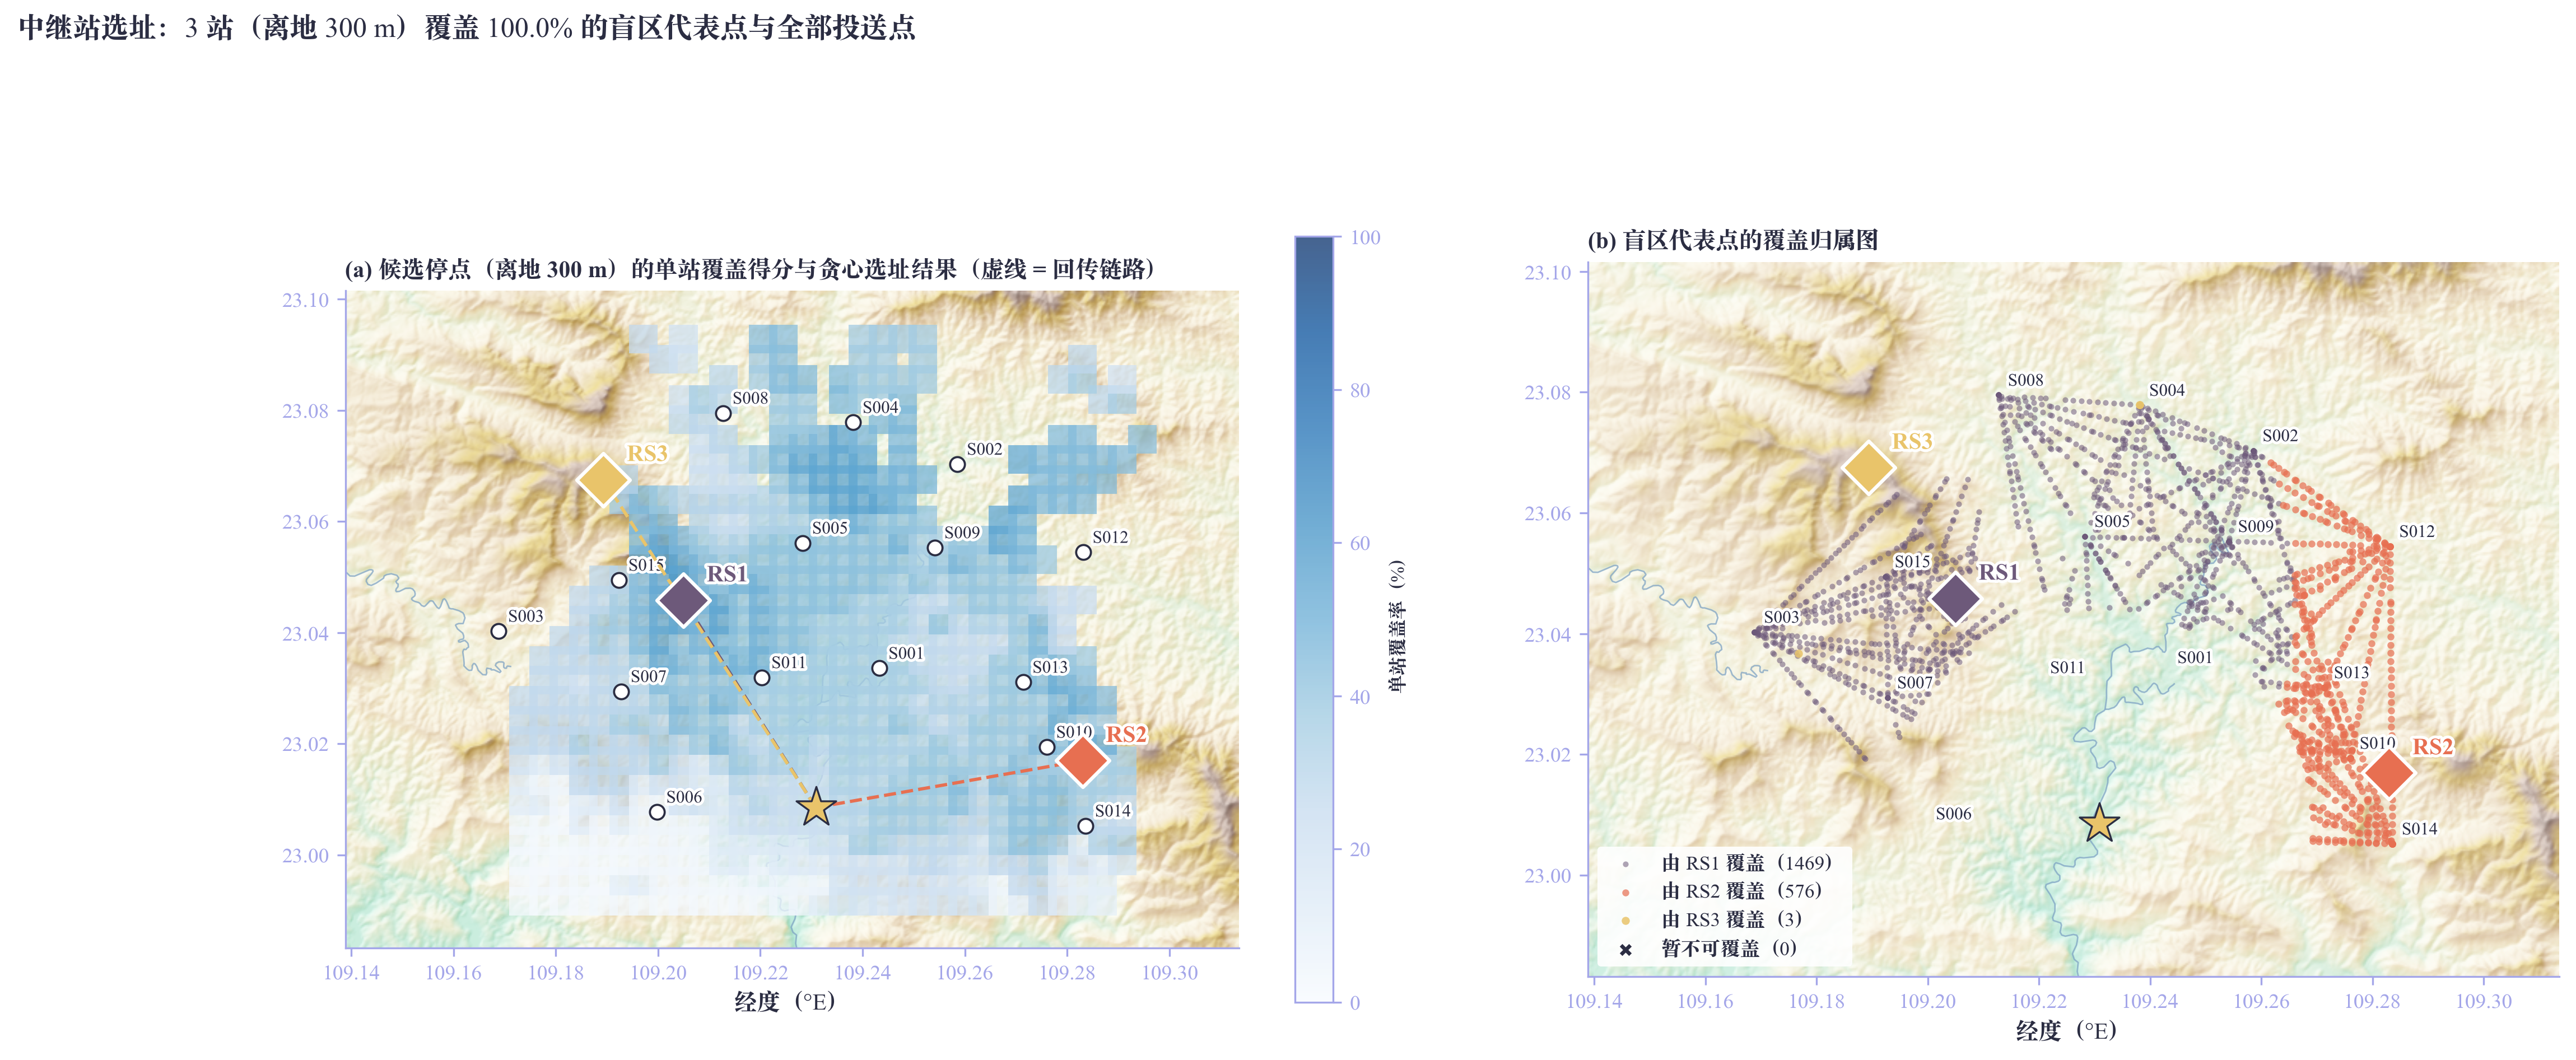
\includegraphics[width=\linewidth]{figures/Q3/图03_中继站选址.png}
\caption{中继站选址及对直连盲区的累计覆盖}
\label{fig:q3-stations}
\end{figure}

\begin{figure}[H]
\centering
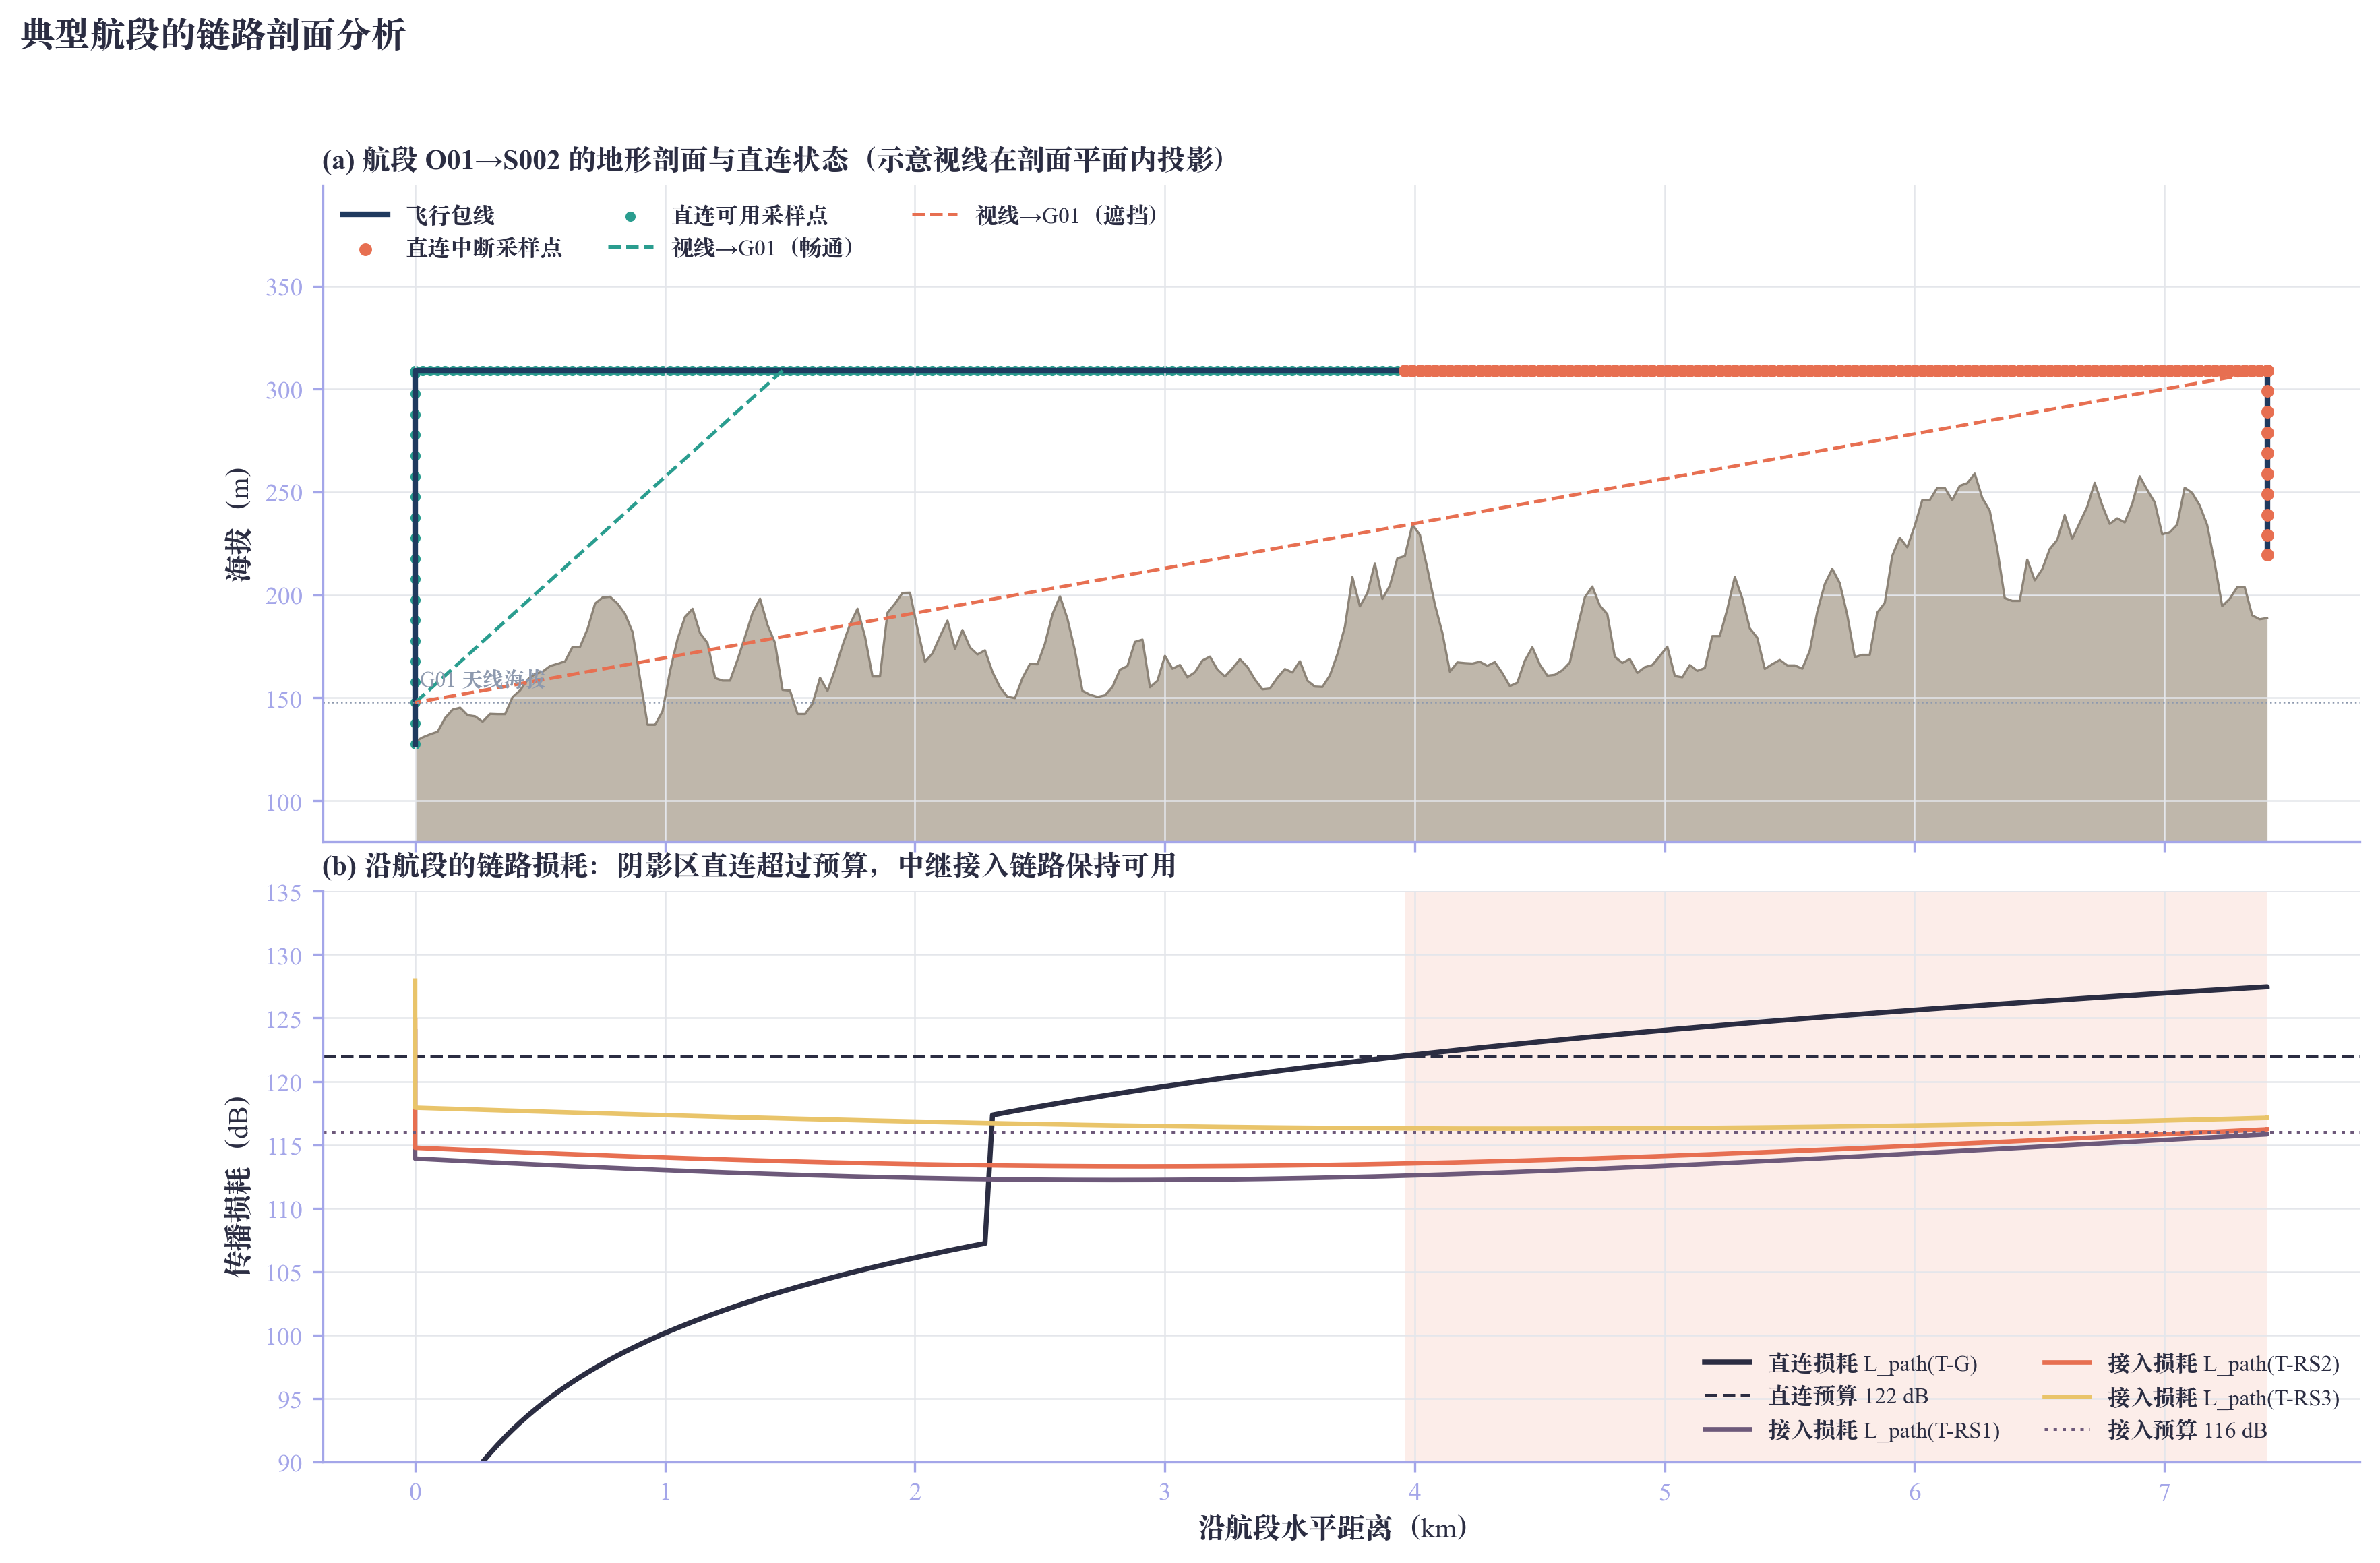
\includegraphics[width=\linewidth]{figures/Q3/图04_典型航段链路剖面.png}
\caption{典型运输航段的地形剖面与链路损耗}
\label{fig:q3-profile}
\end{figure}

\subsection{时间层：中继需求区间与联合列表调度}

对 $240$ 条航段及 A、B、C 三类运输机生成 $1{,}296$ 组航段需求区间，并将交接期间的通信需求一并纳入排程。直连中断时，解码器为相应区间指定一个站点，使运输机--中继机接入链路和中继机--G01 回传链路同时可用；同一需求区间由单个站点连续保障。记 $a_p(t)$ 为运输机 $p$ 在时刻 $t$ 的直连状态，$z_{ps}(t)$ 为其由站点 $s$ 中继的状态，则连续通信约束写为
\begin{equation}
\begin{aligned}
a_p(t)+\sum_s z_{ps}(t)&\ge 1,\\
\sum_s z_{ps}(t)&\le 1,\\
z_{ps}(t)&\le 1-a_p(t),\\
z_{ps}(t)&\le \mathbf{1}\!\left(L_{p,s}^{\mathrm{T-R}}(t)\le116\,\mathrm{dB}\right),\\
z_{ps}(t)&\le \mathbf{1}\!\left(L_s^{\mathrm{R-G}}(t)\le126\,\mathrm{dB}\right),\\
z_{ps}(t)&\le y_s(t).
\end{aligned}
\label{eq:q3-communication}
\end{equation}
其中 $y_s(t)$ 表示站点 $s$ 在时刻 $t$ 在线。若需求到达时中继机尚未到位或其能源组件仍在充电，列表解码器会推迟运输架次，最多重试 6 次；仍不能满足时，该候选方案判为不可行。

中继机从 O01 出发，经固定准备、爬升、巡航和建链后在站悬停。站上悬停与通信功率合计为 $1.10\,\mathrm{kW}$；能源组件总容量为 $3.2\,\mathrm{kWh}$，保留 $20\%$ 返航电量后，单次任务能耗上限为 $2.56\,\mathrm{kWh}$。若中继会话在 $t_{\mathrm{linked}}$ 时建链完成、于 $t_{\mathrm{leave}}$ 离站，则
\begin{equation}
E_s^{\mathrm{out}}+E_s^{\mathrm{back}}
+1.10\,\frac{30+t_{\mathrm{leave}}-t_{\mathrm{linked}}}{3600}
\le 2.56\,\mathrm{kWh}.
\label{eq:q3-relay-energy}
\end{equation}
两架中继机、六组能源组件按 $300\,\mathrm{s}$ 机体周转和两阶段充电规则共同排程；组件充满时间为 $1{,}800\,\mathrm{s}$。各站点对应的飞行耗时与单组件最长在站能力见表~\ref{tab:q3-relay-flight}。

\begin{table}[!htbp]
\centering
\caption{中继机往返飞行与在站服务能力}
\label{tab:q3-relay-flight}
\scriptsize
\setlength{\tabcolsep}{4pt}
\begin{tabularx}{\textwidth}{@{}lcccccX@{}}
\toprule
站点 & O01 至站点（km） & 去程（s） & 返程（s） & 往返飞行能耗（kWh） & 最早建链时刻（s） & 单组件最长在站时间（h） \\
\midrule
RS1 & 4.91 & 485 & 538 & 0.265 & 695 & 2.08 \\
RS2 & 5.43 & 516 & 568 & 0.286 & 726 & 2.06 \\
RS3 & 7.80 & 743 & 817 & 0.411 & 953 & 1.94 \\
\bottomrule
\end{tabularx}
\end{table}

联合目标沿用式~\eqref{eq:q2-timeliness} 的及时性指标，并将完工时间、总能耗和架次数扩展为运输与中继的联合量：
\begin{equation}
f_M=\frac{\max\{t_T^{\mathrm{end}},t_R^{\mathrm{end}}\}}{3600},\qquad
f_E=\sum_{p\in P}E_p+\sum_{q\in Q}E_q,\qquad
f_N=|P|+|Q|.
\label{eq:q3-joint-metrics}
\end{equation}
搜索时采用与问题二一致的归一化加权和，推荐权重为 $(w_T,w_M,w_E,w_N)=(3,1.5,1,0.5)$；硬时限迟到与通信中断分别按每小时 $100$、每次 $5$ 的规则惩罚。求解仍采用 ALNS：以货箱移除和插入改变运输组批及访问顺序，由联合列表解码器排定运输无人机、电池、中继机和能源组件；主搜索运行 $8{,}000$ 次迭代，并对及时性、完工时间、能耗和架次数偏好分别运行 $2{,}500$ 次。通信不可行候选不进入可行解记录。图~\ref{fig:q3-alns}给出主搜索的目标值及破坏算子权重变化。

\begin{figure}[H]
\centering
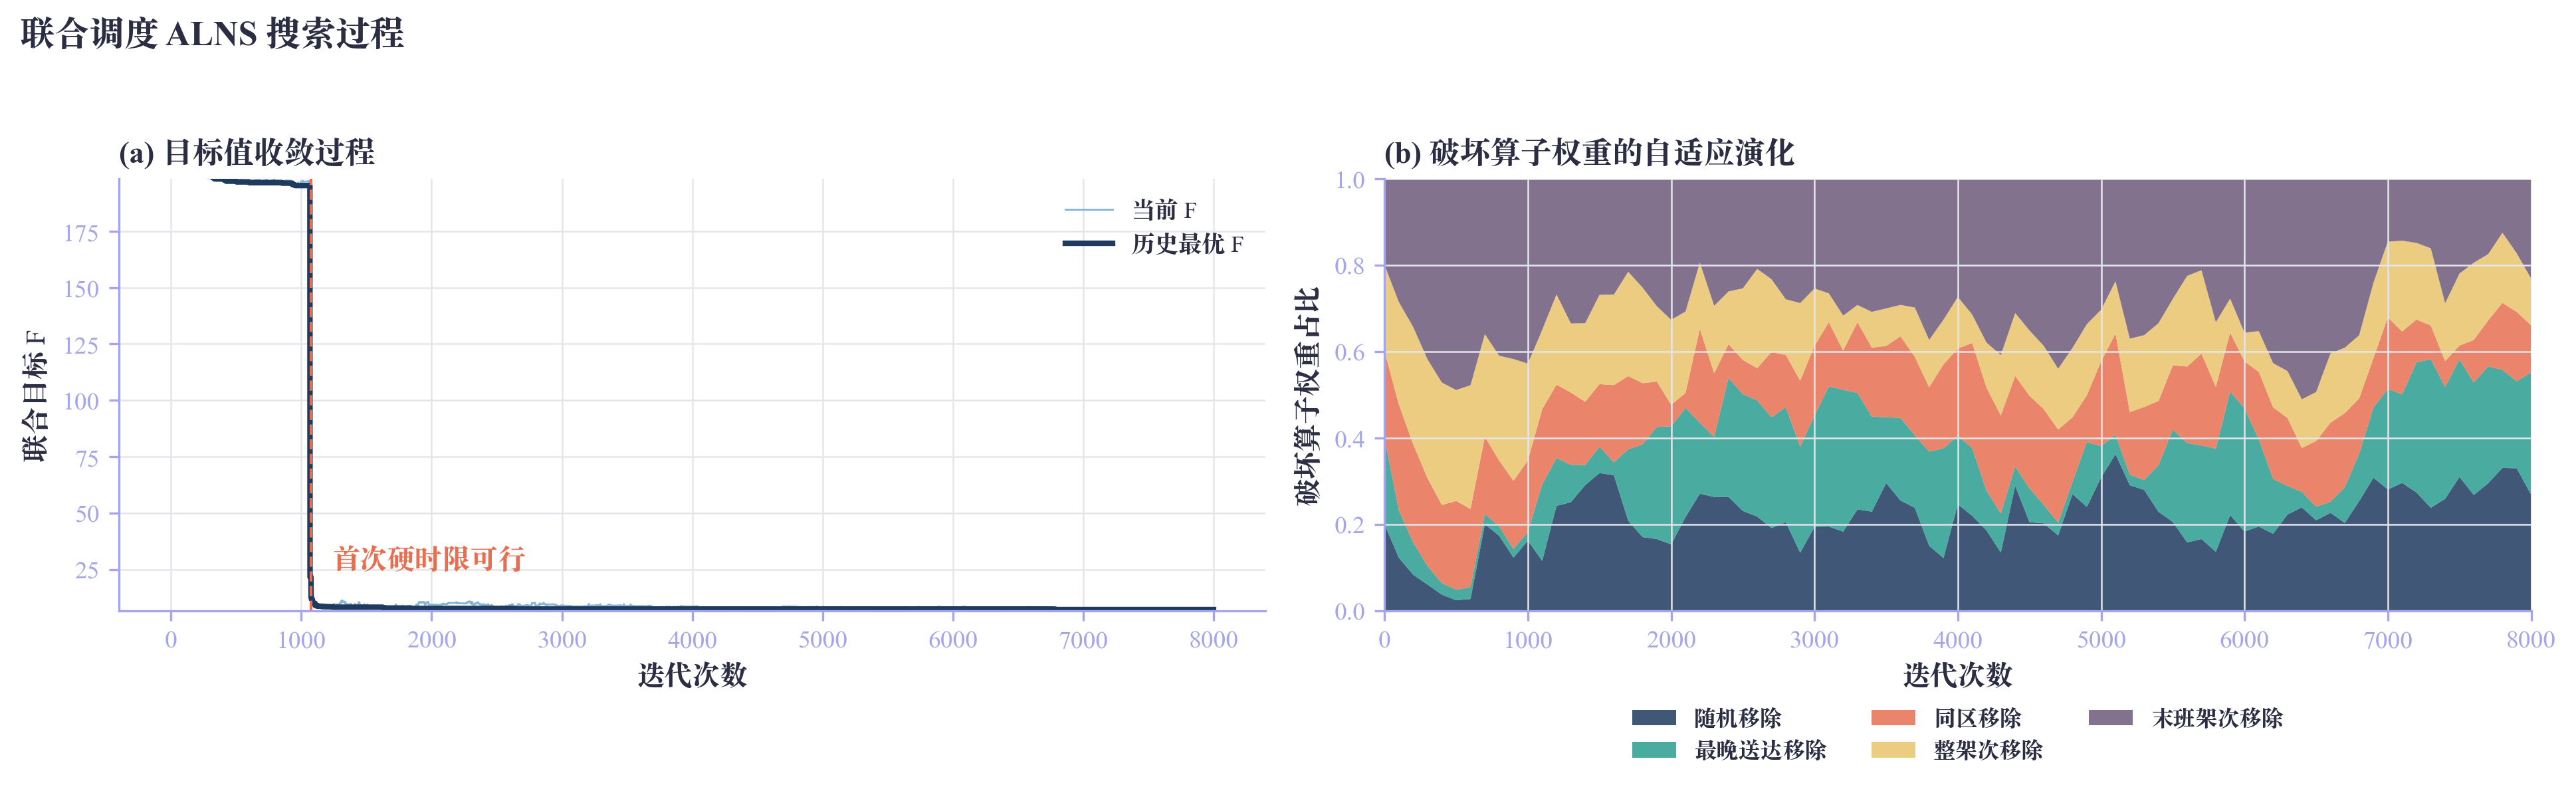
\includegraphics[width=\linewidth]{figures/Q3/图05_ALNS搜索过程.png}
\caption{联合调度 ALNS 的目标收敛与破坏算子权重演化}
\label{fig:q3-alns}
\end{figure}

\subsection{推荐联合方案与结果分析}

从主搜索和四种偏好搜索的可行候选中，按推荐权重重新评价并选取 $F$ 最小者。推荐解的 $F=6.957$，$f_T=0.134$，联合完工时间为 $2.819\,\mathrm{h}$，其中运输任务完工于 $2.786\,\mathrm{h}$。方案配送 80 箱，使用 A、B、C 型运输机分别执行 11、7、6 个架次；另由两架中继机执行 4 个中继架次。运输能耗为 $76.404\,\mathrm{kWh}$，中继能耗为 $4.967\,\mathrm{kWh}$，总能耗为 $81.371\,\mathrm{kWh}$。优先加权平均迟到为 $119.303\,\mathrm{s}$，加权平均送达时刻为 $3{,}617.919\,\mathrm{s}$；11 箱晚于期望送达时刻，但 31 箱硬时限全部满足，最小提前量为 $0.8\,\mathrm{min}$。

\begin{table}[!htbp]
\centering
\caption{推荐联合方案的主要指标}
\label{tab:q3-recommended}
\scriptsize
\setlength{\tabcolsep}{5pt}
\begin{tabularx}{\textwidth}{@{}XcXc@{}}
\toprule
指标 & 结果 & 指标 & 结果 \\
\midrule
联合目标 $F$ & 6.957 & 及时性 $f_T$ & 0.134 \\
联合完工时间 & $2.819\,\mathrm{h}$ & 运输完工时间 & $2.786\,\mathrm{h}$ \\
运输能耗 & $76.404\,\mathrm{kWh}$ & 中继能耗 & $4.967\,\mathrm{kWh}$ \\
运输架次 & 24 & 中继架次 & 4 \\
硬时限违约箱数 & 0 & 最小硬时限提前量 & $0.8\,\mathrm{min}$ \\
\bottomrule
\end{tabularx}
\end{table}

四次中继会话依次为 R01 服务 RS1（$2.39\,\mathrm{kWh}$）、R02 服务 RS2（$1.17\,\mathrm{kWh}$）、R02 服务 RS3（$0.94\,\mathrm{kWh}$）和 R02 服务 RS2（$0.47\,\mathrm{kWh}$），均未超过式~\eqref{eq:q3-relay-energy} 的单次能耗上限。空间联合航线见图~\ref{fig:q3-routes}；图~\ref{fig:q3-gantt}展示运输与中继任务时序，图~\ref{fig:q3-communication}汇总通信状态、站点在线时段及中继能耗构成。

\begin{figure}[H]
\centering
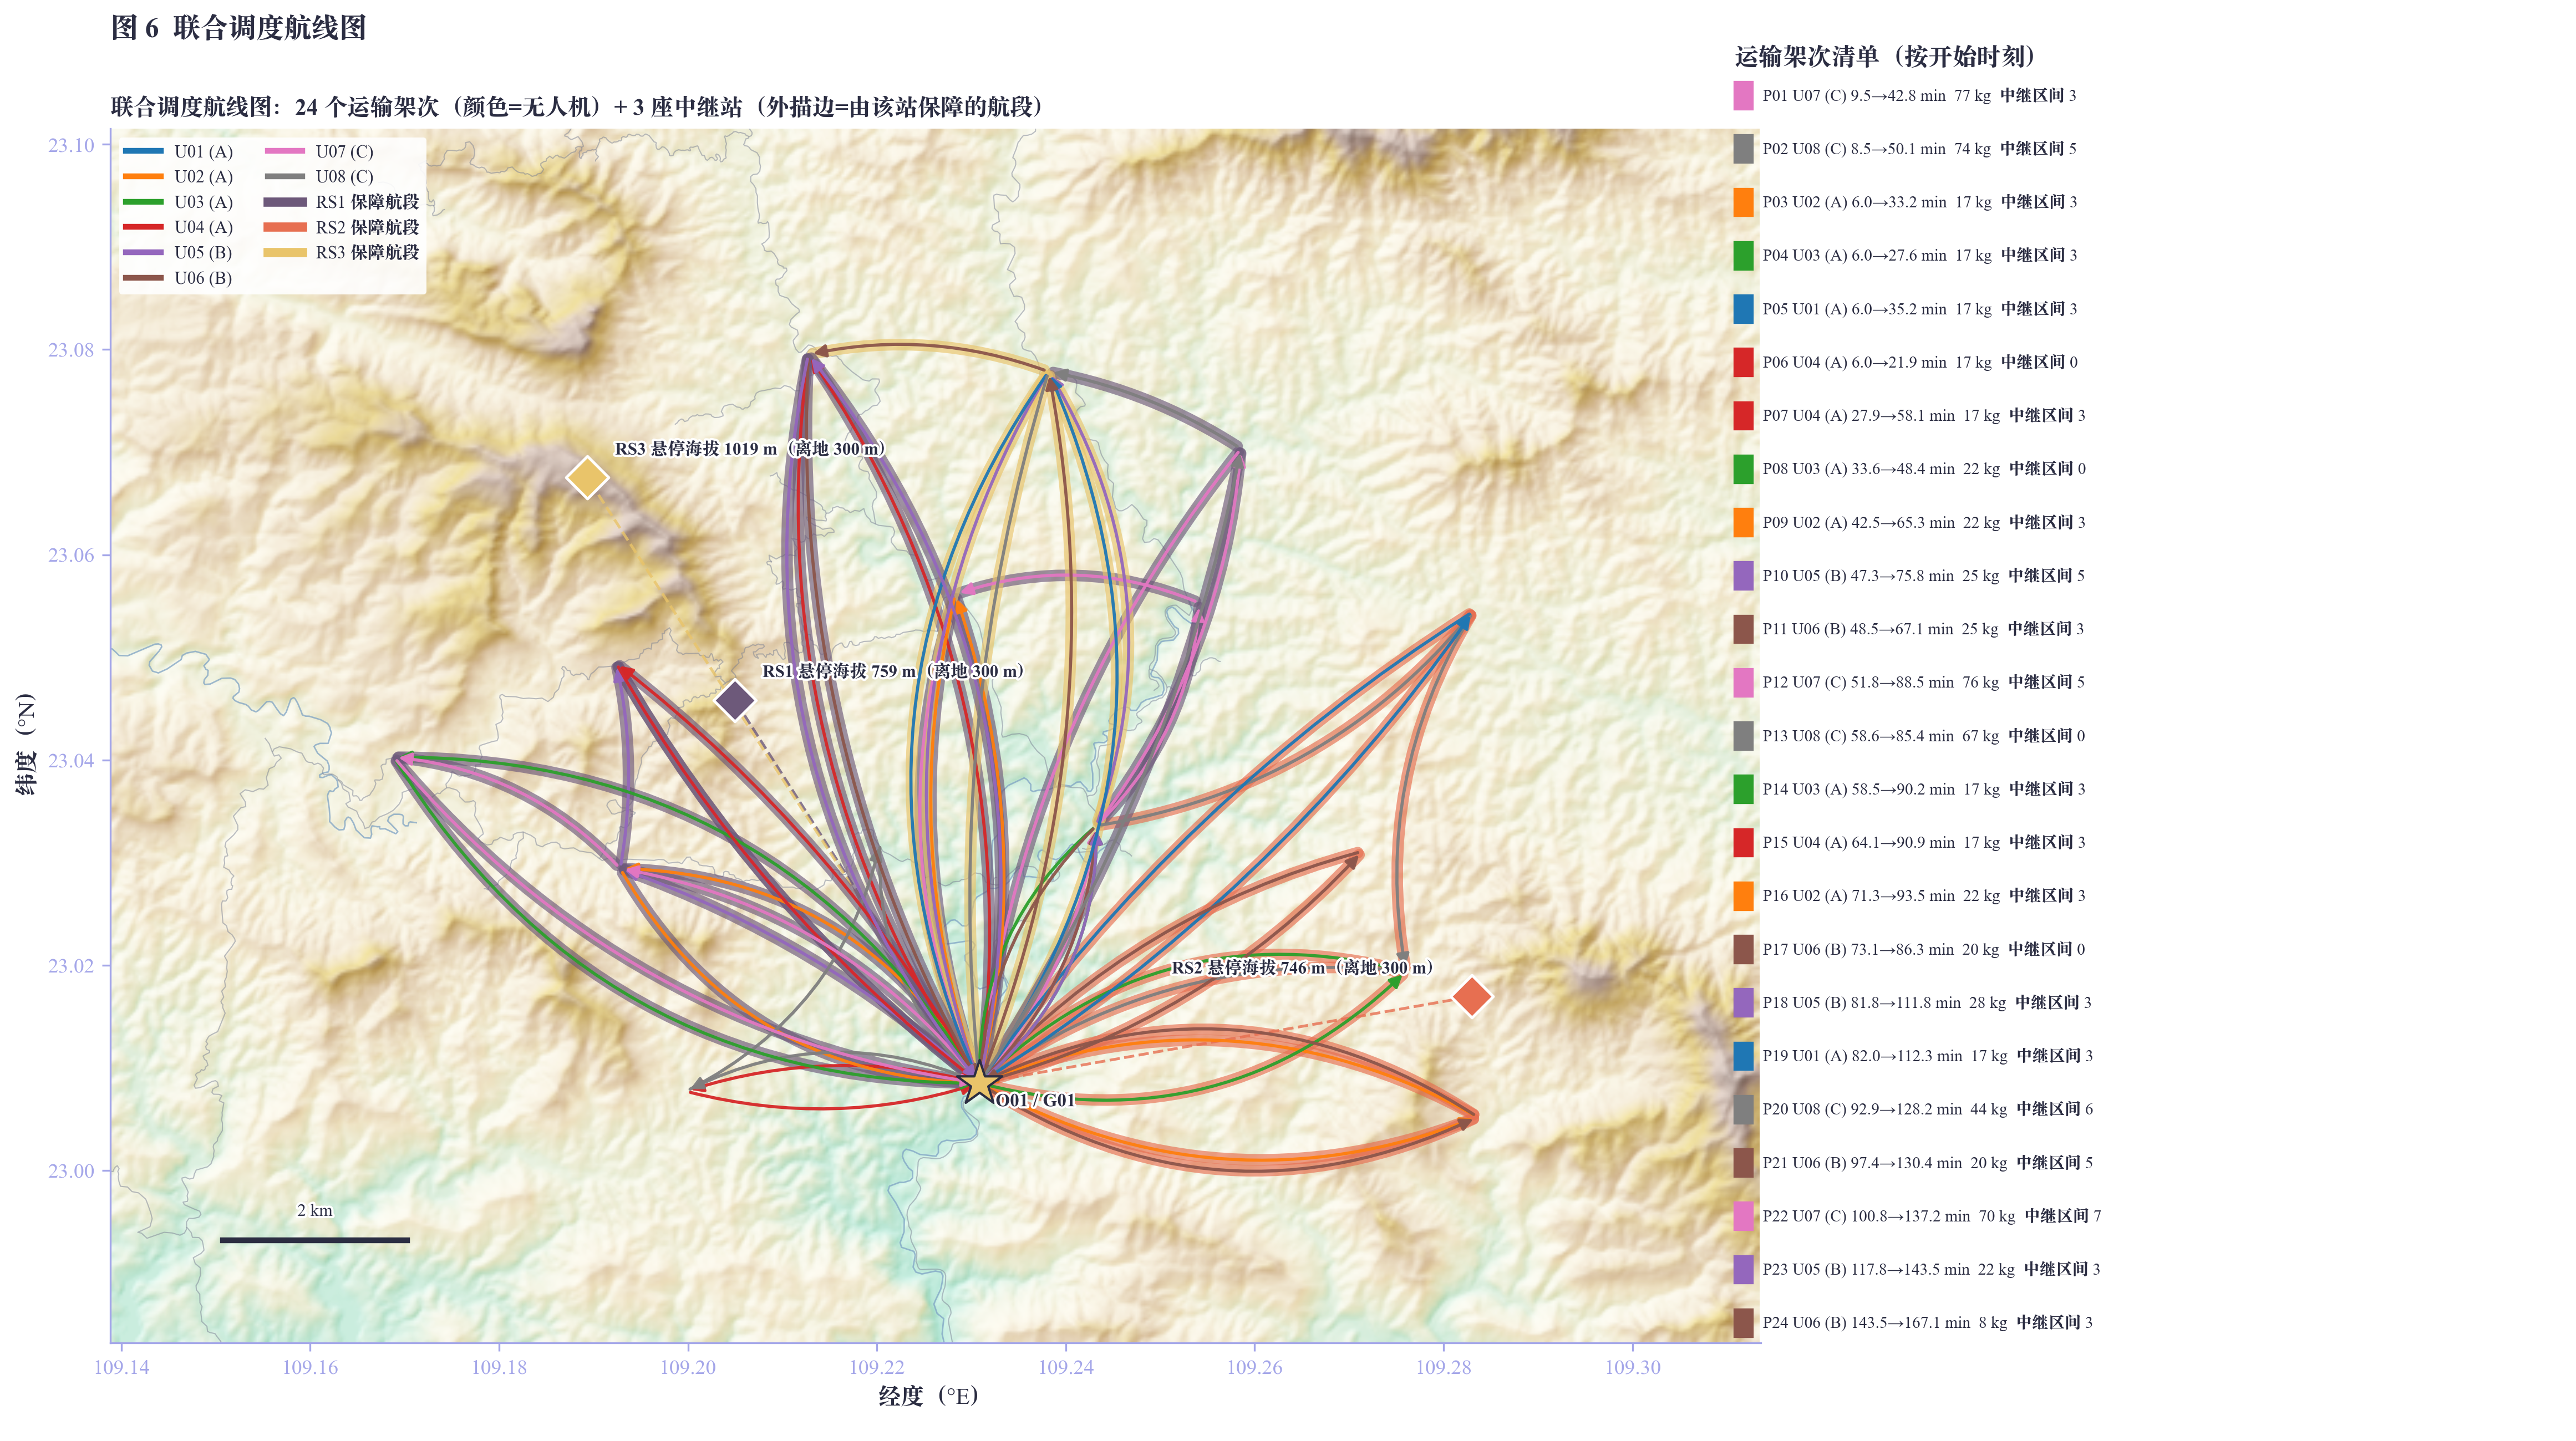
\includegraphics[width=\linewidth]{figures/Q3/图06_联合调度航线图.png}
\caption{推荐联合方案的运输航线、中继站点与保障航线}
\label{fig:q3-routes}
\end{figure}

\begin{figure}[H]
\centering
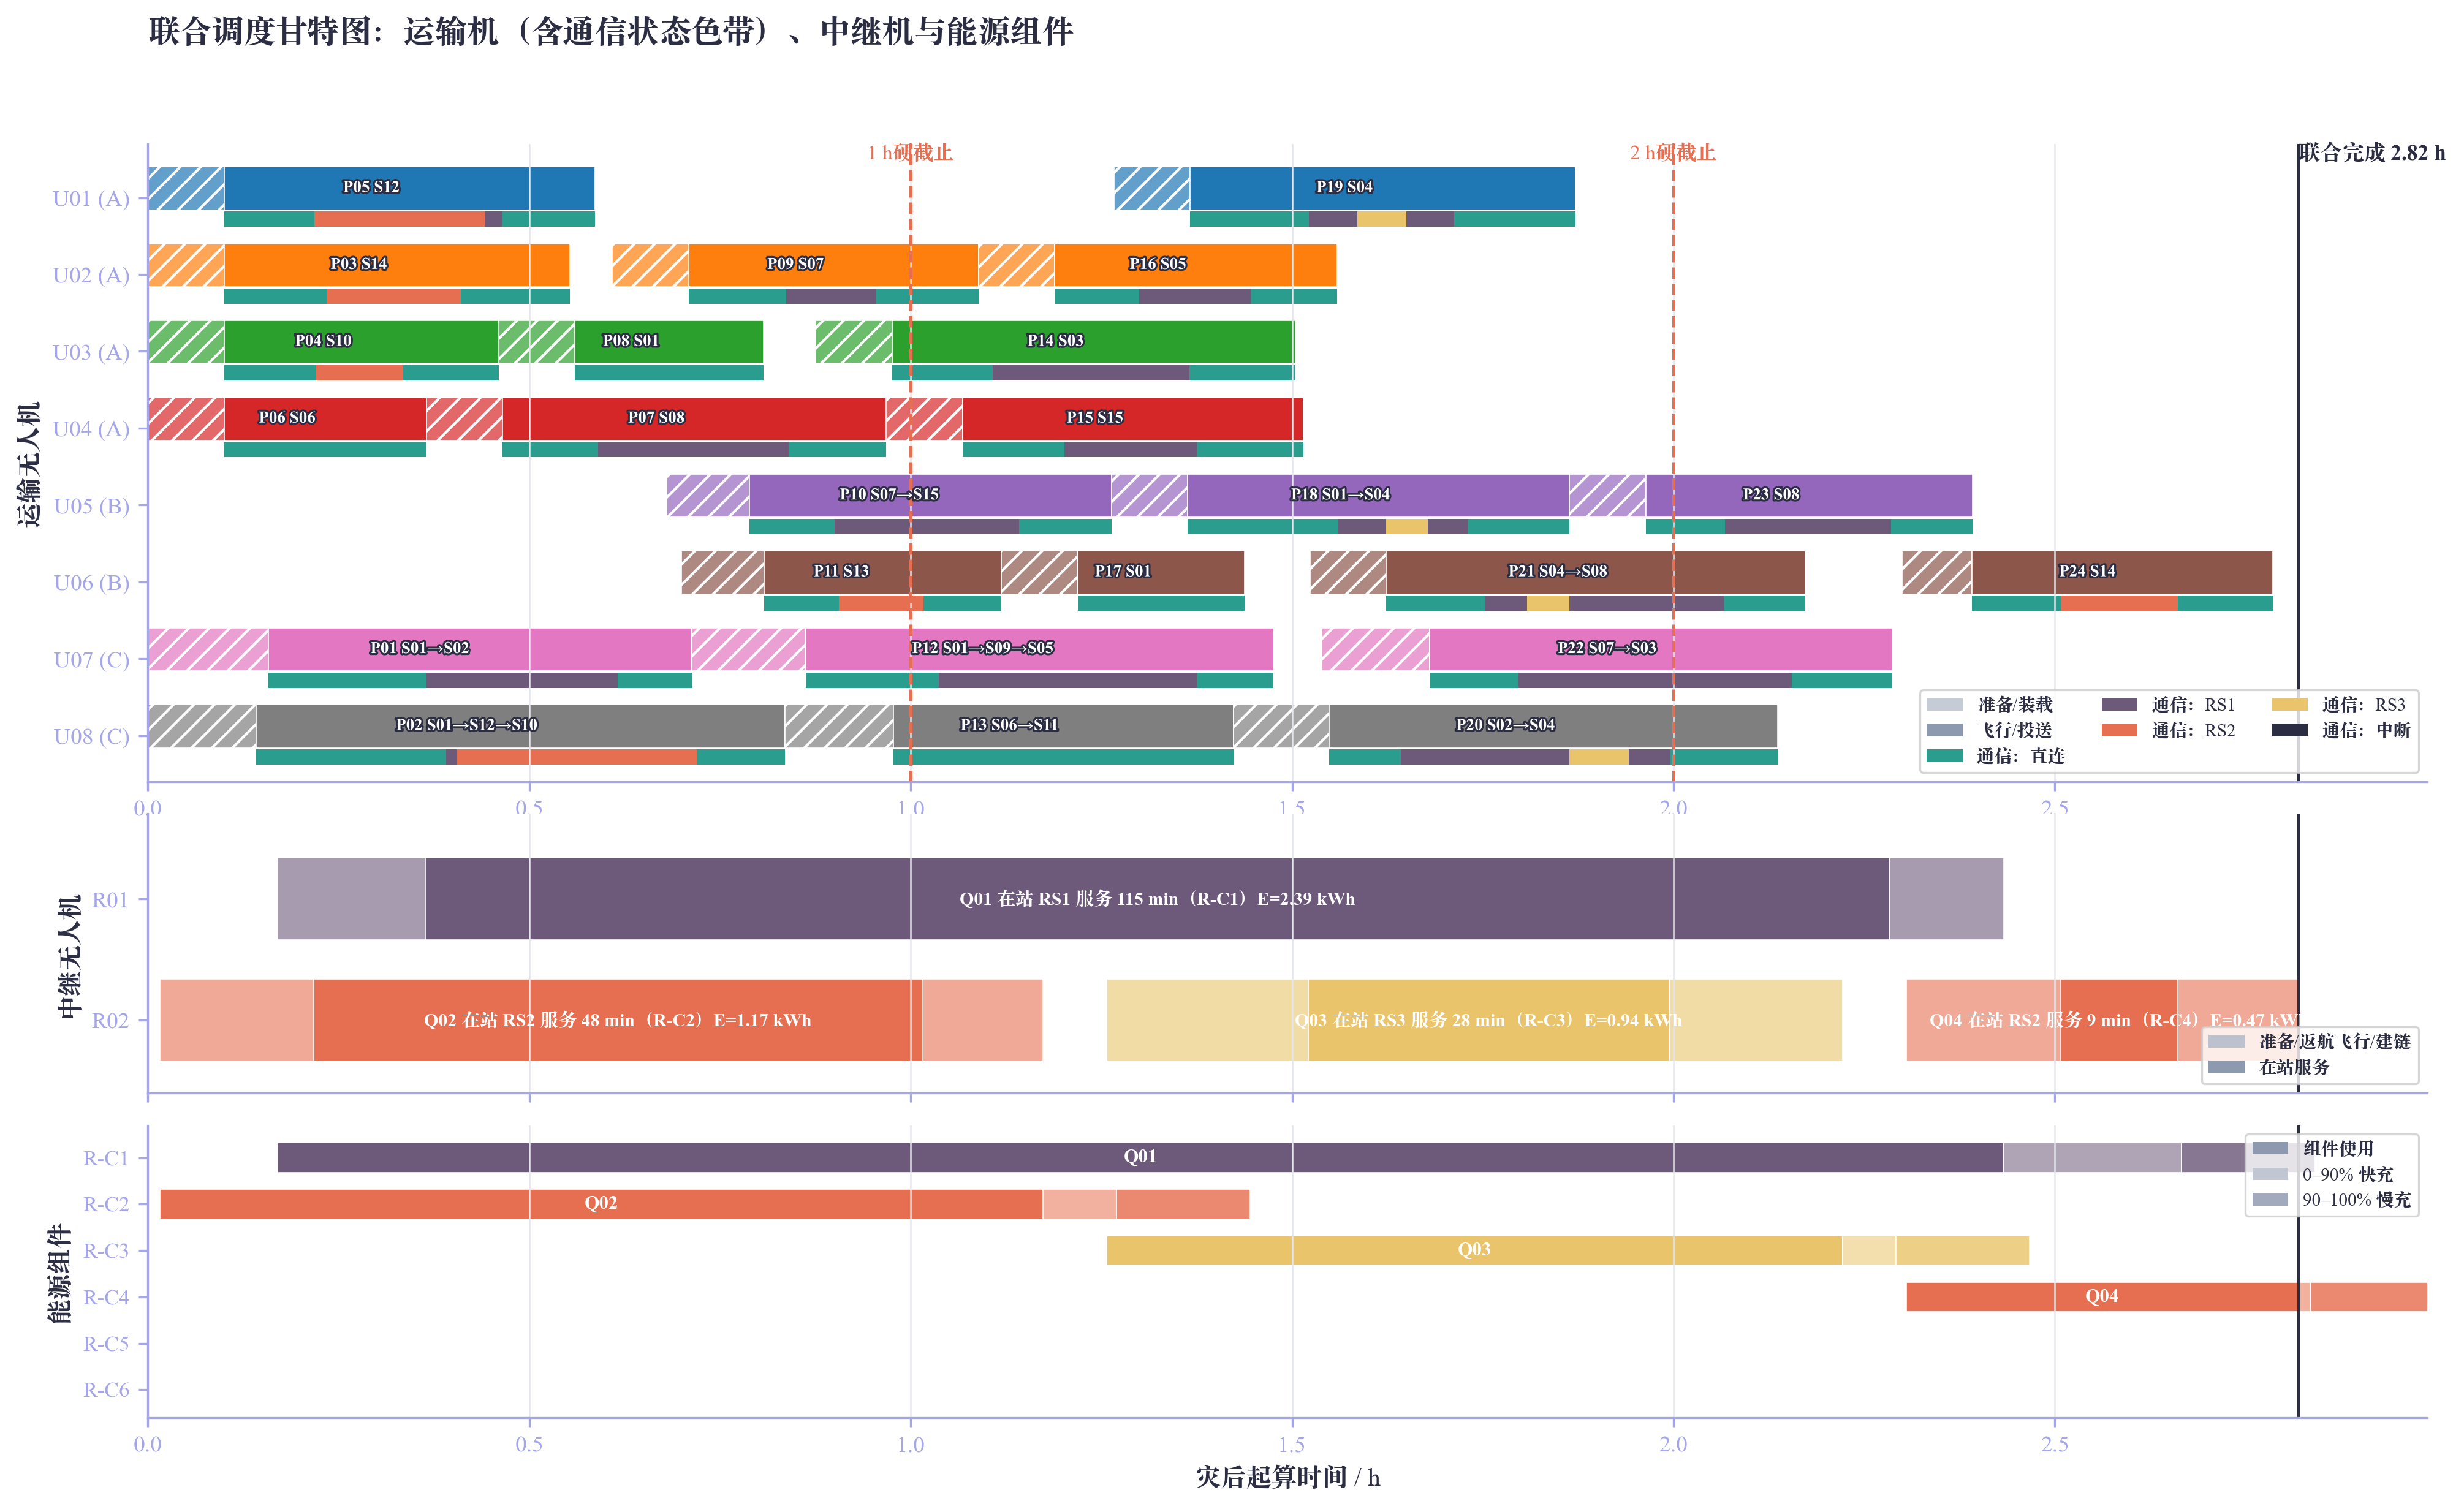
\includegraphics[width=\linewidth]{figures/Q3/图07_联合调度甘特图.png}
\caption{运输无人机、中继无人机与能源组件的联合调度时序}
\label{fig:q3-gantt}
\end{figure}

\begin{figure}[H]
\centering
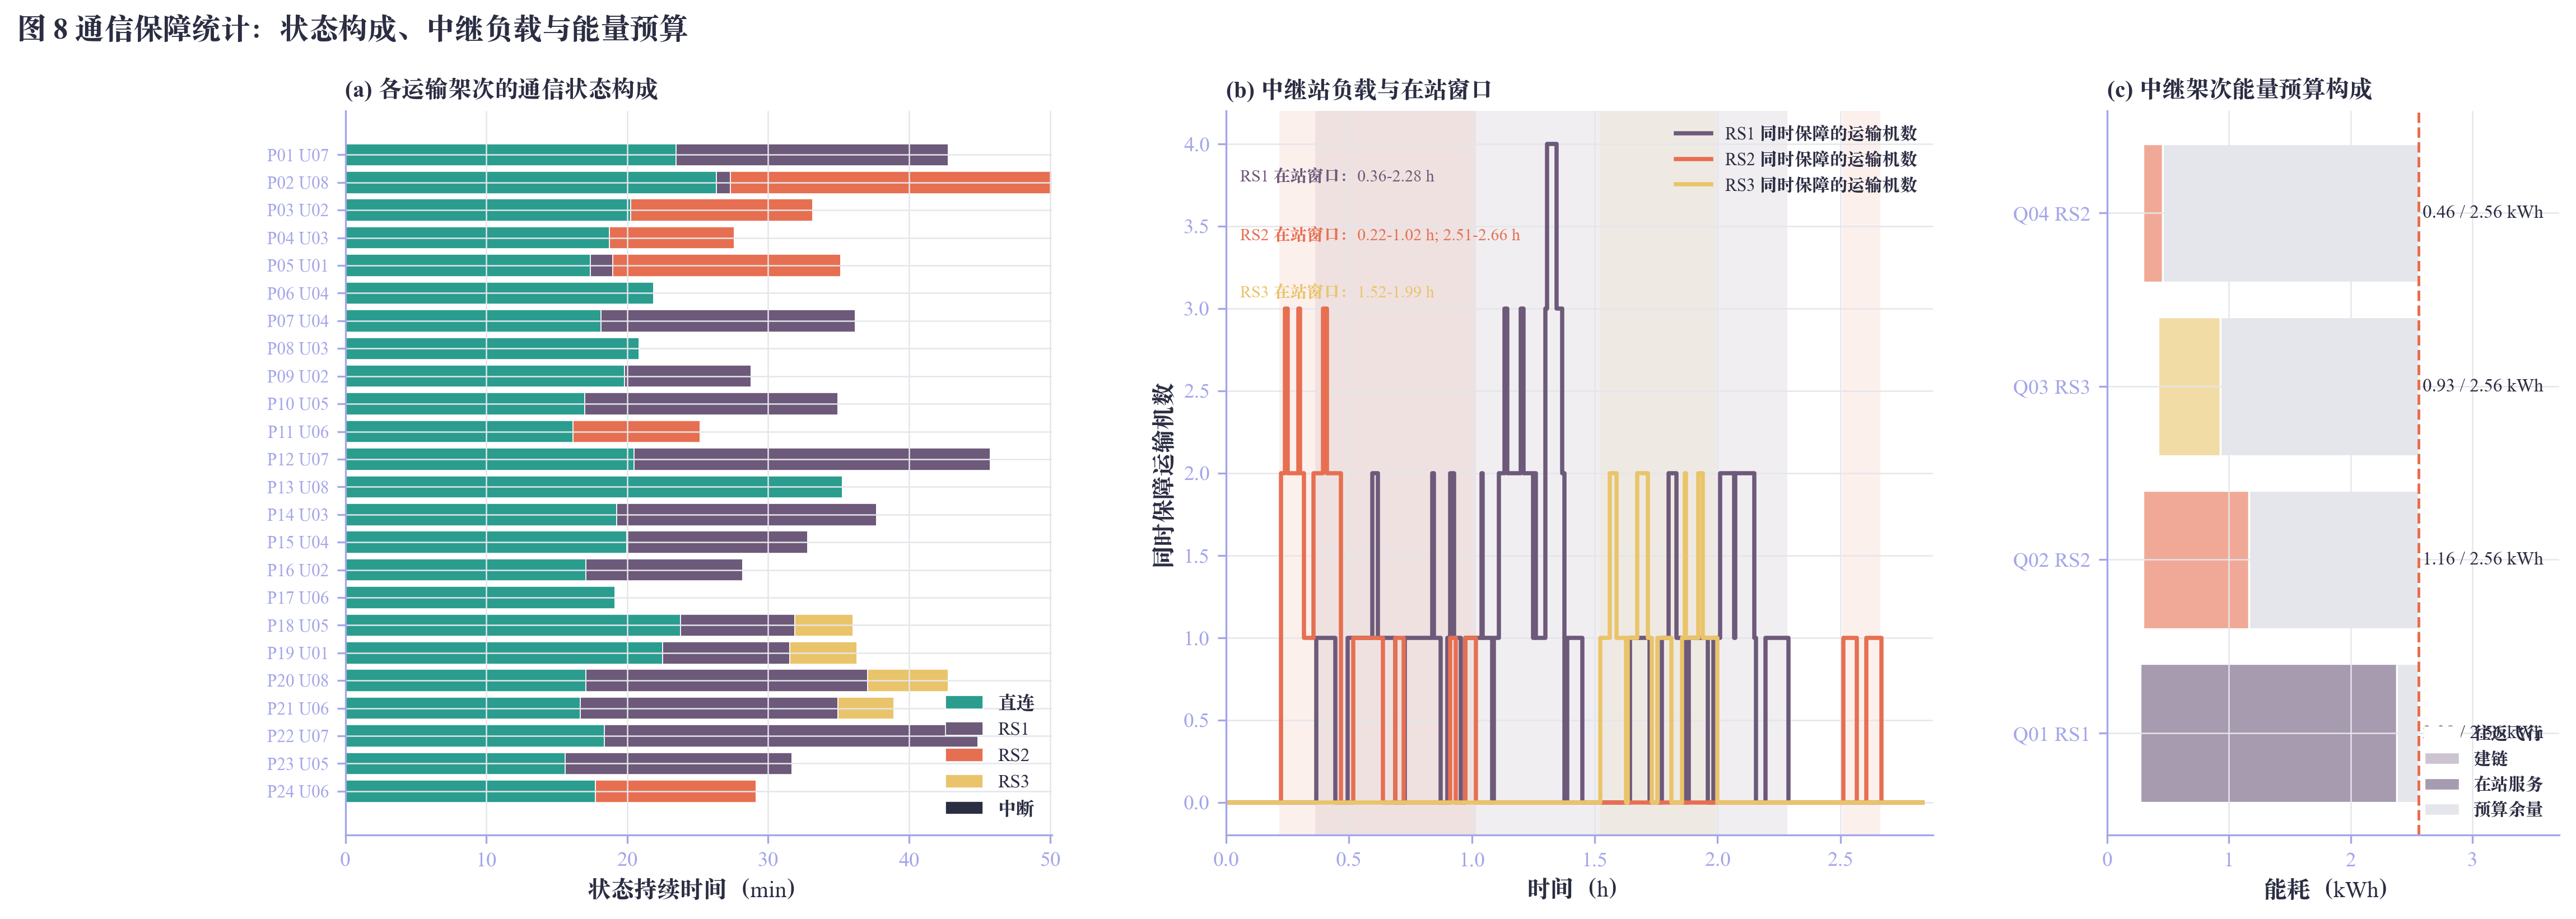
\includegraphics[width=\linewidth]{figures/Q3/图08_通信保障统计.png}
\caption{运输任务通信状态、中继站在线区间及能耗统计}
\label{fig:q3-communication}
\end{figure}

\subsection{联合四指标权衡与通信代价}

表~\ref{tab:q3-tradeoff}比较不同偏好下的已搜索可行方案。及时性优先方案取得较小的 $f_T$；能耗优先方案将总能耗降至 $75.718\,\mathrm{kWh}$；架次优先方案以 22 个运输与中继总架次完成任务，但完工时间增至 $3.709\,\mathrm{h}$。搜索记录包含 $2{,}301$ 个不同可行解，其中 69 个为记录集内的四指标非支配解；这只是启发式搜索记录，不代表完整 Pareto 前沿。图~\ref{fig:q3-tradeoff}展示情景方案及记录解之间的指标权衡。

\begin{table}[!htbp]
\centering
\caption{不同偏好下的联合调度可行方案}
\label{tab:q3-tradeoff}
\scriptsize
\setlength{\tabcolsep}{4pt}
\begin{tabularx}{\textwidth}{@{}Xcccc@{}}
\toprule
情景 & $f_T\downarrow$ & 联合完工时间（h）$\downarrow$ & 总能耗（kWh）$\downarrow$ & 总架次$\downarrow$ \\
\midrule
推荐权重（3, 1.5, 1, 0.5） & 0.134 & 2.819 & 81.371 & 28 \\
及时性优先 & 0.131 & 2.819 & 81.767 & 28 \\
完工时间优先 & 0.232 & 2.750 & 88.799 & 28 \\
能耗优先 & 0.301 & 3.016 & 75.718 & 24 \\
架次优先 & 0.307 & 3.709 & 79.401 & 22 \\
\bottomrule
\end{tabularx}
\end{table}

对推荐解逐项复核的 12 项约束检查全部通过：80 箱均恰好配送一次，质量、体积和能量约束满足；运输机与电池无资源冲突，最低运输机返航荷电状态为 $20.1\%$；中继架次均满足回传预算，最大单次中继能耗为 $2.39\,\mathrm{kWh}$，最低中继返航荷电状态为 $25\%$。此外，以 $5\,\mathrm{s}$ 间隔对运输时段独立采样 $7{,}929$ 个通信状态点，未发现中断。该检验支持本方案在既定地形、链路预算及离散采样模型下的可行性，但不等价于对真实无线信道连续时间性能的实测验证。

与问题二的推荐方案相比，问题三候选方案的总架次由 22 增至 28，总能耗由 $71.839$ 增至 $81.371\,\mathrm{kWh}$，完工时间由 $1.977$ 增至 $2.819\,\mathrm{h}$。该对比反映了两个分别优化后方案的总体差异；由于问题三同时引入中继资源并重新优化运输计划，不能将差值解释为隔离通信因素后的因果增量。图~\ref{fig:q3-soc-delivery}联合展示推荐方案的荷电状态与逐箱送达时刻。

\begin{figure}[H]
\centering
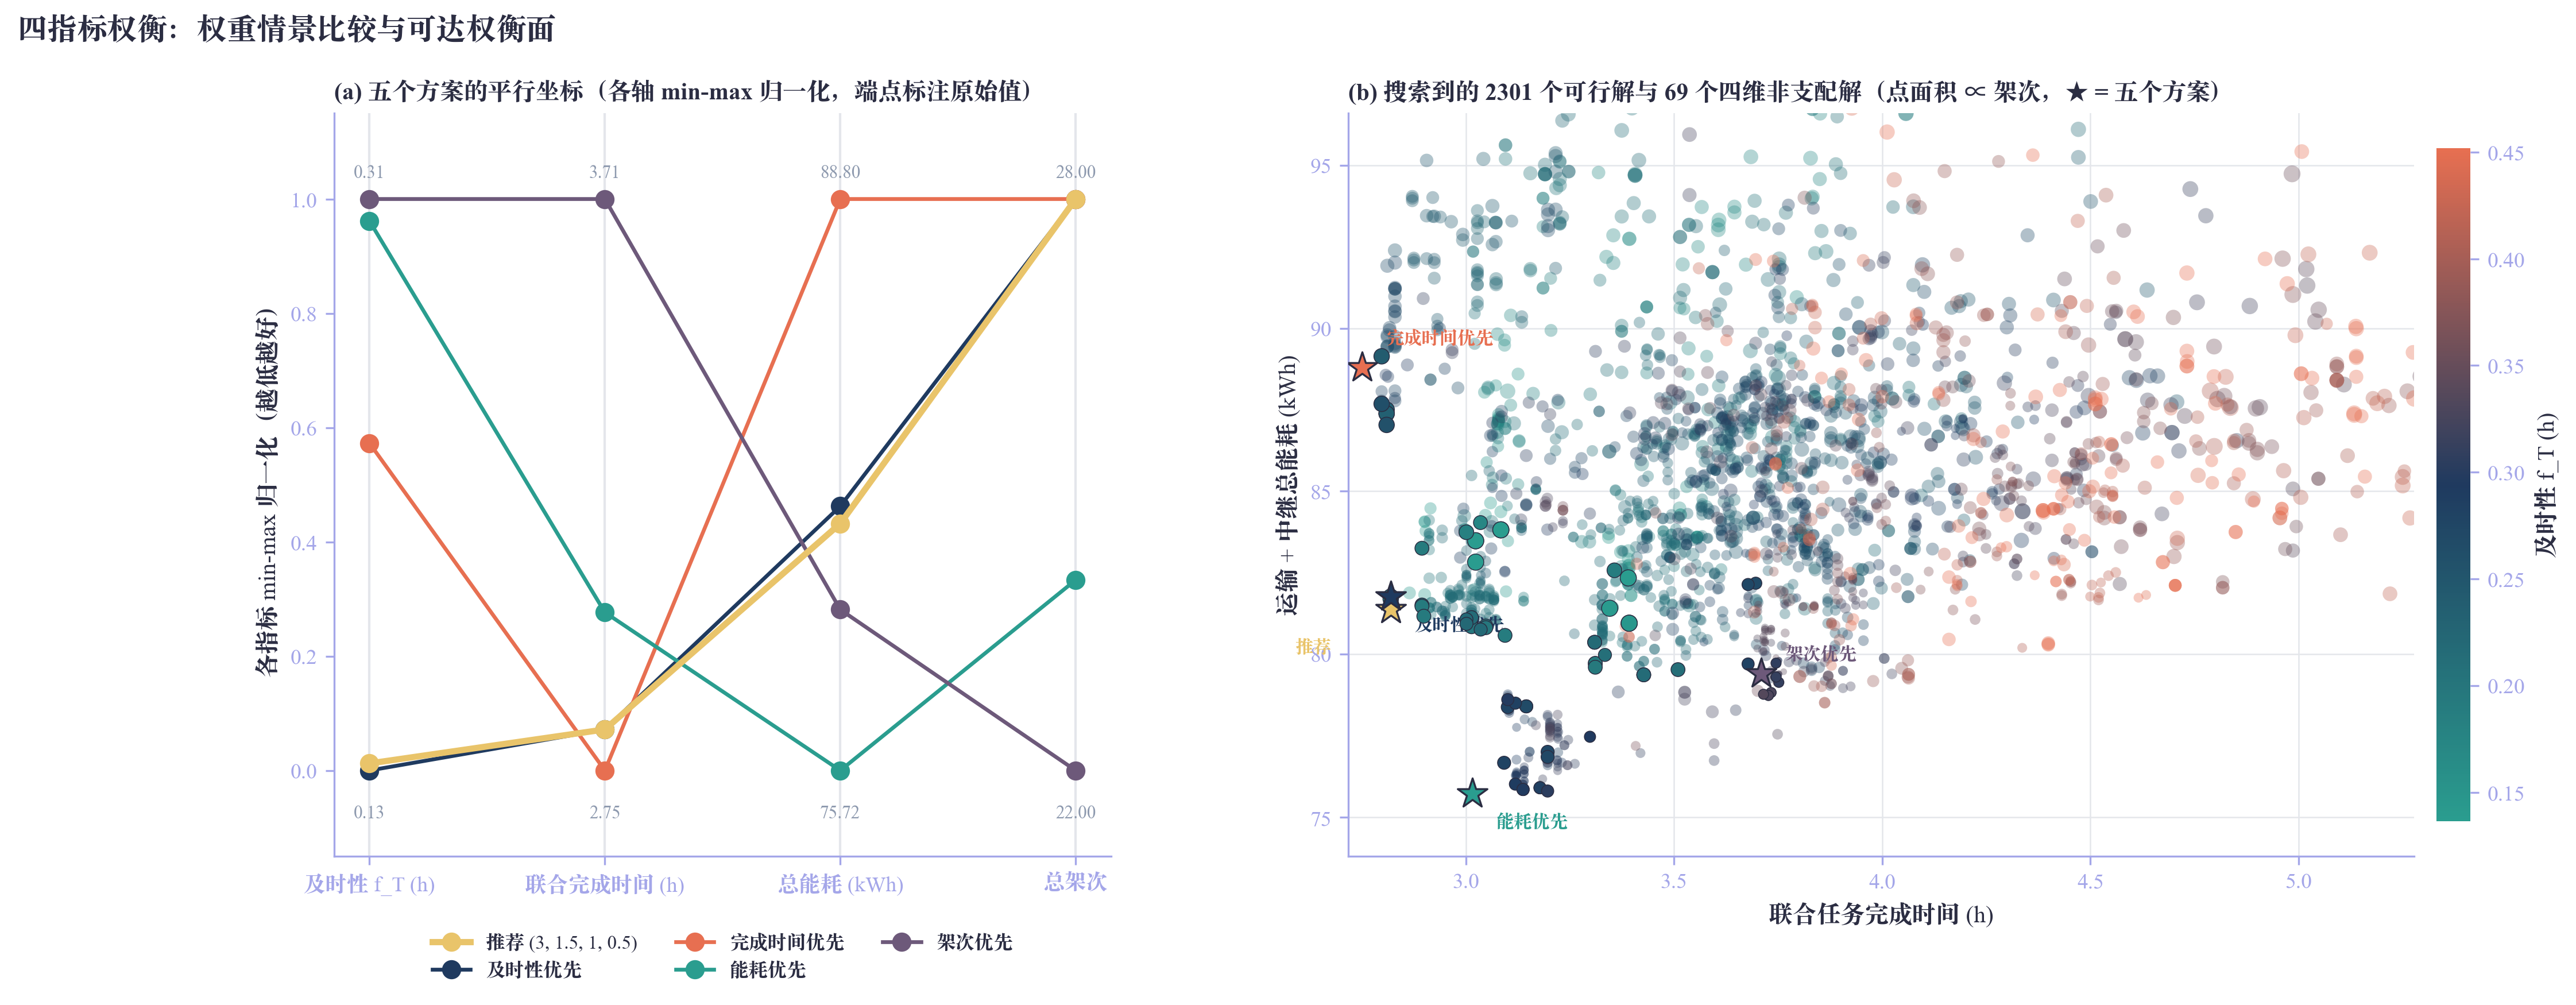
\includegraphics[width=\linewidth]{figures/Q3/图09_指标权衡.png}
\caption{不同偏好方案及搜索记录的四指标权衡}
\label{fig:q3-tradeoff}
\end{figure}

\begin{figure}[H]
\centering
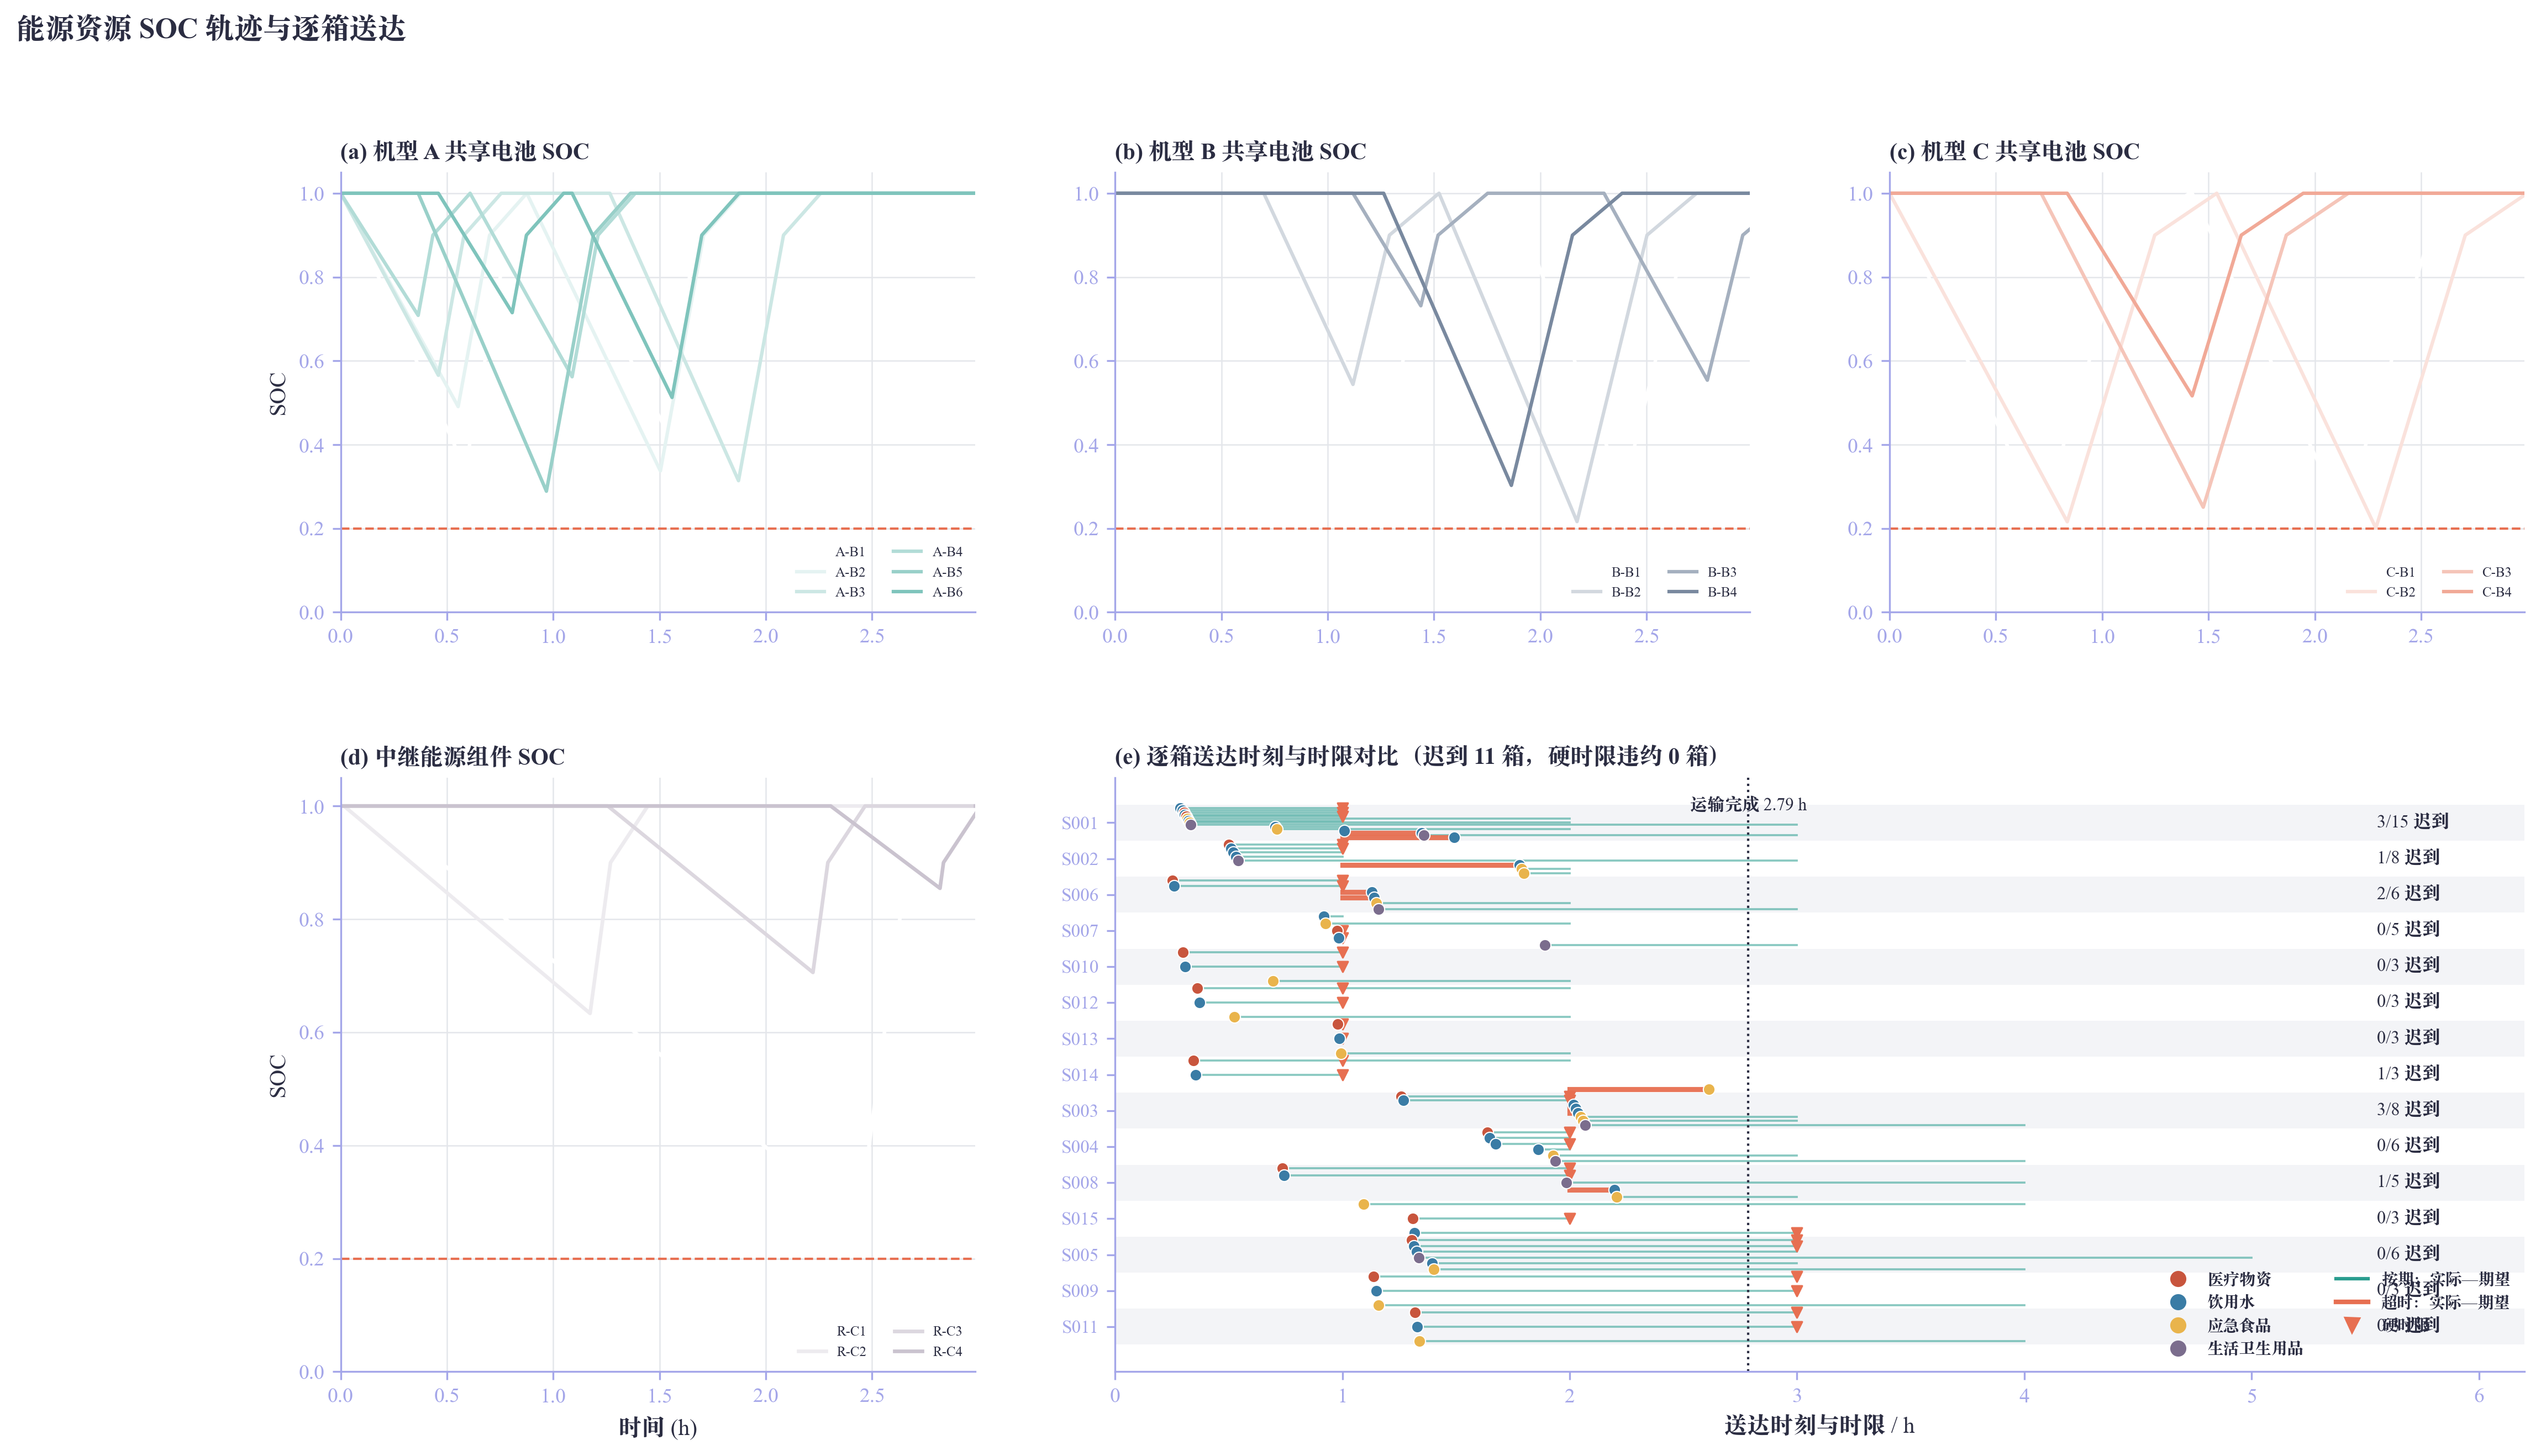
\includegraphics[width=\linewidth]{figures/Q3/图10_SOC轨迹与逐箱送达.png}
\caption{推荐联合方案的荷电状态与逐箱送达时刻}
\label{fig:q3-soc-delivery}
\end{figure}

本问的空间选址采用有限分辨率候选网格和贪心覆盖，联合排程由 ALNS 启发式求解，因而结果不构成全局最优性证明。遮挡附加损耗采用统一 $10\,\mathrm{dB}$，链路验证基于 DEM 剖面和离散轨迹采样；实际部署仍需结合天线姿态、天气衰落和现场通信测试校核。


% 第9章
\vspace{\baselineskip}
\section{问题四：救援任务分区与资源配置模型}



\subsection{问题分析}



\subsection{原子执行单元}



\subsection{固定时序下的资源需求：区间图着色}


\subsection{分区评价指标与枚举结果}


\subsection{推荐分区的资源配置方案}


\subsection{返航安全余量的敏感性分析}


\subsection{附加分析：平移架次可消解的缺口}


\subsection{本章小节}



% 第10章
\vspace{\baselineskip}
\section{模型检验与敏感性分析汇总}


\subsection{公共无力规则的一致性检验}


\subsection{方案可行性检验}




% 参考文献   手工录入
%\begin{thebibliography}{9}%宽度9
% \bibitem{bib:one} ....
% \bibitem{bib:two} ....
%\end{thebibliography}

% 采用bibtex方案
\cite{mittelbach_latex_2004,wright_latex3_2009,beeton_unicode_2008,vieth_experiences_2009}

\bibliographystyle{gmcm}
\bibliography{reference}


% 附录
\clearpage
\begin{appendices}
%\setcounter{page}{1} %如果需要可以自行重置页码。
\section{MATLAB 源程序}
\renewcommand{\thesubsection}{A\thinskip.\thinskip\arabic{subsection}}
\subsection{第1问程序}
\vspace{-2ex}

\begin{Matlab}{code.m}
clear all
kk=2;
[mdd,ndd]=size(dd);
while ~isempty(V)
    [tmpd,j]=min(W(i,V));
    tmpj=V(j);
    for k=2:ndd
        [tmp1,jj]=min(dd(1,k)+W(dd(2,k),V));
        tmp2=V(jj);
        tt(k-1,:)=[tmp1,tmp2,jj];
    end
    tmp=[tmpd,tmpj,j;tt];
    [tmp3,tmp4]=min(tmp(:,1));
    if tmp3==tmpd,
        ss(1:2,kk)=[i;tmp(tmp4,2)];
    else
        tmp5=find(ss(:,tmp4)~=0);
        tmp6=length(tmp5);
        if dd(2,tmp4)==ss(tmp6,tmp4)
            ss(1:tmp6+1,kk)=[ss(tmp5,tmp4);tmp(tmp4,2)];
        else, ss(1:3,kk)=[i;dd(2,tmp4);tmp(tmp4,2)];
        end
    end
    dd=[dd,[tmp3;tmp(tmp4,2)]];
    V(tmp(tmp4,3))=[];
    [mdd,ndd]=size(dd);kk=kk+1;
end;
S=ss; D=dd(1,:);
\end{Matlab}
\vspace{2ex}

\clearpage
\section{Python 源程序}
\renewcommand{\thesubsection}{B\thinskip.\thinskip\arabic{subsection}}
\subsection{第2问程序}
\vspace{-2ex}
\begin{Python}{mip1.py}
# This example formulates and solves the following simple MIP model:
#  maximize
#        x +   y + 2 z
#  subject to
#        x + 2 y + 3 z <= 4
#        x +   y       >= 1
#        x, y, z binary

# import gurobipy as gp
from gurobipy import * #GRB
try:
    # Create a new model
    m = Model("mip1")
    # Create variables
    x = m.addVar(vtype=GRB.BINARY, name="x")
    y = m.addVar(vtype=GRB.BINARY, name="y")
    z = m.addVar(vtype=GRB.BINARY, name="z")
    # Set objective
    m.setObjective(x + y + 2 * z, GRB.MAXIMIZE)
    # Add constraint: x + 2 y + 3 z <= 4
    m.addConstr(x + 2 * y + 3 * z <= 4, "c0")
    # Add constraint: x + y >= 1
    m.addConstr(x + y >= 1, "c1")
    # Optimize model
    m.optimize()
    for v in m.getVars():
        print('%s %g' % (v.varName, v.x))
    print('Obj: %g' % m.objVal)

except GurobiError as e:
    print('Error code ' + str(e.errno) + ': ' + str(e))

except AttributeError:
    print('Encountered an attribute error')
\end{Python}

\end{appendices}



\end{document}
